\documentclass{book}
\usepackage[a4paper,top=2.5cm,bottom=2.5cm,left=2.5cm,right=2.5cm]{geometry}
\usepackage{makeidx}
\usepackage{natbib}
\usepackage{graphicx}
\usepackage{multicol}
\usepackage{float}
\usepackage{listings}
\usepackage{color}
\usepackage{ifthen}
\usepackage[table]{xcolor}
\usepackage{textcomp}
\usepackage{alltt}
\usepackage{ifpdf}
\ifpdf
\usepackage[pdftex,
            pagebackref=true,
            colorlinks=true,
            linkcolor=blue,
            unicode
           ]{hyperref}
\else
\usepackage[ps2pdf,
            pagebackref=true,
            colorlinks=true,
            linkcolor=blue,
            unicode
           ]{hyperref}
\usepackage{pspicture}
\fi
\usepackage[utf8]{inputenc}
\usepackage{mathptmx}
\usepackage[scaled=.90]{helvet}
\usepackage{courier}
\usepackage{sectsty}
\usepackage{amssymb}
\usepackage[titles]{tocloft}
\usepackage{doxygen}
\lstset{language=C++,inputencoding=utf8,basicstyle=\footnotesize,breaklines=true,breakatwhitespace=true,tabsize=8,numbers=left }
\makeindex
\setcounter{tocdepth}{3}
\renewcommand{\footrulewidth}{0.4pt}
\renewcommand{\familydefault}{\sfdefault}
\hfuzz=15pt
\setlength{\emergencystretch}{15pt}
\hbadness=750
\tolerance=750
\begin{document}
\hypersetup{pageanchor=false,citecolor=blue}
\begin{titlepage}
\vspace*{7cm}
\begin{center}
{\Large Freya-\/\-Game \\[1ex]\large V1.\-0 }\\
\vspace*{1cm}
{\large Generated by Doxygen 1.8.1.2}\\
\vspace*{0.5cm}
{\small Sun Aug 12 2012 13:12:56}\\
\end{center}
\end{titlepage}
\clearemptydoublepage
\pagenumbering{roman}
\tableofcontents
\clearemptydoublepage
\pagenumbering{arabic}
\hypersetup{pageanchor=true,citecolor=blue}
\chapter{Main Page}
\label{index}\hypertarget{index}{} \begin{DoxyAuthor}{Authors}
Cosmin Mihai 
\end{DoxyAuthor}
\begin{DoxyVersion}{Version}
1.\-0\par
\par
 
\end{DoxyVersion}
\begin{DoxyDate}{Date}
2012 
\end{DoxyDate}
\begin{DoxyCopyright}{Copyright}
G\-N\-U Public License.
\end{DoxyCopyright}

\begin{DoxyItemize}
\item email\-: \href{mailto:yonutix@yahoo.com}{\tt yonutix@yahoo.\-com}\par

\item website\-: \href{http://www.freya.zzl.org}{\tt Freya}
\end{DoxyItemize}

\section*{Fisierele de configurare\-:}

{\bfseries Fisierul de configurare pentru obiectele statice\-:}\par
 Proiectul trebuie sa contina in radacina un fisier \char`\"{}static\-\_\-obj.\-txt\char`\"{} cu urmatorul format\-:\par
 name=\mbox{[}nume obiect\mbox{]}\par
 filename=\mbox{[}adresa obiect in format binar(vezi formatul binar al obiectelor)\mbox{]}\par
 texture=\mbox{[}adresa imaginii care va fi folosita ca textura in format T\-G\-A 8\-B uncompressed\mbox{]}\par
 poz\-X=\mbox{[}pozitia pe axa ox\mbox{]}\par
 poz\-Y=\mbox{[}pozitia pe axa oy\mbox{]}\par
 poz\-Z=\mbox{[}pozitia pe axa oz\mbox{]}\par
 angle=\mbox{[}unghiul rotatiei\mbox{]}\par
 rot\-X=\mbox{[}componenta pe ox a vectorului rotatie\mbox{]}\par
 rot\-Y=\mbox{[}componenta pe oy a vectorului rotatie\mbox{]}\par
 rot\-Z=\mbox{[}componenta pe oz a vectorului rotatie\mbox{]}\par
 scale\-X=\mbox{[}componenta pe ox a scalarii\mbox{]}\par
 scale\-Y=\mbox{[}componenta pe oy a scalarii\mbox{]}\par
 scale\-Z=\mbox{[}componenta pe oz a scalarii\mbox{]}\par
 //scale\-X, scale\-Y, scale\-Z nu sunt folosite in verisunea 1.\-0\par
 boundingbox=\mbox{[}Adresa bounding-\/box-\/ului in format bb -\/ vezi format bb\mbox{]}\par
 {\bfseries Fisierul de configurare pentru highmap}\par
 Se numeste \char`\"{}high\-Map.\-txt\char`\"{} si contine\-:\par
 lines=\mbox{[}numarul de vertecsi de-\/a lungul unei coloane\mbox{]}\par
 columns=\mbox{[}numarul de vertecsi de-\/a lungul unei linii\mbox{]}\par
 line\-Step=\mbox{[}distanta dintre 2 vertecsi de pe linii consecutive\mbox{]}\par
 column\-Step=\mbox{[}distanta dintre 2 coloane de vertecsi consecutive\mbox{]}\par
 \section*{Formate fisiere\-:}

{\bfseries .bin}\par
 Fisier binar\-:\par
 $|$\-Numar vertecsi sizeof(int)$|$\textbackslash{} v(veretex.\-x vertex.\-y vertex.\-z) sizeof(float)$\ast$ nr vertecsi $\ast$ 3 \textbackslash{}\par
 $|$\-Numar normale sizeof(int)$|$\textbackslash{} v(normala.\-x normala.\-y normala.\-z) sizeof(float)$\ast$ nr normale $\ast$ 3 \textbackslash{}\par
 $|$\-Numar coordonate textura sizeof(int)$|$\textbackslash{} v(map.\-x map.\-y) sizeof(float)$\ast$ nr normale $\ast$ 2 \textbackslash{}\par
 $|$\-Numar fete sizeof(int)$|$\textbackslash{} numar fete $\ast$ sizeof(\-Face)\textbackslash{}\par
 {\bfseries .bb}\par
 Reprezinta un set de bounding-\/box-\/uri\par
 In versiunea 1.\-0 exista 2 tipuri de bounding-\/box-\/uri\-:\par

\begin{DoxyItemize}
\item 0 Paralelipiped care este reprezentat de 6 float-\/uri(min\-Point, max\-Point)\par

\item 1 Sfera care este reprezentata de 4 float-\/uri pozitia, raza\par

\item Pe prima linie se afla numarul de bounding-\/box-\/uri\par
 pe urmaroaterele se afla informatiile despre fiecare bounding-\/box sfera sau paralelipiped\par
 
\end{DoxyItemize}
\chapter{Namespace Index}
\section{Namespace List}
Here is a list of all namespaces with brief descriptions\-:\begin{DoxyCompactList}
\item\contentsline{section}{\hyperlink{namespace_scene_settings}{Scene\-Settings} \\*Deocamdata exista doar lumini statice }{\pageref{namespace_scene_settings}}{}
\end{DoxyCompactList}

\chapter{Class Index}
\section{Class Hierarchy}
This inheritance list is sorted roughly, but not completely, alphabetically\-:\begin{DoxyCompactList}
\item \contentsline{section}{Bone}{\pageref{class_bone}}{}
\item \contentsline{section}{Bounding\-Box}{\pageref{class_bounding_box}}{}
\begin{DoxyCompactList}
\item \contentsline{section}{A\-A\-Parallelepiped}{\pageref{class_a_a_parallelepiped}}{}
\item \contentsline{section}{Sphere}{\pageref{class_sphere}}{}
\end{DoxyCompactList}
\item \contentsline{section}{Camera}{\pageref{class_camera}}{}
\item \contentsline{section}{Clasa}{\pageref{class_clasa}}{}
\item \contentsline{section}{Client}{\pageref{class_client}}{}
\item \contentsline{section}{Face}{\pageref{struct_face}}{}
\item \contentsline{section}{High\-Map}{\pageref{class_high_map}}{}
\item \contentsline{section}{Key\-Strokes}{\pageref{class_key_strokes}}{}
\item \contentsline{section}{Main\-C\-Haracter}{\pageref{class_main_c_haracter}}{}
\item \contentsline{section}{Mechanics\-Engine}{\pageref{class_mechanics_engine}}{}
\item \contentsline{section}{Menu\-G\-U\-I}{\pageref{class_menu_g_u_i}}{}
\item \contentsline{section}{Mesh\-Animation}{\pageref{class_mesh_animation}}{}
\begin{DoxyCompactList}
\item \contentsline{section}{Main\-Character}{\pageref{class_main_character}}{}
\end{DoxyCompactList}
\item \contentsline{section}{Move}{\pageref{struct_move}}{}
\item \contentsline{section}{Movie\-Intro}{\pageref{class_movie_intro}}{}
\item \contentsline{section}{object}{\pageref{structobject}}{}
\item \contentsline{section}{Point2\-D}{\pageref{struct_point2_d}}{}
\item \contentsline{section}{Static\-Obj}{\pageref{class_static_obj}}{}
\item \contentsline{section}{Targa\-Header}{\pageref{struct_targa_header}}{}
\item \contentsline{section}{Texel\-R\-G\-B}{\pageref{struct_texel_r_g_b}}{}
\item \contentsline{section}{Texel\-R\-G\-B\-A}{\pageref{struct_texel_r_g_b_a}}{}
\item \contentsline{section}{T\-G\-A\-Image}{\pageref{class_t_g_a_image}}{}
\item \contentsline{section}{Vector3}{\pageref{struct_vector3}}{}
\item \contentsline{section}{Vector3\-Int}{\pageref{struct_vector3_int}}{}
\end{DoxyCompactList}

\chapter{Class Index}
\section{Class List}
Here are the classes, structs, unions and interfaces with brief descriptions\-:\begin{DoxyCompactList}
\item\contentsline{section}{\hyperlink{class_a_a_parallelepiped}{A\-A\-Parallelepiped} }{\pageref{class_a_a_parallelepiped}}{}
\item\contentsline{section}{\hyperlink{class_bone}{Bone} }{\pageref{class_bone}}{}
\item\contentsline{section}{\hyperlink{class_bounding_box}{Bounding\-Box} }{\pageref{class_bounding_box}}{}
\item\contentsline{section}{\hyperlink{class_camera}{Camera} }{\pageref{class_camera}}{}
\item\contentsline{section}{\hyperlink{class_clasa}{Clasa} }{\pageref{class_clasa}}{}
\item\contentsline{section}{\hyperlink{class_client}{Client} }{\pageref{class_client}}{}
\item\contentsline{section}{\hyperlink{struct_face}{Face} }{\pageref{struct_face}}{}
\item\contentsline{section}{\hyperlink{class_high_map}{High\-Map} }{\pageref{class_high_map}}{}
\item\contentsline{section}{\hyperlink{class_key_strokes}{Key\-Strokes} }{\pageref{class_key_strokes}}{}
\item\contentsline{section}{\hyperlink{class_main_character}{Main\-Character} }{\pageref{class_main_character}}{}
\item\contentsline{section}{\hyperlink{class_main_c_haracter}{Main\-C\-Haracter} }{\pageref{class_main_c_haracter}}{}
\item\contentsline{section}{\hyperlink{class_mechanics_engine}{Mechanics\-Engine} }{\pageref{class_mechanics_engine}}{}
\item\contentsline{section}{\hyperlink{class_menu_g_u_i}{Menu\-G\-U\-I} }{\pageref{class_menu_g_u_i}}{}
\item\contentsline{section}{\hyperlink{class_mesh_animation}{Mesh\-Animation} }{\pageref{class_mesh_animation}}{}
\item\contentsline{section}{\hyperlink{struct_move}{Move} }{\pageref{struct_move}}{}
\item\contentsline{section}{\hyperlink{class_movie_intro}{Movie\-Intro} }{\pageref{class_movie_intro}}{}
\item\contentsline{section}{\hyperlink{structobject}{object} }{\pageref{structobject}}{}
\item\contentsline{section}{\hyperlink{struct_point2_d}{Point2\-D} }{\pageref{struct_point2_d}}{}
\item\contentsline{section}{\hyperlink{class_sphere}{Sphere} }{\pageref{class_sphere}}{}
\item\contentsline{section}{\hyperlink{class_static_obj}{Static\-Obj} }{\pageref{class_static_obj}}{}
\item\contentsline{section}{\hyperlink{struct_targa_header}{Targa\-Header} }{\pageref{struct_targa_header}}{}
\item\contentsline{section}{\hyperlink{struct_texel_r_g_b}{Texel\-R\-G\-B} }{\pageref{struct_texel_r_g_b}}{}
\item\contentsline{section}{\hyperlink{struct_texel_r_g_b_a}{Texel\-R\-G\-B\-A} }{\pageref{struct_texel_r_g_b_a}}{}
\item\contentsline{section}{\hyperlink{class_t_g_a_image}{T\-G\-A\-Image} }{\pageref{class_t_g_a_image}}{}
\item\contentsline{section}{\hyperlink{struct_vector3}{Vector3} }{\pageref{struct_vector3}}{}
\item\contentsline{section}{\hyperlink{struct_vector3_int}{Vector3\-Int} }{\pageref{struct_vector3_int}}{}
\end{DoxyCompactList}

\chapter{File Index}
\section{File List}
Here is a list of all files with brief descriptions\-:\begin{DoxyCompactList}
\item\contentsline{section}{\hyperlink{camera_8cpp}{camera.\-cpp} }{\pageref{camera_8cpp}}{}
\item\contentsline{section}{\hyperlink{camera_8h}{camera.\-h} }{\pageref{camera_8h}}{}
\item\contentsline{section}{\hyperlink{character_8cpp}{character.\-cpp} }{\pageref{character_8cpp}}{}
\item\contentsline{section}{\hyperlink{character_8h}{character.\-h} }{\pageref{character_8h}}{}
\item\contentsline{section}{\hyperlink{_client_8cpp}{Client.\-cpp} }{\pageref{_client_8cpp}}{}
\item\contentsline{section}{\hyperlink{_client_8h}{Client.\-h} }{\pageref{_client_8h}}{}
\item\contentsline{section}{\hyperlink{_comp_core_8cpp}{Comp\-Core.\-cpp} }{\pageref{_comp_core_8cpp}}{}
\item\contentsline{section}{\hyperlink{_comp_core_8h}{Comp\-Core.\-h} }{\pageref{_comp_core_8h}}{}
\item\contentsline{section}{\hyperlink{debug_8h}{debug.\-h} }{\pageref{debug_8h}}{}
\item\contentsline{section}{\hyperlink{_high_map_8cpp}{High\-Map.\-cpp} }{\pageref{_high_map_8cpp}}{}
\item\contentsline{section}{\hyperlink{_high_map_8h}{High\-Map.\-h} }{\pageref{_high_map_8h}}{}
\item\contentsline{section}{\hyperlink{key_strokes_8cpp}{key\-Strokes.\-cpp} }{\pageref{key_strokes_8cpp}}{}
\item\contentsline{section}{\hyperlink{key_strokes_8h}{key\-Strokes.\-h} }{\pageref{key_strokes_8h}}{}
\item\contentsline{section}{\hyperlink{lights_8cpp}{lights.\-cpp} }{\pageref{lights_8cpp}}{}
\item\contentsline{section}{\hyperlink{lights_8h}{lights.\-h} }{\pageref{lights_8h}}{}
\item\contentsline{section}{\hyperlink{main_8cpp}{main.\-cpp} }{\pageref{main_8cpp}}{}
\item\contentsline{section}{\hyperlink{_menu_g_u_i_8cpp}{Menu\-G\-U\-I.\-cpp} }{\pageref{_menu_g_u_i_8cpp}}{}
\item\contentsline{section}{\hyperlink{_menu_g_u_i_8h}{Menu\-G\-U\-I.\-h} }{\pageref{_menu_g_u_i_8h}}{}
\item\contentsline{section}{\hyperlink{physic_engine_8cpp}{physic\-Engine.\-cpp} }{\pageref{physic_engine_8cpp}}{}
\item\contentsline{section}{\hyperlink{physic_engine_8h}{physic\-Engine.\-h} }{\pageref{physic_engine_8h}}{}
\item\contentsline{section}{\hyperlink{sock__util_8h}{sock\-\_\-util.\-h} }{\pageref{sock__util_8h}}{}
\item\contentsline{section}{\hyperlink{static_obj_8cpp}{static\-Obj.\-cpp} }{\pageref{static_obj_8cpp}}{}
\item\contentsline{section}{\hyperlink{static_obj_8h}{static\-Obj.\-h} }{\pageref{static_obj_8h}}{}
\item\contentsline{section}{\hyperlink{_t_g_a_image_8cpp}{T\-G\-A\-Image.\-cpp} }{\pageref{_t_g_a_image_8cpp}}{}
\item\contentsline{section}{\hyperlink{_t_g_a_image_8h}{T\-G\-A\-Image.\-h} }{\pageref{_t_g_a_image_8h}}{}
\end{DoxyCompactList}

\chapter{Namespace Documentation}
\hypertarget{namespace_scene_settings}{\section{Scene\-Settings Namespace Reference}
\label{namespace_scene_settings}\index{Scene\-Settings@{Scene\-Settings}}
}


Deocamdata exista doar lumini statice.  


\subsection*{Functions}
\begin{DoxyCompactItemize}
\item 
void \hyperlink{namespace_scene_settings_a2fb1abe12509e3a90861683305984232}{initlights} ()
\begin{DoxyCompactList}\small\item\em Initializeaza luminile. \end{DoxyCompactList}\end{DoxyCompactItemize}


\subsection{Detailed Description}
Deocamdata exista doar lumini statice. 
\begin{DoxyItemize}
\item stabileste luminile 
\end{DoxyItemize}

\subsection{Function Documentation}
\hypertarget{namespace_scene_settings_a2fb1abe12509e3a90861683305984232}{\index{Scene\-Settings@{Scene\-Settings}!initlights@{initlights}}
\index{initlights@{initlights}!SceneSettings@{Scene\-Settings}}
\subsubsection[{initlights}]{\setlength{\rightskip}{0pt plus 5cm}void Scene\-Settings\-::initlights (
\begin{DoxyParamCaption}
{}
\end{DoxyParamCaption}
)}}\label{namespace_scene_settings_a2fb1abe12509e3a90861683305984232}


Initializeaza luminile. 



Definition at line 3 of file lights.\-cpp.


\chapter{Class Documentation}
\hypertarget{class_a_a_parallelepiped}{\section{A\-A\-Parallelepiped Class Reference}
\label{class_a_a_parallelepiped}\index{A\-A\-Parallelepiped@{A\-A\-Parallelepiped}}
}


{\ttfamily \#include $<$Comp\-Core.\-h$>$}

Inheritance diagram for A\-A\-Parallelepiped\-:\begin{figure}[H]
\begin{center}
\leavevmode
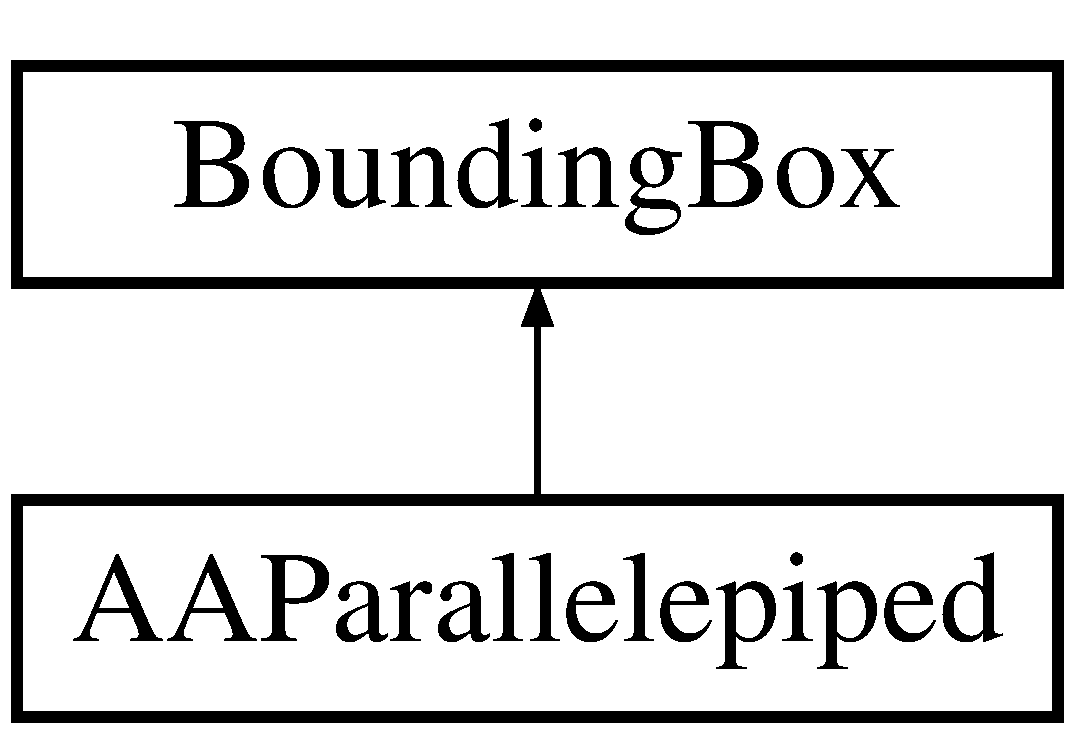
\includegraphics[height=2.000000cm]{class_a_a_parallelepiped}
\end{center}
\end{figure}
\subsection*{Public Member Functions}
\begin{DoxyCompactItemize}
\item 
\hyperlink{class_a_a_parallelepiped_acd94b7f295af0d27f89032cd44e0cead}{A\-A\-Parallelepiped} ()
\item 
\hyperlink{class_a_a_parallelepiped_a52a78b0a5253323ea67f2f3eeede75fd}{A\-A\-Parallelepiped} (\hyperlink{struct_vector3}{Vector3} \&\hyperlink{class_a_a_parallelepiped_af680a306612b1cface1885029415dd59}{min\-Point}, \hyperlink{struct_vector3}{Vector3} \&\hyperlink{class_a_a_parallelepiped_a1561fbb24fad0ebc146eec538760f863}{max\-Point})
\item 
\hyperlink{class_a_a_parallelepiped_ab6b717472bfcc5b61d6372850462865b}{A\-A\-Parallelepiped} (float min\-Pointx, float min\-Pointy, float min\-Pointz, float max\-Pointx, float max\-Pointy, float max\-Pointz)
\item 
\hyperlink{class_a_a_parallelepiped_aae402ef71b4e3b5564f5eeadd8b11365}{$\sim$\-A\-A\-Parallelepiped} ()
\item 
virtual bool \hyperlink{class_a_a_parallelepiped_ae553775bfdd16bb088710d5452aed4b4}{colide} (\hyperlink{class_bounding_box}{Bounding\-Box} $\ast$b)
\end{DoxyCompactItemize}
\subsection*{Public Attributes}
\begin{DoxyCompactItemize}
\item 
\hyperlink{struct_vector3}{Vector3} \hyperlink{class_a_a_parallelepiped_af680a306612b1cface1885029415dd59}{min\-Point}
\item 
\hyperlink{struct_vector3}{Vector3} \hyperlink{class_a_a_parallelepiped_a1561fbb24fad0ebc146eec538760f863}{max\-Point}
\end{DoxyCompactItemize}
\subsection*{Additional Inherited Members}


\subsection{Detailed Description}
Bounding box de tip paralelipiped 

Definition at line 206 of file Comp\-Core.\-h.



\subsection{Constructor \& Destructor Documentation}
\hypertarget{class_a_a_parallelepiped_acd94b7f295af0d27f89032cd44e0cead}{\index{A\-A\-Parallelepiped@{A\-A\-Parallelepiped}!A\-A\-Parallelepiped@{A\-A\-Parallelepiped}}
\index{A\-A\-Parallelepiped@{A\-A\-Parallelepiped}!AAParallelepiped@{A\-A\-Parallelepiped}}
\subsubsection[{A\-A\-Parallelepiped}]{\setlength{\rightskip}{0pt plus 5cm}A\-A\-Parallelepiped\-::\-A\-A\-Parallelepiped (
\begin{DoxyParamCaption}
{}
\end{DoxyParamCaption}
)}}\label{class_a_a_parallelepiped_acd94b7f295af0d27f89032cd44e0cead}


Definition at line 196 of file Comp\-Core.\-cpp.

\hypertarget{class_a_a_parallelepiped_a52a78b0a5253323ea67f2f3eeede75fd}{\index{A\-A\-Parallelepiped@{A\-A\-Parallelepiped}!A\-A\-Parallelepiped@{A\-A\-Parallelepiped}}
\index{A\-A\-Parallelepiped@{A\-A\-Parallelepiped}!AAParallelepiped@{A\-A\-Parallelepiped}}
\subsubsection[{A\-A\-Parallelepiped}]{\setlength{\rightskip}{0pt plus 5cm}A\-A\-Parallelepiped\-::\-A\-A\-Parallelepiped (
\begin{DoxyParamCaption}
\item[{{\bf Vector3} \&}]{min\-Point, }
\item[{{\bf Vector3} \&}]{max\-Point}
\end{DoxyParamCaption}
)}}\label{class_a_a_parallelepiped_a52a78b0a5253323ea67f2f3eeede75fd}


Definition at line 203 of file Comp\-Core.\-cpp.

\hypertarget{class_a_a_parallelepiped_ab6b717472bfcc5b61d6372850462865b}{\index{A\-A\-Parallelepiped@{A\-A\-Parallelepiped}!A\-A\-Parallelepiped@{A\-A\-Parallelepiped}}
\index{A\-A\-Parallelepiped@{A\-A\-Parallelepiped}!AAParallelepiped@{A\-A\-Parallelepiped}}
\subsubsection[{A\-A\-Parallelepiped}]{\setlength{\rightskip}{0pt plus 5cm}A\-A\-Parallelepiped\-::\-A\-A\-Parallelepiped (
\begin{DoxyParamCaption}
\item[{float}]{min\-Pointx, }
\item[{float}]{min\-Pointy, }
\item[{float}]{min\-Pointz, }
\item[{float}]{max\-Pointx, }
\item[{float}]{max\-Pointy, }
\item[{float}]{max\-Pointz}
\end{DoxyParamCaption}
)}}\label{class_a_a_parallelepiped_ab6b717472bfcc5b61d6372850462865b}


Definition at line 209 of file Comp\-Core.\-cpp.

\hypertarget{class_a_a_parallelepiped_aae402ef71b4e3b5564f5eeadd8b11365}{\index{A\-A\-Parallelepiped@{A\-A\-Parallelepiped}!$\sim$\-A\-A\-Parallelepiped@{$\sim$\-A\-A\-Parallelepiped}}
\index{$\sim$\-A\-A\-Parallelepiped@{$\sim$\-A\-A\-Parallelepiped}!AAParallelepiped@{A\-A\-Parallelepiped}}
\subsubsection[{$\sim$\-A\-A\-Parallelepiped}]{\setlength{\rightskip}{0pt plus 5cm}A\-A\-Parallelepiped\-::$\sim$\-A\-A\-Parallelepiped (
\begin{DoxyParamCaption}
{}
\end{DoxyParamCaption}
)}}\label{class_a_a_parallelepiped_aae402ef71b4e3b5564f5eeadd8b11365}


Definition at line 223 of file Comp\-Core.\-cpp.



\subsection{Member Function Documentation}
\hypertarget{class_a_a_parallelepiped_ae553775bfdd16bb088710d5452aed4b4}{\index{A\-A\-Parallelepiped@{A\-A\-Parallelepiped}!colide@{colide}}
\index{colide@{colide}!AAParallelepiped@{A\-A\-Parallelepiped}}
\subsubsection[{colide}]{\setlength{\rightskip}{0pt plus 5cm}bool A\-A\-Parallelepiped\-::colide (
\begin{DoxyParamCaption}
\item[{{\bf Bounding\-Box} $\ast$}]{b}
\end{DoxyParamCaption}
)\hspace{0.3cm}{\ttfamily [virtual]}}}\label{class_a_a_parallelepiped_ae553775bfdd16bb088710d5452aed4b4}
\begin{DoxyReturn}{Returns}
Returneaza true daca obiectul curent se ciocneste cu bounding-\/ box-\/ul 
\end{DoxyReturn}

\begin{DoxyParams}{Parameters}
{\em b} & \\
\hline
\end{DoxyParams}


Reimplemented from \hyperlink{class_bounding_box_a071b4a72196249817f7678e596011f71}{Bounding\-Box}.



Definition at line 227 of file Comp\-Core.\-cpp.



\subsection{Member Data Documentation}
\hypertarget{class_a_a_parallelepiped_a1561fbb24fad0ebc146eec538760f863}{\index{A\-A\-Parallelepiped@{A\-A\-Parallelepiped}!max\-Point@{max\-Point}}
\index{max\-Point@{max\-Point}!AAParallelepiped@{A\-A\-Parallelepiped}}
\subsubsection[{max\-Point}]{\setlength{\rightskip}{0pt plus 5cm}{\bf Vector3} A\-A\-Parallelepiped\-::max\-Point}}\label{class_a_a_parallelepiped_a1561fbb24fad0ebc146eec538760f863}


Definition at line 211 of file Comp\-Core.\-h.

\hypertarget{class_a_a_parallelepiped_af680a306612b1cface1885029415dd59}{\index{A\-A\-Parallelepiped@{A\-A\-Parallelepiped}!min\-Point@{min\-Point}}
\index{min\-Point@{min\-Point}!AAParallelepiped@{A\-A\-Parallelepiped}}
\subsubsection[{min\-Point}]{\setlength{\rightskip}{0pt plus 5cm}{\bf Vector3} A\-A\-Parallelepiped\-::min\-Point}}\label{class_a_a_parallelepiped_af680a306612b1cface1885029415dd59}

\begin{DoxyParams}{Parameters}
{\em min\-Point} & si \\
\hline
{\em max\-Point} & definesc un paralelipiped \\
\hline
\end{DoxyParams}


Definition at line 211 of file Comp\-Core.\-h.



The documentation for this class was generated from the following files\-:\begin{DoxyCompactItemize}
\item 
\hyperlink{_comp_core_8h}{Comp\-Core.\-h}\item 
\hyperlink{_comp_core_8cpp}{Comp\-Core.\-cpp}\end{DoxyCompactItemize}

\hypertarget{class_bone}{\section{Bone Class Reference}
\label{class_bone}\index{Bone@{Bone}}
}


{\ttfamily \#include $<$character.\-h$>$}

\subsection*{Public Member Functions}
\begin{DoxyCompactItemize}
\item 
\hyperlink{class_bone_ab0eb429b660fca66be1f97e6cc8de196}{Bone} ()
\item 
\hyperlink{class_bone_a8a85b84508716d1214f7fb69982d917c}{$\sim$\-Bone} ()
\end{DoxyCompactItemize}
\subsection*{Public Attributes}
\begin{DoxyCompactItemize}
\item 
\hyperlink{structobject}{object} \hyperlink{class_bone_a8e2c06c41d28182e494317a9e027f273}{section}
\item 
int \hyperlink{class_bone_abfa4a8f98163370729030745a7f1a6fb}{middle}
\item 
int \hyperlink{class_bone_a49dad9d0358f3a7aba5228243d8c9165}{in}
\item 
int \hyperlink{class_bone_a50dfae7fc1869eee97ef2eeb2602ccd7}{out}
\item 
\hyperlink{struct_vector3}{Vector3} \hyperlink{class_bone_aa011083ee788dc21828a12e16d41b5d9}{local\-In}
\item 
\hyperlink{struct_vector3}{Vector3} \hyperlink{class_bone_abb36ef81c46382b612813bb57eda48a7}{local\-Out}
\item 
\hyperlink{struct_vector3}{Vector3} \hyperlink{class_bone_a792fe0d50a7cd797e96e0418e342f1e8}{global\-In}
\item 
\hyperlink{struct_vector3}{Vector3} \hyperlink{class_bone_a1cf777430424819b626e9b2ae279ebbf}{global\-Out}
\item 
\hyperlink{class_bone}{Bone} $\ast$$\ast$ \hyperlink{class_bone_a15768d6a7d79b8d9d03f8cce8e878de6}{childs}
\end{DoxyCompactItemize}


\subsection{Detailed Description}
T\-O\-D\-O\-: O sa reprezinte un engine pentru oase si joint-\/uri, sau mai bine zis o librarie 

Definition at line 11 of file character.\-h.



\subsection{Constructor \& Destructor Documentation}
\hypertarget{class_bone_ab0eb429b660fca66be1f97e6cc8de196}{\index{Bone@{Bone}!Bone@{Bone}}
\index{Bone@{Bone}!Bone@{Bone}}
\subsubsection[{Bone}]{\setlength{\rightskip}{0pt plus 5cm}Bone\-::\-Bone (
\begin{DoxyParamCaption}
{}
\end{DoxyParamCaption}
)}}\label{class_bone_ab0eb429b660fca66be1f97e6cc8de196}


Definition at line 3 of file character.\-cpp.

\hypertarget{class_bone_a8a85b84508716d1214f7fb69982d917c}{\index{Bone@{Bone}!$\sim$\-Bone@{$\sim$\-Bone}}
\index{$\sim$\-Bone@{$\sim$\-Bone}!Bone@{Bone}}
\subsubsection[{$\sim$\-Bone}]{\setlength{\rightskip}{0pt plus 5cm}Bone\-::$\sim$\-Bone (
\begin{DoxyParamCaption}
{}
\end{DoxyParamCaption}
)}}\label{class_bone_a8a85b84508716d1214f7fb69982d917c}


Definition at line 7 of file character.\-cpp.



\subsection{Member Data Documentation}
\hypertarget{class_bone_a15768d6a7d79b8d9d03f8cce8e878de6}{\index{Bone@{Bone}!childs@{childs}}
\index{childs@{childs}!Bone@{Bone}}
\subsubsection[{childs}]{\setlength{\rightskip}{0pt plus 5cm}{\bf Bone}$\ast$$\ast$ Bone\-::childs}}\label{class_bone_a15768d6a7d79b8d9d03f8cce8e878de6}


Definition at line 17 of file character.\-h.

\hypertarget{class_bone_a792fe0d50a7cd797e96e0418e342f1e8}{\index{Bone@{Bone}!global\-In@{global\-In}}
\index{global\-In@{global\-In}!Bone@{Bone}}
\subsubsection[{global\-In}]{\setlength{\rightskip}{0pt plus 5cm}{\bf Vector3} Bone\-::global\-In}}\label{class_bone_a792fe0d50a7cd797e96e0418e342f1e8}


Definition at line 16 of file character.\-h.

\hypertarget{class_bone_a1cf777430424819b626e9b2ae279ebbf}{\index{Bone@{Bone}!global\-Out@{global\-Out}}
\index{global\-Out@{global\-Out}!Bone@{Bone}}
\subsubsection[{global\-Out}]{\setlength{\rightskip}{0pt plus 5cm}{\bf Vector3} Bone\-::global\-Out}}\label{class_bone_a1cf777430424819b626e9b2ae279ebbf}


Definition at line 16 of file character.\-h.

\hypertarget{class_bone_a49dad9d0358f3a7aba5228243d8c9165}{\index{Bone@{Bone}!in@{in}}
\index{in@{in}!Bone@{Bone}}
\subsubsection[{in}]{\setlength{\rightskip}{0pt plus 5cm}int Bone\-::in}}\label{class_bone_a49dad9d0358f3a7aba5228243d8c9165}


Definition at line 14 of file character.\-h.

\hypertarget{class_bone_aa011083ee788dc21828a12e16d41b5d9}{\index{Bone@{Bone}!local\-In@{local\-In}}
\index{local\-In@{local\-In}!Bone@{Bone}}
\subsubsection[{local\-In}]{\setlength{\rightskip}{0pt plus 5cm}{\bf Vector3} Bone\-::local\-In}}\label{class_bone_aa011083ee788dc21828a12e16d41b5d9}


Definition at line 15 of file character.\-h.

\hypertarget{class_bone_abb36ef81c46382b612813bb57eda48a7}{\index{Bone@{Bone}!local\-Out@{local\-Out}}
\index{local\-Out@{local\-Out}!Bone@{Bone}}
\subsubsection[{local\-Out}]{\setlength{\rightskip}{0pt plus 5cm}{\bf Vector3} Bone\-::local\-Out}}\label{class_bone_abb36ef81c46382b612813bb57eda48a7}


Definition at line 15 of file character.\-h.

\hypertarget{class_bone_abfa4a8f98163370729030745a7f1a6fb}{\index{Bone@{Bone}!middle@{middle}}
\index{middle@{middle}!Bone@{Bone}}
\subsubsection[{middle}]{\setlength{\rightskip}{0pt plus 5cm}int Bone\-::middle}}\label{class_bone_abfa4a8f98163370729030745a7f1a6fb}


Definition at line 14 of file character.\-h.

\hypertarget{class_bone_a50dfae7fc1869eee97ef2eeb2602ccd7}{\index{Bone@{Bone}!out@{out}}
\index{out@{out}!Bone@{Bone}}
\subsubsection[{out}]{\setlength{\rightskip}{0pt plus 5cm}int Bone\-::out}}\label{class_bone_a50dfae7fc1869eee97ef2eeb2602ccd7}


Definition at line 14 of file character.\-h.

\hypertarget{class_bone_a8e2c06c41d28182e494317a9e027f273}{\index{Bone@{Bone}!section@{section}}
\index{section@{section}!Bone@{Bone}}
\subsubsection[{section}]{\setlength{\rightskip}{0pt plus 5cm}{\bf object} Bone\-::section}}\label{class_bone_a8e2c06c41d28182e494317a9e027f273}


Definition at line 13 of file character.\-h.



The documentation for this class was generated from the following files\-:\begin{DoxyCompactItemize}
\item 
\hyperlink{character_8h}{character.\-h}\item 
\hyperlink{character_8cpp}{character.\-cpp}\end{DoxyCompactItemize}

\hypertarget{class_bounding_box}{\section{Bounding\-Box Class Reference}
\label{class_bounding_box}\index{Bounding\-Box@{Bounding\-Box}}
}


{\ttfamily \#include $<$Comp\-Core.\-h$>$}

Inheritance diagram for Bounding\-Box\-:\begin{figure}[H]
\begin{center}
\leavevmode
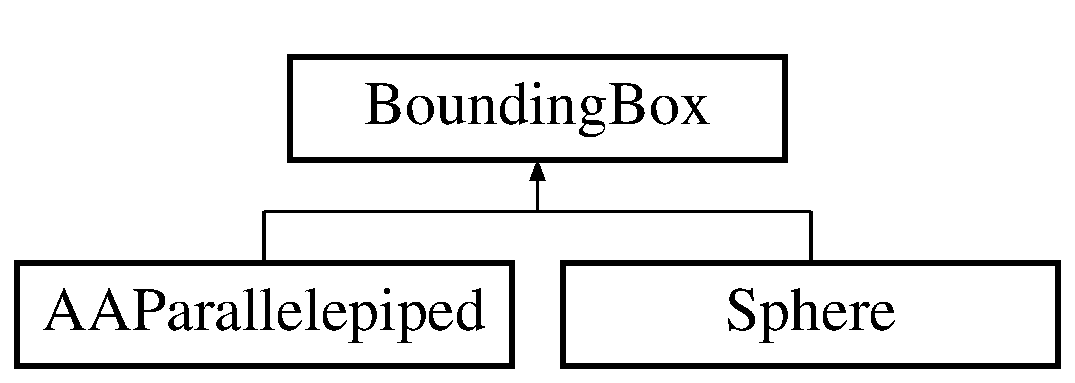
\includegraphics[height=2.000000cm]{class_bounding_box}
\end{center}
\end{figure}
\subsection*{Public Types}
\begin{DoxyCompactItemize}
\item 
enum \{ \hyperlink{class_bounding_box_ac4eb5027a54b684f95999bea905ce3e1a8d808e5d8708319c327450ed8cf4c335}{S\-P\-H\-E\-R\-E}, 
\hyperlink{class_bounding_box_ac4eb5027a54b684f95999bea905ce3e1ada5242406c5801cdb1d436b277503853}{P\-A\-R\-A\-L\-L\-E\-L\-E\-P\-I\-P\-E\-D}
 \}
\begin{DoxyCompactList}\small\item\em Se poate dezvolta aplicatia astfel incat un bounding-\/box sa fie de oricate forme. \end{DoxyCompactList}\end{DoxyCompactItemize}
\subsection*{Public Member Functions}
\begin{DoxyCompactItemize}
\item 
\hyperlink{class_bounding_box_a6e401c4da5839950f1f30c8b8c4d1208}{Bounding\-Box} ()
\item 
\hyperlink{class_bounding_box_a587de78331711c6eb6d15de867b73991}{$\sim$\-Bounding\-Box} ()
\item 
virtual bool \hyperlink{class_bounding_box_a071b4a72196249817f7678e596011f71}{colide} (\hyperlink{class_bounding_box}{Bounding\-Box} $\ast$b)
\item 
int \hyperlink{class_bounding_box_ae55e5dec2bfab0f338851af88e4980e5}{get\-Type} () const 
\end{DoxyCompactItemize}
\subsection*{Public Attributes}
\begin{DoxyCompactItemize}
\item 
int \hyperlink{class_bounding_box_a87e612000c8e4af69aa7c3060ff6e77d}{type}
\end{DoxyCompactItemize}


\subsection{Detailed Description}
pentru bounding-\/box-\/uri 

Definition at line 181 of file Comp\-Core.\-h.



\subsection{Member Enumeration Documentation}
\hypertarget{class_bounding_box_ac4eb5027a54b684f95999bea905ce3e1}{\subsubsection[{anonymous enum}]{\setlength{\rightskip}{0pt plus 5cm}anonymous enum}}\label{class_bounding_box_ac4eb5027a54b684f95999bea905ce3e1}


Se poate dezvolta aplicatia astfel incat un bounding-\/box sa fie de oricate forme. 

\begin{Desc}
\item[Enumerator\-: ]\par
\begin{description}
\index{S\-P\-H\-E\-R\-E@{S\-P\-H\-E\-R\-E}!Bounding\-Box@{Bounding\-Box}}\index{Bounding\-Box@{Bounding\-Box}!S\-P\-H\-E\-R\-E@{S\-P\-H\-E\-R\-E}}\item[{\em 
\hypertarget{class_bounding_box_ac4eb5027a54b684f95999bea905ce3e1a8d808e5d8708319c327450ed8cf4c335}{S\-P\-H\-E\-R\-E}\label{class_bounding_box_ac4eb5027a54b684f95999bea905ce3e1a8d808e5d8708319c327450ed8cf4c335}
}]\index{P\-A\-R\-A\-L\-L\-E\-L\-E\-P\-I\-P\-E\-D@{P\-A\-R\-A\-L\-L\-E\-L\-E\-P\-I\-P\-E\-D}!Bounding\-Box@{Bounding\-Box}}\index{Bounding\-Box@{Bounding\-Box}!P\-A\-R\-A\-L\-L\-E\-L\-E\-P\-I\-P\-E\-D@{P\-A\-R\-A\-L\-L\-E\-L\-E\-P\-I\-P\-E\-D}}\item[{\em 
\hypertarget{class_bounding_box_ac4eb5027a54b684f95999bea905ce3e1ada5242406c5801cdb1d436b277503853}{P\-A\-R\-A\-L\-L\-E\-L\-E\-P\-I\-P\-E\-D}\label{class_bounding_box_ac4eb5027a54b684f95999bea905ce3e1ada5242406c5801cdb1d436b277503853}
}]\end{description}
\end{Desc}



Definition at line 187 of file Comp\-Core.\-h.



\subsection{Constructor \& Destructor Documentation}
\hypertarget{class_bounding_box_a6e401c4da5839950f1f30c8b8c4d1208}{\index{Bounding\-Box@{Bounding\-Box}!Bounding\-Box@{Bounding\-Box}}
\index{Bounding\-Box@{Bounding\-Box}!BoundingBox@{Bounding\-Box}}
\subsubsection[{Bounding\-Box}]{\setlength{\rightskip}{0pt plus 5cm}Bounding\-Box\-::\-Bounding\-Box (
\begin{DoxyParamCaption}
{}
\end{DoxyParamCaption}
)}}\label{class_bounding_box_a6e401c4da5839950f1f30c8b8c4d1208}


Definition at line 179 of file Comp\-Core.\-cpp.

\hypertarget{class_bounding_box_a587de78331711c6eb6d15de867b73991}{\index{Bounding\-Box@{Bounding\-Box}!$\sim$\-Bounding\-Box@{$\sim$\-Bounding\-Box}}
\index{$\sim$\-Bounding\-Box@{$\sim$\-Bounding\-Box}!BoundingBox@{Bounding\-Box}}
\subsubsection[{$\sim$\-Bounding\-Box}]{\setlength{\rightskip}{0pt plus 5cm}Bounding\-Box\-::$\sim$\-Bounding\-Box (
\begin{DoxyParamCaption}
{}
\end{DoxyParamCaption}
)}}\label{class_bounding_box_a587de78331711c6eb6d15de867b73991}


Definition at line 183 of file Comp\-Core.\-cpp.



\subsection{Member Function Documentation}
\hypertarget{class_bounding_box_a071b4a72196249817f7678e596011f71}{\index{Bounding\-Box@{Bounding\-Box}!colide@{colide}}
\index{colide@{colide}!BoundingBox@{Bounding\-Box}}
\subsubsection[{colide}]{\setlength{\rightskip}{0pt plus 5cm}bool Bounding\-Box\-::colide (
\begin{DoxyParamCaption}
\item[{{\bf Bounding\-Box} $\ast$}]{b}
\end{DoxyParamCaption}
)\hspace{0.3cm}{\ttfamily [virtual]}}}\label{class_bounding_box_a071b4a72196249817f7678e596011f71}


Reimplemented in \hyperlink{class_a_a_parallelepiped_ae553775bfdd16bb088710d5452aed4b4}{A\-A\-Parallelepiped}.



Definition at line 187 of file Comp\-Core.\-cpp.

\hypertarget{class_bounding_box_ae55e5dec2bfab0f338851af88e4980e5}{\index{Bounding\-Box@{Bounding\-Box}!get\-Type@{get\-Type}}
\index{get\-Type@{get\-Type}!BoundingBox@{Bounding\-Box}}
\subsubsection[{get\-Type}]{\setlength{\rightskip}{0pt plus 5cm}int Bounding\-Box\-::get\-Type (
\begin{DoxyParamCaption}
{}
\end{DoxyParamCaption}
) const\hspace{0.3cm}{\ttfamily [inline]}}}\label{class_bounding_box_ae55e5dec2bfab0f338851af88e4980e5}
\begin{DoxyReturn}{Returns}
Returneaza tipul bounding box-\/ului 
\end{DoxyReturn}


Definition at line 200 of file Comp\-Core.\-h.



\subsection{Member Data Documentation}
\hypertarget{class_bounding_box_a87e612000c8e4af69aa7c3060ff6e77d}{\index{Bounding\-Box@{Bounding\-Box}!type@{type}}
\index{type@{type}!BoundingBox@{Bounding\-Box}}
\subsubsection[{type}]{\setlength{\rightskip}{0pt plus 5cm}int Bounding\-Box\-::type}}\label{class_bounding_box_a87e612000c8e4af69aa7c3060ff6e77d}

\begin{DoxyParams}{Parameters}
{\em tipul} & frame-\/ului este folosit pentru a cunoaste clasa derivata la care se face cast \\
\hline
\end{DoxyParams}


Definition at line 192 of file Comp\-Core.\-h.



The documentation for this class was generated from the following files\-:\begin{DoxyCompactItemize}
\item 
\hyperlink{_comp_core_8h}{Comp\-Core.\-h}\item 
\hyperlink{_comp_core_8cpp}{Comp\-Core.\-cpp}\end{DoxyCompactItemize}

\hypertarget{class_camera}{\section{Camera Class Reference}
\label{class_camera}\index{Camera@{Camera}}
}


{\ttfamily \#include $<$camera.\-h$>$}

\subsection*{Public Member Functions}
\begin{DoxyCompactItemize}
\item 
\hyperlink{class_camera_a01f94c3543f56ede7af49dc778f19331}{Camera} ()
\begin{DoxyCompactList}\small\item\em Initializarea camerei se face la pozitia (0, 0, 0) cu rotatie (0, 0, 0) si scale(1, 1, 1) \end{DoxyCompactList}\item 
\hyperlink{class_camera_ad1897942d0ccf91052386388a497349f}{$\sim$\-Camera} ()
\item 
void \hyperlink{class_camera_a73ccd8097845e13876fc693c5e614d90}{set\-Translation} (\hyperlink{struct_vector3}{Vector3} \&point)
\begin{DoxyCompactList}\small\item\em Schimba pozitia la pozitia {\bfseries new\-Point} \end{DoxyCompactList}\item 
void \hyperlink{class_camera_aba9df9fb2129b591d26bb5419318355d}{set\-Rotation} (\hyperlink{struct_vector3}{Vector3} \&new\-Axis)
\begin{DoxyCompactList}\small\item\em Schimba vectorul in jurul careia se desfasoara rotatia la vectorul new\-Axis, ar fi o idee buna sa primeasca ca parametru un quaternion. \end{DoxyCompactList}\item 
void \hyperlink{class_camera_ac6edf32fdd18fbd064255beefc9ceca2}{set\-Scale} (\hyperlink{struct_vector3}{Vector3} \&new\-Size)
\begin{DoxyCompactList}\small\item\em Seteaza scalarea la dimensiunile new\-Size  Netestata! \end{DoxyCompactList}\item 
void \hyperlink{class_camera_a8d10ea5b8790919325234395c7b04a6f}{move\-Forward} (float step)
\begin{DoxyCompactList}\small\item\em Muta camera inainte oricare ar fi orientarea acesteia. \end{DoxyCompactList}\item 
void \hyperlink{class_camera_a2a687c711d5f46a6c9de4513c4e334cc}{move\-Backward} (float step)
\begin{DoxyCompactList}\small\item\em Muta camera inapoi oricare ar fi orientarea acesteia. \end{DoxyCompactList}\item 
void \hyperlink{class_camera_a9733e299c281288208e4ce36681143a6}{move\-Left} (float step)
\begin{DoxyCompactList}\small\item\em Muta camera spre stanga oricare ar fi orientarea acesteia. \end{DoxyCompactList}\item 
void \hyperlink{class_camera_a70f638369d8bbcb60639f5b1cc40de19}{move\-Right} (float step)
\begin{DoxyCompactList}\small\item\em Muta camera spre dreapta oricare ar fi orientarea acesteia. \end{DoxyCompactList}\item 
void \hyperlink{class_camera_a61e15d0587412375261ca39de2f4776b}{rotate\-Left} (float step)
\begin{DoxyCompactList}\small\item\em Roteste camera spre stanga. \end{DoxyCompactList}\item 
void \hyperlink{class_camera_a149d10b600ac1d5b91430cdf9a3dae7d}{rotate\-Right} (float step)
\begin{DoxyCompactList}\small\item\em Roteste camera spre dreapta. \end{DoxyCompactList}\item 
void \hyperlink{class_camera_a5499e626fe539645aa4831369e93851a}{make\-Move} () const 
\begin{DoxyCompactList}\small\item\em Efectueaza mutarea dupa metoda rotate-\/translate. \end{DoxyCompactList}\item 
void \hyperlink{class_camera_aeb07ceb5fc0f41709f3fdfa13c87252c}{make\-Rotation} () const 
\begin{DoxyCompactList}\small\item\em Efecturaza rotatia in jurul axei oy. \end{DoxyCompactList}\item 
void \hyperlink{class_camera_aa2d535ba7952ee33c37e84461d57f1c2}{make\-Translation} () const 
\begin{DoxyCompactList}\small\item\em Efectueaza translatia camerei. \end{DoxyCompactList}\item 
void \hyperlink{class_camera_a02be8aa0dbef77e02dddc715a726fb67}{reset} ()
\begin{DoxyCompactList}\small\item\em Reseteaza pozitia camerei la cea initiala. \end{DoxyCompactList}\item 
virtual void \hyperlink{class_camera_a303cfefa7f5d925e911000cf3fbdfd39}{get\-Position} ()
\begin{DoxyCompactList}\small\item\em Seteaza inaltimea la care se gaseste camera conform high\-Map-\/ului Nu functioneaza foarte bine T\-O\-D\-O -\/ analizat bug-\/uri. \end{DoxyCompactList}\end{DoxyCompactItemize}
\subsection*{Public Attributes}
\begin{DoxyCompactItemize}
\item 
\hyperlink{struct_vector3}{Vector3} \hyperlink{class_camera_ad86bc5edaaf030fa76edac96040e56f4}{translation}
\item 
\hyperlink{struct_vector3}{Vector3} \hyperlink{class_camera_a49d1e42b190a89485c29b6a0bd0fb19b}{rotation}
\item 
\hyperlink{struct_vector3}{Vector3} \hyperlink{class_camera_a048f3227386a7874d82d5a955eab803c}{scale}
\item 
\hyperlink{struct_vector3}{Vector3} \hyperlink{class_camera_aa2e21e07158e70c900e1a8473b4e96d7}{undo\-\_\-translation}
\end{DoxyCompactItemize}


\subsection{Detailed Description}
class \hyperlink{class_camera}{Camera} -\/ \hyperlink{class_clasa}{Clasa} care reprezinta camera controlata de utilizator Foloseste metoda rotate-\/translate nu gl\-Look\-At, in contextul curent este discutabila schimbarea implementarii, dar este foarte probabil ca ar duce la un rezultat bun 

Definition at line 19 of file camera.\-h.



\subsection{Constructor \& Destructor Documentation}
\hypertarget{class_camera_a01f94c3543f56ede7af49dc778f19331}{\index{Camera@{Camera}!Camera@{Camera}}
\index{Camera@{Camera}!Camera@{Camera}}
\subsubsection[{Camera}]{\setlength{\rightskip}{0pt plus 5cm}Camera\-::\-Camera (
\begin{DoxyParamCaption}
{}
\end{DoxyParamCaption}
)}}\label{class_camera_a01f94c3543f56ede7af49dc778f19331}


Initializarea camerei se face la pozitia (0, 0, 0) cu rotatie (0, 0, 0) si scale(1, 1, 1) 



Definition at line 6 of file camera.\-cpp.

\hypertarget{class_camera_ad1897942d0ccf91052386388a497349f}{\index{Camera@{Camera}!$\sim$\-Camera@{$\sim$\-Camera}}
\index{$\sim$\-Camera@{$\sim$\-Camera}!Camera@{Camera}}
\subsubsection[{$\sim$\-Camera}]{\setlength{\rightskip}{0pt plus 5cm}Camera\-::$\sim$\-Camera (
\begin{DoxyParamCaption}
{}
\end{DoxyParamCaption}
)}}\label{class_camera_ad1897942d0ccf91052386388a497349f}


Definition at line 13 of file camera.\-cpp.



\subsection{Member Function Documentation}
\hypertarget{class_camera_a303cfefa7f5d925e911000cf3fbdfd39}{\index{Camera@{Camera}!get\-Position@{get\-Position}}
\index{get\-Position@{get\-Position}!Camera@{Camera}}
\subsubsection[{get\-Position}]{\setlength{\rightskip}{0pt plus 5cm}void Camera\-::get\-Position (
\begin{DoxyParamCaption}
{}
\end{DoxyParamCaption}
)\hspace{0.3cm}{\ttfamily [virtual]}}}\label{class_camera_a303cfefa7f5d925e911000cf3fbdfd39}


Seteaza inaltimea la care se gaseste camera conform high\-Map-\/ului Nu functioneaza foarte bine T\-O\-D\-O -\/ analizat bug-\/uri. 



Definition at line 95 of file camera.\-cpp.

\hypertarget{class_camera_a5499e626fe539645aa4831369e93851a}{\index{Camera@{Camera}!make\-Move@{make\-Move}}
\index{make\-Move@{make\-Move}!Camera@{Camera}}
\subsubsection[{make\-Move}]{\setlength{\rightskip}{0pt plus 5cm}void Camera\-::make\-Move (
\begin{DoxyParamCaption}
{}
\end{DoxyParamCaption}
) const\hspace{0.3cm}{\ttfamily [inline]}}}\label{class_camera_a5499e626fe539645aa4831369e93851a}


Efectueaza mutarea dupa metoda rotate-\/translate. 



Definition at line 91 of file camera.\-h.

\hypertarget{class_camera_aeb07ceb5fc0f41709f3fdfa13c87252c}{\index{Camera@{Camera}!make\-Rotation@{make\-Rotation}}
\index{make\-Rotation@{make\-Rotation}!Camera@{Camera}}
\subsubsection[{make\-Rotation}]{\setlength{\rightskip}{0pt plus 5cm}void Camera\-::make\-Rotation (
\begin{DoxyParamCaption}
{}
\end{DoxyParamCaption}
) const\hspace{0.3cm}{\ttfamily [inline]}}}\label{class_camera_aeb07ceb5fc0f41709f3fdfa13c87252c}


Efecturaza rotatia in jurul axei oy. 



Definition at line 100 of file camera.\-h.

\hypertarget{class_camera_aa2d535ba7952ee33c37e84461d57f1c2}{\index{Camera@{Camera}!make\-Translation@{make\-Translation}}
\index{make\-Translation@{make\-Translation}!Camera@{Camera}}
\subsubsection[{make\-Translation}]{\setlength{\rightskip}{0pt plus 5cm}void Camera\-::make\-Translation (
\begin{DoxyParamCaption}
{}
\end{DoxyParamCaption}
) const\hspace{0.3cm}{\ttfamily [inline]}}}\label{class_camera_aa2d535ba7952ee33c37e84461d57f1c2}


Efectueaza translatia camerei. 



Definition at line 105 of file camera.\-h.

\hypertarget{class_camera_a2a687c711d5f46a6c9de4513c4e334cc}{\index{Camera@{Camera}!move\-Backward@{move\-Backward}}
\index{move\-Backward@{move\-Backward}!Camera@{Camera}}
\subsubsection[{move\-Backward}]{\setlength{\rightskip}{0pt plus 5cm}void Camera\-::move\-Backward (
\begin{DoxyParamCaption}
\item[{float}]{step}
\end{DoxyParamCaption}
)}}\label{class_camera_a2a687c711d5f46a6c9de4513c4e334cc}


Muta camera inapoi oricare ar fi orientarea acesteia. 



Definition at line 45 of file camera.\-cpp.

\hypertarget{class_camera_a8d10ea5b8790919325234395c7b04a6f}{\index{Camera@{Camera}!move\-Forward@{move\-Forward}}
\index{move\-Forward@{move\-Forward}!Camera@{Camera}}
\subsubsection[{move\-Forward}]{\setlength{\rightskip}{0pt plus 5cm}void Camera\-::move\-Forward (
\begin{DoxyParamCaption}
\item[{float}]{step}
\end{DoxyParamCaption}
)}}\label{class_camera_a8d10ea5b8790919325234395c7b04a6f}


Muta camera inainte oricare ar fi orientarea acesteia. 


\begin{DoxyParams}{Parameters}
{\em step} & Distanta pe care se face avansarea \\
\hline
\end{DoxyParams}


Definition at line 38 of file camera.\-cpp.

\hypertarget{class_camera_a9733e299c281288208e4ce36681143a6}{\index{Camera@{Camera}!move\-Left@{move\-Left}}
\index{move\-Left@{move\-Left}!Camera@{Camera}}
\subsubsection[{move\-Left}]{\setlength{\rightskip}{0pt plus 5cm}void Camera\-::move\-Left (
\begin{DoxyParamCaption}
\item[{float}]{step}
\end{DoxyParamCaption}
)}}\label{class_camera_a9733e299c281288208e4ce36681143a6}


Muta camera spre stanga oricare ar fi orientarea acesteia. 



Definition at line 52 of file camera.\-cpp.

\hypertarget{class_camera_a70f638369d8bbcb60639f5b1cc40de19}{\index{Camera@{Camera}!move\-Right@{move\-Right}}
\index{move\-Right@{move\-Right}!Camera@{Camera}}
\subsubsection[{move\-Right}]{\setlength{\rightskip}{0pt plus 5cm}void Camera\-::move\-Right (
\begin{DoxyParamCaption}
\item[{float}]{step}
\end{DoxyParamCaption}
)}}\label{class_camera_a70f638369d8bbcb60639f5b1cc40de19}


Muta camera spre dreapta oricare ar fi orientarea acesteia. 



Definition at line 59 of file camera.\-cpp.

\hypertarget{class_camera_a02be8aa0dbef77e02dddc715a726fb67}{\index{Camera@{Camera}!reset@{reset}}
\index{reset@{reset}!Camera@{Camera}}
\subsubsection[{reset}]{\setlength{\rightskip}{0pt plus 5cm}void Camera\-::reset (
\begin{DoxyParamCaption}
{}
\end{DoxyParamCaption}
)}}\label{class_camera_a02be8aa0dbef77e02dddc715a726fb67}


Reseteaza pozitia camerei la cea initiala. 



Definition at line 88 of file camera.\-cpp.

\hypertarget{class_camera_a61e15d0587412375261ca39de2f4776b}{\index{Camera@{Camera}!rotate\-Left@{rotate\-Left}}
\index{rotate\-Left@{rotate\-Left}!Camera@{Camera}}
\subsubsection[{rotate\-Left}]{\setlength{\rightskip}{0pt plus 5cm}void Camera\-::rotate\-Left (
\begin{DoxyParamCaption}
\item[{float}]{step}
\end{DoxyParamCaption}
)}}\label{class_camera_a61e15d0587412375261ca39de2f4776b}


Roteste camera spre stanga. 



Definition at line 66 of file camera.\-cpp.

\hypertarget{class_camera_a149d10b600ac1d5b91430cdf9a3dae7d}{\index{Camera@{Camera}!rotate\-Right@{rotate\-Right}}
\index{rotate\-Right@{rotate\-Right}!Camera@{Camera}}
\subsubsection[{rotate\-Right}]{\setlength{\rightskip}{0pt plus 5cm}void Camera\-::rotate\-Right (
\begin{DoxyParamCaption}
\item[{float}]{step}
\end{DoxyParamCaption}
)}}\label{class_camera_a149d10b600ac1d5b91430cdf9a3dae7d}


Roteste camera spre dreapta. 



Definition at line 77 of file camera.\-cpp.

\hypertarget{class_camera_aba9df9fb2129b591d26bb5419318355d}{\index{Camera@{Camera}!set\-Rotation@{set\-Rotation}}
\index{set\-Rotation@{set\-Rotation}!Camera@{Camera}}
\subsubsection[{set\-Rotation}]{\setlength{\rightskip}{0pt plus 5cm}void Camera\-::set\-Rotation (
\begin{DoxyParamCaption}
\item[{{\bf Vector3} \&}]{new\-Axis}
\end{DoxyParamCaption}
)}}\label{class_camera_aba9df9fb2129b591d26bb5419318355d}


Schimba vectorul in jurul careia se desfasoara rotatia la vectorul new\-Axis, ar fi o idee buna sa primeasca ca parametru un quaternion. 



Definition at line 24 of file camera.\-cpp.

\hypertarget{class_camera_ac6edf32fdd18fbd064255beefc9ceca2}{\index{Camera@{Camera}!set\-Scale@{set\-Scale}}
\index{set\-Scale@{set\-Scale}!Camera@{Camera}}
\subsubsection[{set\-Scale}]{\setlength{\rightskip}{0pt plus 5cm}void Camera\-::set\-Scale (
\begin{DoxyParamCaption}
\item[{{\bf Vector3} \&}]{new\-Size}
\end{DoxyParamCaption}
)}}\label{class_camera_ac6edf32fdd18fbd064255beefc9ceca2}


Seteaza scalarea la dimensiunile new\-Size  Netestata! 



Definition at line 31 of file camera.\-cpp.

\hypertarget{class_camera_a73ccd8097845e13876fc693c5e614d90}{\index{Camera@{Camera}!set\-Translation@{set\-Translation}}
\index{set\-Translation@{set\-Translation}!Camera@{Camera}}
\subsubsection[{set\-Translation}]{\setlength{\rightskip}{0pt plus 5cm}void Camera\-::set\-Translation (
\begin{DoxyParamCaption}
\item[{{\bf Vector3} \&}]{point}
\end{DoxyParamCaption}
)}}\label{class_camera_a73ccd8097845e13876fc693c5e614d90}


Schimba pozitia la pozitia {\bfseries new\-Point} 


\begin{DoxyParams}{Parameters}
{\em new\-Point} & \\
\hline
\end{DoxyParams}


Definition at line 17 of file camera.\-cpp.



\subsection{Member Data Documentation}
\hypertarget{class_camera_a49d1e42b190a89485c29b6a0bd0fb19b}{\index{Camera@{Camera}!rotation@{rotation}}
\index{rotation@{rotation}!Camera@{Camera}}
\subsubsection[{rotation}]{\setlength{\rightskip}{0pt plus 5cm}{\bf Vector3} Camera\-::rotation}}\label{class_camera_a49d1e42b190a89485c29b6a0bd0fb19b}


Definition at line 21 of file camera.\-h.

\hypertarget{class_camera_a048f3227386a7874d82d5a955eab803c}{\index{Camera@{Camera}!scale@{scale}}
\index{scale@{scale}!Camera@{Camera}}
\subsubsection[{scale}]{\setlength{\rightskip}{0pt plus 5cm}{\bf Vector3} Camera\-::scale}}\label{class_camera_a048f3227386a7874d82d5a955eab803c}


Definition at line 21 of file camera.\-h.

\hypertarget{class_camera_ad86bc5edaaf030fa76edac96040e56f4}{\index{Camera@{Camera}!translation@{translation}}
\index{translation@{translation}!Camera@{Camera}}
\subsubsection[{translation}]{\setlength{\rightskip}{0pt plus 5cm}{\bf Vector3} Camera\-::translation}}\label{class_camera_ad86bc5edaaf030fa76edac96040e56f4}


Definition at line 21 of file camera.\-h.

\hypertarget{class_camera_aa2e21e07158e70c900e1a8473b4e96d7}{\index{Camera@{Camera}!undo\-\_\-translation@{undo\-\_\-translation}}
\index{undo\-\_\-translation@{undo\-\_\-translation}!Camera@{Camera}}
\subsubsection[{undo\-\_\-translation}]{\setlength{\rightskip}{0pt plus 5cm}{\bf Vector3} Camera\-::undo\-\_\-translation}}\label{class_camera_aa2e21e07158e70c900e1a8473b4e96d7}

\begin{DoxyParams}{Parameters}
{\em undo\-\_\-translation} & Pentru cazul in care personajul se loveste de ceva, nu trebuie sa mai avanseze si se intoarce la pozitia dinaintea coliziunii \\
\hline
\end{DoxyParams}


Definition at line 28 of file camera.\-h.



The documentation for this class was generated from the following files\-:\begin{DoxyCompactItemize}
\item 
\hyperlink{camera_8h}{camera.\-h}\item 
\hyperlink{camera_8cpp}{camera.\-cpp}\end{DoxyCompactItemize}

\hypertarget{class_clasa}{\section{Clasa Class Reference}
\label{class_clasa}\index{Clasa@{Clasa}}
}


\subsection{Detailed Description}
si se ocupa de comunicatia cu serverul 

The documentation for this class was generated from the following file\-:\begin{DoxyCompactItemize}
\item 
\hyperlink{_client_8h}{Client.\-h}\end{DoxyCompactItemize}

\hypertarget{class_client}{\section{Client Class Reference}
\label{class_client}\index{Client@{Client}}
}


{\ttfamily \#include $<$Client.\-h$>$}

\subsection*{Public Member Functions}
\begin{DoxyCompactItemize}
\item 
\hyperlink{class_client_a058502e832c9ccee2b5e01703906200d}{Client} (char $\ast$host, int port)
\item 
\hyperlink{class_client_a840e519ca781888cbd54181572ebe3a7}{$\sim$\-Client} ()
\item 
void \hyperlink{class_client_af7b0225d6f8c98740f2e7e8bd9510a0a}{send\-Buffer} (float $\ast$buffer, int length)
\begin{DoxyCompactList}\small\item\em Transforma in format potrivit pentru server si trimite buffer-\/ul apoi. \end{DoxyCompactList}\item 
float $\ast$ \hyperlink{class_client_a8a2c291186464693206935dc6fe4b460}{get\-Initial} (\hyperlink{class_bounding_box}{Bounding\-Box} $\ast$b, \hyperlink{struct_vector3}{Vector3} \&initial\-\_\-poz)
\begin{DoxyCompactList}\small\item\em diferenta dintre ce se trimite la inceput si in main loop este ca aici nu se stie id-\/ul clientului \end{DoxyCompactList}\item 
void \hyperlink{class_client_a5399a902d687bee18fc1ac739c26c563}{set\-Id} (int \hyperlink{class_client_ab79ad95264939f089a2f0b8e0ca62d37}{id})
\begin{DoxyCompactList}\small\item\em modifica id-\/ul clientului cu {\bfseries id} \end{DoxyCompactList}\end{DoxyCompactItemize}
\subsection*{Public Attributes}
\begin{DoxyCompactItemize}
\item 
int \hyperlink{class_client_ab79ad95264939f089a2f0b8e0ca62d37}{id}
\item 
S\-O\-C\-K\-E\-T \hyperlink{class_client_a030e7dcdc06639d4132975acea6ebaea}{sockfd}
\item 
struct sockaddr\-\_\-in \hyperlink{class_client_a28dc9c1d93c197c83e82262783c7b9f3}{addr}
\end{DoxyCompactItemize}
\subsection*{Static Public Attributes}
\begin{DoxyCompactItemize}
\item 
static const int \hyperlink{class_client_a2ce8fc41e13f1e02a334c49409463f38}{D\-E\-F\-A\-U\-L\-T} = -\/1
\begin{DoxyCompactList}\small\item\em Comenzile disponibile default sunt pentru primul pachet trimis. \end{DoxyCompactList}\item 
static const int \hyperlink{class_client_ae09330f26aa036c7443d0b03d32058ca}{M\-O\-V\-E} = 0
\item 
static const int \hyperlink{class_client_af0c228a527292f17873ebe6f29c7fce5}{T\-E\-L\-E\-P\-O\-R\-T} = 1
\end{DoxyCompactItemize}


\subsection{Detailed Description}


Definition at line 14 of file Client.\-h.



\subsection{Constructor \& Destructor Documentation}
\hypertarget{class_client_a058502e832c9ccee2b5e01703906200d}{\index{Client@{Client}!Client@{Client}}
\index{Client@{Client}!Client@{Client}}
\subsubsection[{Client}]{\setlength{\rightskip}{0pt plus 5cm}Client\-::\-Client (
\begin{DoxyParamCaption}
\item[{char $\ast$}]{host, }
\item[{int}]{port}
\end{DoxyParamCaption}
)}}\label{class_client_a058502e832c9ccee2b5e01703906200d}


Definition at line 3 of file Client.\-cpp.

\hypertarget{class_client_a840e519ca781888cbd54181572ebe3a7}{\index{Client@{Client}!$\sim$\-Client@{$\sim$\-Client}}
\index{$\sim$\-Client@{$\sim$\-Client}!Client@{Client}}
\subsubsection[{$\sim$\-Client}]{\setlength{\rightskip}{0pt plus 5cm}Client\-::$\sim$\-Client (
\begin{DoxyParamCaption}
{}
\end{DoxyParamCaption}
)}}\label{class_client_a840e519ca781888cbd54181572ebe3a7}


Definition at line 27 of file Client.\-cpp.



\subsection{Member Function Documentation}
\hypertarget{class_client_a8a2c291186464693206935dc6fe4b460}{\index{Client@{Client}!get\-Initial@{get\-Initial}}
\index{get\-Initial@{get\-Initial}!Client@{Client}}
\subsubsection[{get\-Initial}]{\setlength{\rightskip}{0pt plus 5cm}float $\ast$ Client\-::get\-Initial (
\begin{DoxyParamCaption}
\item[{{\bf Bounding\-Box} $\ast$}]{b, }
\item[{{\bf Vector3} \&}]{initial\-\_\-poz}
\end{DoxyParamCaption}
)}}\label{class_client_a8a2c291186464693206935dc6fe4b460}


diferenta dintre ce se trimite la inceput si in main loop este ca aici nu se stie id-\/ul clientului 

\begin{DoxyReturn}{Returns}
Returneaza buffer-\/ul cu pozitia initiala 
\end{DoxyReturn}


Definition at line 46 of file Client.\-cpp.

\hypertarget{class_client_af7b0225d6f8c98740f2e7e8bd9510a0a}{\index{Client@{Client}!send\-Buffer@{send\-Buffer}}
\index{send\-Buffer@{send\-Buffer}!Client@{Client}}
\subsubsection[{send\-Buffer}]{\setlength{\rightskip}{0pt plus 5cm}void Client\-::send\-Buffer (
\begin{DoxyParamCaption}
\item[{float $\ast$}]{buffer, }
\item[{int}]{length}
\end{DoxyParamCaption}
)}}\label{class_client_af7b0225d6f8c98740f2e7e8bd9510a0a}


Transforma in format potrivit pentru server si trimite buffer-\/ul apoi. 



Definition at line 33 of file Client.\-cpp.

\hypertarget{class_client_a5399a902d687bee18fc1ac739c26c563}{\index{Client@{Client}!set\-Id@{set\-Id}}
\index{set\-Id@{set\-Id}!Client@{Client}}
\subsubsection[{set\-Id}]{\setlength{\rightskip}{0pt plus 5cm}void Client\-::set\-Id (
\begin{DoxyParamCaption}
\item[{int}]{id}
\end{DoxyParamCaption}
)\hspace{0.3cm}{\ttfamily [inline]}}}\label{class_client_a5399a902d687bee18fc1ac739c26c563}


modifica id-\/ul clientului cu {\bfseries id} 


\begin{DoxyParams}{Parameters}
{\em id} & \\
\hline
\end{DoxyParams}


Definition at line 50 of file Client.\-h.



\subsection{Member Data Documentation}
\hypertarget{class_client_a28dc9c1d93c197c83e82262783c7b9f3}{\index{Client@{Client}!addr@{addr}}
\index{addr@{addr}!Client@{Client}}
\subsubsection[{addr}]{\setlength{\rightskip}{0pt plus 5cm}struct sockaddr\-\_\-in Client\-::addr}}\label{class_client_a28dc9c1d93c197c83e82262783c7b9f3}


Definition at line 29 of file Client.\-h.

\hypertarget{class_client_a2ce8fc41e13f1e02a334c49409463f38}{\index{Client@{Client}!D\-E\-F\-A\-U\-L\-T@{D\-E\-F\-A\-U\-L\-T}}
\index{D\-E\-F\-A\-U\-L\-T@{D\-E\-F\-A\-U\-L\-T}!Client@{Client}}
\subsubsection[{D\-E\-F\-A\-U\-L\-T}]{\setlength{\rightskip}{0pt plus 5cm}const int Client\-::\-D\-E\-F\-A\-U\-L\-T = -\/1\hspace{0.3cm}{\ttfamily [static]}}}\label{class_client_a2ce8fc41e13f1e02a334c49409463f38}


Comenzile disponibile default sunt pentru primul pachet trimis. 



Definition at line 20 of file Client.\-h.

\hypertarget{class_client_ab79ad95264939f089a2f0b8e0ca62d37}{\index{Client@{Client}!id@{id}}
\index{id@{id}!Client@{Client}}
\subsubsection[{id}]{\setlength{\rightskip}{0pt plus 5cm}int Client\-::id}}\label{class_client_ab79ad95264939f089a2f0b8e0ca62d37}

\begin{DoxyParams}{Parameters}
{\em id} & Id-\/ul clientului \\
\hline
\end{DoxyParams}


Definition at line 27 of file Client.\-h.

\hypertarget{class_client_ae09330f26aa036c7443d0b03d32058ca}{\index{Client@{Client}!M\-O\-V\-E@{M\-O\-V\-E}}
\index{M\-O\-V\-E@{M\-O\-V\-E}!Client@{Client}}
\subsubsection[{M\-O\-V\-E}]{\setlength{\rightskip}{0pt plus 5cm}const int Client\-::\-M\-O\-V\-E = 0\hspace{0.3cm}{\ttfamily [static]}}}\label{class_client_ae09330f26aa036c7443d0b03d32058ca}


Definition at line 21 of file Client.\-h.

\hypertarget{class_client_a030e7dcdc06639d4132975acea6ebaea}{\index{Client@{Client}!sockfd@{sockfd}}
\index{sockfd@{sockfd}!Client@{Client}}
\subsubsection[{sockfd}]{\setlength{\rightskip}{0pt plus 5cm}S\-O\-C\-K\-E\-T Client\-::sockfd}}\label{class_client_a030e7dcdc06639d4132975acea6ebaea}


Definition at line 28 of file Client.\-h.

\hypertarget{class_client_af0c228a527292f17873ebe6f29c7fce5}{\index{Client@{Client}!T\-E\-L\-E\-P\-O\-R\-T@{T\-E\-L\-E\-P\-O\-R\-T}}
\index{T\-E\-L\-E\-P\-O\-R\-T@{T\-E\-L\-E\-P\-O\-R\-T}!Client@{Client}}
\subsubsection[{T\-E\-L\-E\-P\-O\-R\-T}]{\setlength{\rightskip}{0pt plus 5cm}const int Client\-::\-T\-E\-L\-E\-P\-O\-R\-T = 1\hspace{0.3cm}{\ttfamily [static]}}}\label{class_client_af0c228a527292f17873ebe6f29c7fce5}


Definition at line 22 of file Client.\-h.



The documentation for this class was generated from the following files\-:\begin{DoxyCompactItemize}
\item 
\hyperlink{_client_8h}{Client.\-h}\item 
\hyperlink{_client_8cpp}{Client.\-cpp}\end{DoxyCompactItemize}

\hypertarget{struct_face}{\section{Face Struct Reference}
\label{struct_face}\index{Face@{Face}}
}


{\ttfamily \#include $<$Comp\-Core.\-h$>$}

\subsection*{Public Member Functions}
\begin{DoxyCompactItemize}
\item 
\hyperlink{struct_face_afdb634bc2d5287ba0d62e46b57e9dc2e}{Face} ()
\item 
\hyperlink{struct_face_aed1b0ad8fc9cbd75ed4d1423a9615a9e}{Face} (\hyperlink{struct_vector3_int}{Vector3\-Int} \hyperlink{struct_face_a0425ff83722a4bd41c020f480a6fc8fe}{v}, \hyperlink{struct_vector3_int}{Vector3\-Int} \hyperlink{struct_face_ac37801a984b6845429c0d73ad836d551}{uv}, \hyperlink{struct_vector3_int}{Vector3\-Int} \hyperlink{struct_face_a89627fa35380d411e31d45e8bf7a03ac}{n})
\item 
\hyperlink{struct_face_a182c8c9ba652d46b01fdf6816cd65590}{$\sim$\-Face} ()
\end{DoxyCompactItemize}
\subsection*{Public Attributes}
\begin{DoxyCompactItemize}
\item 
\hyperlink{struct_vector3_int}{Vector3\-Int} \hyperlink{struct_face_a0425ff83722a4bd41c020f480a6fc8fe}{v}
\item 
\hyperlink{struct_vector3_int}{Vector3\-Int} \hyperlink{struct_face_ac37801a984b6845429c0d73ad836d551}{uv}
\item 
\hyperlink{struct_vector3_int}{Vector3\-Int} \hyperlink{struct_face_a89627fa35380d411e31d45e8bf7a03ac}{n}
\end{DoxyCompactItemize}


\subsection{Detailed Description}
fata triunghiulara 
\begin{DoxyParams}{Parameters}
{\em v} & -\/ Indexele vertecsilor dintr-\/un vector in care sunt pastrati vertecsii \\
\hline
{\em uv} & -\/ indecsi spre vectorul cu coordonatele texturii pentru fiecare vertex \\
\hline
{\em n} & -\/ indecsi spre vectorul cu normalele\\
\hline
\end{DoxyParams}
Initial Desenarea se facea de pe C\-P\-U, foloseam aceasta clasa ca sa consum mai putina memorie, o data cu trecerea la V\-B\-O aceasta structura a devenit deprecated pentru scopul pentru care a fost conceputa, insa poate fi utila in alte situatii 

Definition at line 155 of file Comp\-Core.\-h.



\subsection{Constructor \& Destructor Documentation}
\hypertarget{struct_face_afdb634bc2d5287ba0d62e46b57e9dc2e}{\index{Face@{Face}!Face@{Face}}
\index{Face@{Face}!Face@{Face}}
\subsubsection[{Face}]{\setlength{\rightskip}{0pt plus 5cm}Face\-::\-Face (
\begin{DoxyParamCaption}
{}
\end{DoxyParamCaption}
)}}\label{struct_face_afdb634bc2d5287ba0d62e46b57e9dc2e}


Definition at line 164 of file Comp\-Core.\-cpp.

\hypertarget{struct_face_aed1b0ad8fc9cbd75ed4d1423a9615a9e}{\index{Face@{Face}!Face@{Face}}
\index{Face@{Face}!Face@{Face}}
\subsubsection[{Face}]{\setlength{\rightskip}{0pt plus 5cm}Face\-::\-Face (
\begin{DoxyParamCaption}
\item[{{\bf Vector3\-Int}}]{v, }
\item[{{\bf Vector3\-Int}}]{uv, }
\item[{{\bf Vector3\-Int}}]{n}
\end{DoxyParamCaption}
)}}\label{struct_face_aed1b0ad8fc9cbd75ed4d1423a9615a9e}


Definition at line 168 of file Comp\-Core.\-cpp.

\hypertarget{struct_face_a182c8c9ba652d46b01fdf6816cd65590}{\index{Face@{Face}!$\sim$\-Face@{$\sim$\-Face}}
\index{$\sim$\-Face@{$\sim$\-Face}!Face@{Face}}
\subsubsection[{$\sim$\-Face}]{\setlength{\rightskip}{0pt plus 5cm}Face\-::$\sim$\-Face (
\begin{DoxyParamCaption}
{}
\end{DoxyParamCaption}
)}}\label{struct_face_a182c8c9ba652d46b01fdf6816cd65590}


Definition at line 175 of file Comp\-Core.\-cpp.



\subsection{Member Data Documentation}
\hypertarget{struct_face_a89627fa35380d411e31d45e8bf7a03ac}{\index{Face@{Face}!n@{n}}
\index{n@{n}!Face@{Face}}
\subsubsection[{n}]{\setlength{\rightskip}{0pt plus 5cm}{\bf Vector3\-Int} Face\-::n}}\label{struct_face_a89627fa35380d411e31d45e8bf7a03ac}


Definition at line 156 of file Comp\-Core.\-h.

\hypertarget{struct_face_ac37801a984b6845429c0d73ad836d551}{\index{Face@{Face}!uv@{uv}}
\index{uv@{uv}!Face@{Face}}
\subsubsection[{uv}]{\setlength{\rightskip}{0pt plus 5cm}{\bf Vector3\-Int} Face\-::uv}}\label{struct_face_ac37801a984b6845429c0d73ad836d551}


Definition at line 156 of file Comp\-Core.\-h.

\hypertarget{struct_face_a0425ff83722a4bd41c020f480a6fc8fe}{\index{Face@{Face}!v@{v}}
\index{v@{v}!Face@{Face}}
\subsubsection[{v}]{\setlength{\rightskip}{0pt plus 5cm}{\bf Vector3\-Int} Face\-::v}}\label{struct_face_a0425ff83722a4bd41c020f480a6fc8fe}


Definition at line 156 of file Comp\-Core.\-h.



The documentation for this struct was generated from the following files\-:\begin{DoxyCompactItemize}
\item 
\hyperlink{_comp_core_8h}{Comp\-Core.\-h}\item 
\hyperlink{_comp_core_8cpp}{Comp\-Core.\-cpp}\end{DoxyCompactItemize}

\hypertarget{class_high_map}{\section{High\-Map Class Reference}
\label{class_high_map}\index{High\-Map@{High\-Map}}
}


{\ttfamily \#include $<$High\-Map.\-h$>$}

\subsection*{Public Member Functions}
\begin{DoxyCompactItemize}
\item 
\hyperlink{class_high_map_ae54cafe69f16922eb8cfed91a802f220}{High\-Map} (std\-::vector$<$ \hyperlink{struct_vector3}{Vector3} $>$ $\ast$vertices, char $\ast$details\-File)
\item 
\hyperlink{class_high_map_ad1f53955c59d06ce16669580262281d3}{$\sim$\-High\-Map} ()
\item 
float \hyperlink{class_high_map_a9822e27bd6a75ff6af8661ba6c08bac5}{get\-Height} (int x, int z) const 
\item 
float \hyperlink{class_high_map_a329cf5cbdece4a8e13f153d306fcb032}{get\-Y\-Point} (float x, float z)
\item 
int \hyperlink{class_high_map_adc3b5a647195ae6c98f02585ec7951ae}{get\-Max\-Latitude} () const 
\begin{DoxyCompactList}\small\item\em Returneaza numarul de coloane. \end{DoxyCompactList}\item 
int \hyperlink{class_high_map_a3b3ebb7d9ad385f0df948639e3018a97}{get\-Max\-Longitude} () const 
\begin{DoxyCompactList}\small\item\em Returneaza numarul de linii. \end{DoxyCompactList}\item 
float \hyperlink{class_high_map_a657e8cf3bc92060a1baa2e7d5c4049d8}{get\-Longitude\-Step} () const 
\begin{DoxyCompactList}\small\item\em Returneaza distanta dintr 2 coloane consecutive. \end{DoxyCompactList}\item 
float \hyperlink{class_high_map_a8b5534cb6e91dc35e23e8a0b3335521d}{get\-Latitude\-Step} () const 
\begin{DoxyCompactList}\small\item\em Returneaza distanta intre 2 linii consecutive. \end{DoxyCompactList}\item 
int \hyperlink{class_high_map_a824a656e2e2e3ac563e148cc6c66d72d}{get\-Lines\-Count} () const 
\begin{DoxyCompactList}\small\item\em Returneaza numarul de linii din matrice. \end{DoxyCompactList}\item 
int \hyperlink{class_high_map_a1f0fef19174d9f5f8f3b1d1e94e62c16}{get\-Columns\-Count} () const 
\begin{DoxyCompactList}\small\item\em Returneaza numarul de coloane din matrice. \end{DoxyCompactList}\end{DoxyCompactItemize}


\subsection{Detailed Description}
pentru highmap Implementarea este optima, dar nu este implementata foarte bine in sensul ca are bug-\/uri, un studiu al acestora si apoi rezolvarea lor este necesara De asemenea trebuie modificat modelul dupa care este creat high-\/map-\/ul din motive pe care le expplic in cele ce urmeaza\-: High-\/map-\/ul reprezinta de fapt vertecsii modelului terenului, acestia sunt special aliniati la distante egale pe ox, oz, distanta specificata in fisier-\/ul de configurare al high-\/map-\/ului, de asemenea numarul coloanelor si al liniilor sunt specificate Cum mesh-\/ul este compus numai din triunghiuri -\/ este bine sa fie asa pentru ca daca ar fi dreptunghiuri ar putea incalca usor regulile cum ca fetele trebuie sa fie complanare-\/ diagonalele dupa implementarea curenta nu sunt aliniate in acelasi sens. Prin aceasta metoda inaltimea corespunzatoare este calculata in O(1). 

Definition at line 30 of file High\-Map.\-h.



\subsection{Constructor \& Destructor Documentation}
\hypertarget{class_high_map_ae54cafe69f16922eb8cfed91a802f220}{\index{High\-Map@{High\-Map}!High\-Map@{High\-Map}}
\index{High\-Map@{High\-Map}!HighMap@{High\-Map}}
\subsubsection[{High\-Map}]{\setlength{\rightskip}{0pt plus 5cm}High\-Map\-::\-High\-Map (
\begin{DoxyParamCaption}
\item[{std\-::vector$<$ {\bf Vector3} $>$ $\ast$}]{vertices, }
\item[{char $\ast$}]{details\-File}
\end{DoxyParamCaption}
)}}\label{class_high_map_ae54cafe69f16922eb8cfed91a802f220}


Definition at line 3 of file High\-Map.\-cpp.

\hypertarget{class_high_map_ad1f53955c59d06ce16669580262281d3}{\index{High\-Map@{High\-Map}!$\sim$\-High\-Map@{$\sim$\-High\-Map}}
\index{$\sim$\-High\-Map@{$\sim$\-High\-Map}!HighMap@{High\-Map}}
\subsubsection[{$\sim$\-High\-Map}]{\setlength{\rightskip}{0pt plus 5cm}High\-Map\-::$\sim$\-High\-Map (
\begin{DoxyParamCaption}
{}
\end{DoxyParamCaption}
)}}\label{class_high_map_ad1f53955c59d06ce16669580262281d3}
\begin{DoxyAttention}{Attention}
Caution! vertices dont have to be deleted here 
\end{DoxyAttention}


Definition at line 27 of file High\-Map.\-cpp.



\subsection{Member Function Documentation}
\hypertarget{class_high_map_a1f0fef19174d9f5f8f3b1d1e94e62c16}{\index{High\-Map@{High\-Map}!get\-Columns\-Count@{get\-Columns\-Count}}
\index{get\-Columns\-Count@{get\-Columns\-Count}!HighMap@{High\-Map}}
\subsubsection[{get\-Columns\-Count}]{\setlength{\rightskip}{0pt plus 5cm}int High\-Map\-::get\-Columns\-Count (
\begin{DoxyParamCaption}
{}
\end{DoxyParamCaption}
) const\hspace{0.3cm}{\ttfamily [inline]}}}\label{class_high_map_a1f0fef19174d9f5f8f3b1d1e94e62c16}


Returneaza numarul de coloane din matrice. 



Definition at line 84 of file High\-Map.\-h.

\hypertarget{class_high_map_a9822e27bd6a75ff6af8661ba6c08bac5}{\index{High\-Map@{High\-Map}!get\-Height@{get\-Height}}
\index{get\-Height@{get\-Height}!HighMap@{High\-Map}}
\subsubsection[{get\-Height}]{\setlength{\rightskip}{0pt plus 5cm}float High\-Map\-::get\-Height (
\begin{DoxyParamCaption}
\item[{int}]{x, }
\item[{int}]{z}
\end{DoxyParamCaption}
) const\hspace{0.3cm}{\ttfamily [inline]}}}\label{class_high_map_a9822e27bd6a75ff6af8661ba6c08bac5}
\begin{DoxyReturn}{Returns}
Returneaza inaltimea corespunzatoare lementului de pe linia 
\end{DoxyReturn}

\begin{DoxyParams}{Parameters}
{\em x} & si coloana \\
\hline
{\em y} & \\
\hline
\end{DoxyParams}


Definition at line 42 of file High\-Map.\-h.

\hypertarget{class_high_map_a8b5534cb6e91dc35e23e8a0b3335521d}{\index{High\-Map@{High\-Map}!get\-Latitude\-Step@{get\-Latitude\-Step}}
\index{get\-Latitude\-Step@{get\-Latitude\-Step}!HighMap@{High\-Map}}
\subsubsection[{get\-Latitude\-Step}]{\setlength{\rightskip}{0pt plus 5cm}float High\-Map\-::get\-Latitude\-Step (
\begin{DoxyParamCaption}
{}
\end{DoxyParamCaption}
) const\hspace{0.3cm}{\ttfamily [inline]}}}\label{class_high_map_a8b5534cb6e91dc35e23e8a0b3335521d}


Returneaza distanta intre 2 linii consecutive. 



Definition at line 74 of file High\-Map.\-h.

\hypertarget{class_high_map_a824a656e2e2e3ac563e148cc6c66d72d}{\index{High\-Map@{High\-Map}!get\-Lines\-Count@{get\-Lines\-Count}}
\index{get\-Lines\-Count@{get\-Lines\-Count}!HighMap@{High\-Map}}
\subsubsection[{get\-Lines\-Count}]{\setlength{\rightskip}{0pt plus 5cm}int High\-Map\-::get\-Lines\-Count (
\begin{DoxyParamCaption}
{}
\end{DoxyParamCaption}
) const\hspace{0.3cm}{\ttfamily [inline]}}}\label{class_high_map_a824a656e2e2e3ac563e148cc6c66d72d}


Returneaza numarul de linii din matrice. 



Definition at line 79 of file High\-Map.\-h.

\hypertarget{class_high_map_a657e8cf3bc92060a1baa2e7d5c4049d8}{\index{High\-Map@{High\-Map}!get\-Longitude\-Step@{get\-Longitude\-Step}}
\index{get\-Longitude\-Step@{get\-Longitude\-Step}!HighMap@{High\-Map}}
\subsubsection[{get\-Longitude\-Step}]{\setlength{\rightskip}{0pt plus 5cm}float High\-Map\-::get\-Longitude\-Step (
\begin{DoxyParamCaption}
{}
\end{DoxyParamCaption}
) const\hspace{0.3cm}{\ttfamily [inline]}}}\label{class_high_map_a657e8cf3bc92060a1baa2e7d5c4049d8}


Returneaza distanta dintr 2 coloane consecutive. 



Definition at line 69 of file High\-Map.\-h.

\hypertarget{class_high_map_adc3b5a647195ae6c98f02585ec7951ae}{\index{High\-Map@{High\-Map}!get\-Max\-Latitude@{get\-Max\-Latitude}}
\index{get\-Max\-Latitude@{get\-Max\-Latitude}!HighMap@{High\-Map}}
\subsubsection[{get\-Max\-Latitude}]{\setlength{\rightskip}{0pt plus 5cm}int High\-Map\-::get\-Max\-Latitude (
\begin{DoxyParamCaption}
{}
\end{DoxyParamCaption}
) const\hspace{0.3cm}{\ttfamily [inline]}}}\label{class_high_map_adc3b5a647195ae6c98f02585ec7951ae}


Returneaza numarul de coloane. 

\begin{DoxyAttention}{Attention}
Numarul de linii nu este numarul de coloane din matrice ci practic latimea hartii 
\end{DoxyAttention}


Definition at line 57 of file High\-Map.\-h.

\hypertarget{class_high_map_a3b3ebb7d9ad385f0df948639e3018a97}{\index{High\-Map@{High\-Map}!get\-Max\-Longitude@{get\-Max\-Longitude}}
\index{get\-Max\-Longitude@{get\-Max\-Longitude}!HighMap@{High\-Map}}
\subsubsection[{get\-Max\-Longitude}]{\setlength{\rightskip}{0pt plus 5cm}int High\-Map\-::get\-Max\-Longitude (
\begin{DoxyParamCaption}
{}
\end{DoxyParamCaption}
) const\hspace{0.3cm}{\ttfamily [inline]}}}\label{class_high_map_a3b3ebb7d9ad385f0df948639e3018a97}


Returneaza numarul de linii. 

\begin{DoxyAttention}{Attention}
Numarul de linii nu este numarul de linii din matrice ci practic adancimea hartii 
\end{DoxyAttention}


Definition at line 64 of file High\-Map.\-h.

\hypertarget{class_high_map_a329cf5cbdece4a8e13f153d306fcb032}{\index{High\-Map@{High\-Map}!get\-Y\-Point@{get\-Y\-Point}}
\index{get\-Y\-Point@{get\-Y\-Point}!HighMap@{High\-Map}}
\subsubsection[{get\-Y\-Point}]{\setlength{\rightskip}{0pt plus 5cm}float High\-Map\-::get\-Y\-Point (
\begin{DoxyParamCaption}
\item[{float}]{x, }
\item[{float}]{z}
\end{DoxyParamCaption}
)}}\label{class_high_map_a329cf5cbdece4a8e13f153d306fcb032}
\begin{DoxyReturn}{Returns}
Returneaza inaltimea dupa puncte pentru care nu sunt disponibile valori in matrice pentru ca nu sunt numere intregi, aici trebuie facuta interpolare liniara 
\end{DoxyReturn}


Definition at line 31 of file High\-Map.\-cpp.



The documentation for this class was generated from the following files\-:\begin{DoxyCompactItemize}
\item 
\hyperlink{_high_map_8h}{High\-Map.\-h}\item 
\hyperlink{_high_map_8cpp}{High\-Map.\-cpp}\end{DoxyCompactItemize}

\hypertarget{class_key_strokes}{\section{Key\-Strokes Class Reference}
\label{class_key_strokes}\index{Key\-Strokes@{Key\-Strokes}}
}


{\ttfamily \#include $<$key\-Strokes.\-h$>$}

\subsection*{Static Public Member Functions}
\begin{DoxyCompactItemize}
\item 
static void \hyperlink{class_key_strokes_ad44d12fde59010d724f26d1dfcfd0141}{key\-Pressed} (unsigned char key, int x, int y)
\item 
static void \hyperlink{class_key_strokes_abae98118cbf1b530aa39ab1f7f0896ca}{key\-Up} (unsigned char key, int x, int y)
\item 
static void \hyperlink{class_key_strokes_a1c28dae3f66f133368a1965f33d316b3}{check\-Key} ()
\item 
static void \hyperlink{class_key_strokes_a5ebbd59ae8dad1d3ba95f7da81c5c1d4}{Escape\-\_\-key} ()
\item 
static void \hyperlink{class_key_strokes_a0a94436fab0d16707b2686de4b5bc711}{Enter\-\_\-key} ()
\item 
static void \hyperlink{class_key_strokes_aa4cf3381aff68c14a376293649e895c6}{w\-\_\-key} ()
\item 
static void \hyperlink{class_key_strokes_a305e98dd9ba849f8ebb5354a70c4fee5}{s\-\_\-key} ()
\end{DoxyCompactItemize}


\subsection{Detailed Description}
clasa care trateaza input-\/ul de la tastatura 

Definition at line 11 of file key\-Strokes.\-h.



\subsection{Member Function Documentation}
\hypertarget{class_key_strokes_a1c28dae3f66f133368a1965f33d316b3}{\index{Key\-Strokes@{Key\-Strokes}!check\-Key@{check\-Key}}
\index{check\-Key@{check\-Key}!KeyStrokes@{Key\-Strokes}}
\subsubsection[{check\-Key}]{\setlength{\rightskip}{0pt plus 5cm}void Key\-Strokes\-::check\-Key (
\begin{DoxyParamCaption}
{}
\end{DoxyParamCaption}
)\hspace{0.3cm}{\ttfamily [static]}}}\label{class_key_strokes_a1c28dae3f66f133368a1965f33d316b3}


Definition at line 93 of file key\-Strokes.\-cpp.

\hypertarget{class_key_strokes_a0a94436fab0d16707b2686de4b5bc711}{\index{Key\-Strokes@{Key\-Strokes}!Enter\-\_\-key@{Enter\-\_\-key}}
\index{Enter\-\_\-key@{Enter\-\_\-key}!KeyStrokes@{Key\-Strokes}}
\subsubsection[{Enter\-\_\-key}]{\setlength{\rightskip}{0pt plus 5cm}void Key\-Strokes\-::\-Enter\-\_\-key (
\begin{DoxyParamCaption}
{}
\end{DoxyParamCaption}
)\hspace{0.3cm}{\ttfamily [static]}}}\label{class_key_strokes_a0a94436fab0d16707b2686de4b5bc711}


Definition at line 59 of file key\-Strokes.\-cpp.

\hypertarget{class_key_strokes_a5ebbd59ae8dad1d3ba95f7da81c5c1d4}{\index{Key\-Strokes@{Key\-Strokes}!Escape\-\_\-key@{Escape\-\_\-key}}
\index{Escape\-\_\-key@{Escape\-\_\-key}!KeyStrokes@{Key\-Strokes}}
\subsubsection[{Escape\-\_\-key}]{\setlength{\rightskip}{0pt plus 5cm}void Key\-Strokes\-::\-Escape\-\_\-key (
\begin{DoxyParamCaption}
{}
\end{DoxyParamCaption}
)\hspace{0.3cm}{\ttfamily [static]}}}\label{class_key_strokes_a5ebbd59ae8dad1d3ba95f7da81c5c1d4}


Definition at line 77 of file key\-Strokes.\-cpp.

\hypertarget{class_key_strokes_ad44d12fde59010d724f26d1dfcfd0141}{\index{Key\-Strokes@{Key\-Strokes}!key\-Pressed@{key\-Pressed}}
\index{key\-Pressed@{key\-Pressed}!KeyStrokes@{Key\-Strokes}}
\subsubsection[{key\-Pressed}]{\setlength{\rightskip}{0pt plus 5cm}void Key\-Strokes\-::key\-Pressed (
\begin{DoxyParamCaption}
\item[{unsigned char}]{key, }
\item[{int}]{x, }
\item[{int}]{y}
\end{DoxyParamCaption}
)\hspace{0.3cm}{\ttfamily [static]}}}\label{class_key_strokes_ad44d12fde59010d724f26d1dfcfd0141}


Definition at line 14 of file key\-Strokes.\-cpp.

\hypertarget{class_key_strokes_abae98118cbf1b530aa39ab1f7f0896ca}{\index{Key\-Strokes@{Key\-Strokes}!key\-Up@{key\-Up}}
\index{key\-Up@{key\-Up}!KeyStrokes@{Key\-Strokes}}
\subsubsection[{key\-Up}]{\setlength{\rightskip}{0pt plus 5cm}void Key\-Strokes\-::key\-Up (
\begin{DoxyParamCaption}
\item[{unsigned char}]{key, }
\item[{int}]{x, }
\item[{int}]{y}
\end{DoxyParamCaption}
)\hspace{0.3cm}{\ttfamily [static]}}}\label{class_key_strokes_abae98118cbf1b530aa39ab1f7f0896ca}


Definition at line 87 of file key\-Strokes.\-cpp.

\hypertarget{class_key_strokes_a305e98dd9ba849f8ebb5354a70c4fee5}{\index{Key\-Strokes@{Key\-Strokes}!s\-\_\-key@{s\-\_\-key}}
\index{s\-\_\-key@{s\-\_\-key}!KeyStrokes@{Key\-Strokes}}
\subsubsection[{s\-\_\-key}]{\setlength{\rightskip}{0pt plus 5cm}void Key\-Strokes\-::s\-\_\-key (
\begin{DoxyParamCaption}
{}
\end{DoxyParamCaption}
)\hspace{0.3cm}{\ttfamily [static]}}}\label{class_key_strokes_a305e98dd9ba849f8ebb5354a70c4fee5}


Definition at line 48 of file key\-Strokes.\-cpp.

\hypertarget{class_key_strokes_aa4cf3381aff68c14a376293649e895c6}{\index{Key\-Strokes@{Key\-Strokes}!w\-\_\-key@{w\-\_\-key}}
\index{w\-\_\-key@{w\-\_\-key}!KeyStrokes@{Key\-Strokes}}
\subsubsection[{w\-\_\-key}]{\setlength{\rightskip}{0pt plus 5cm}void Key\-Strokes\-::w\-\_\-key (
\begin{DoxyParamCaption}
{}
\end{DoxyParamCaption}
)\hspace{0.3cm}{\ttfamily [static]}}}\label{class_key_strokes_aa4cf3381aff68c14a376293649e895c6}


Definition at line 33 of file key\-Strokes.\-cpp.



The documentation for this class was generated from the following files\-:\begin{DoxyCompactItemize}
\item 
\hyperlink{key_strokes_8h}{key\-Strokes.\-h}\item 
\hyperlink{key_strokes_8cpp}{key\-Strokes.\-cpp}\end{DoxyCompactItemize}

\hypertarget{class_main_character}{\section{Main\-Character Class Reference}
\label{class_main_character}\index{Main\-Character@{Main\-Character}}
}


{\ttfamily \#include $<$static\-Obj.\-h$>$}

Inheritance diagram for Main\-Character\-:\begin{figure}[H]
\begin{center}
\leavevmode
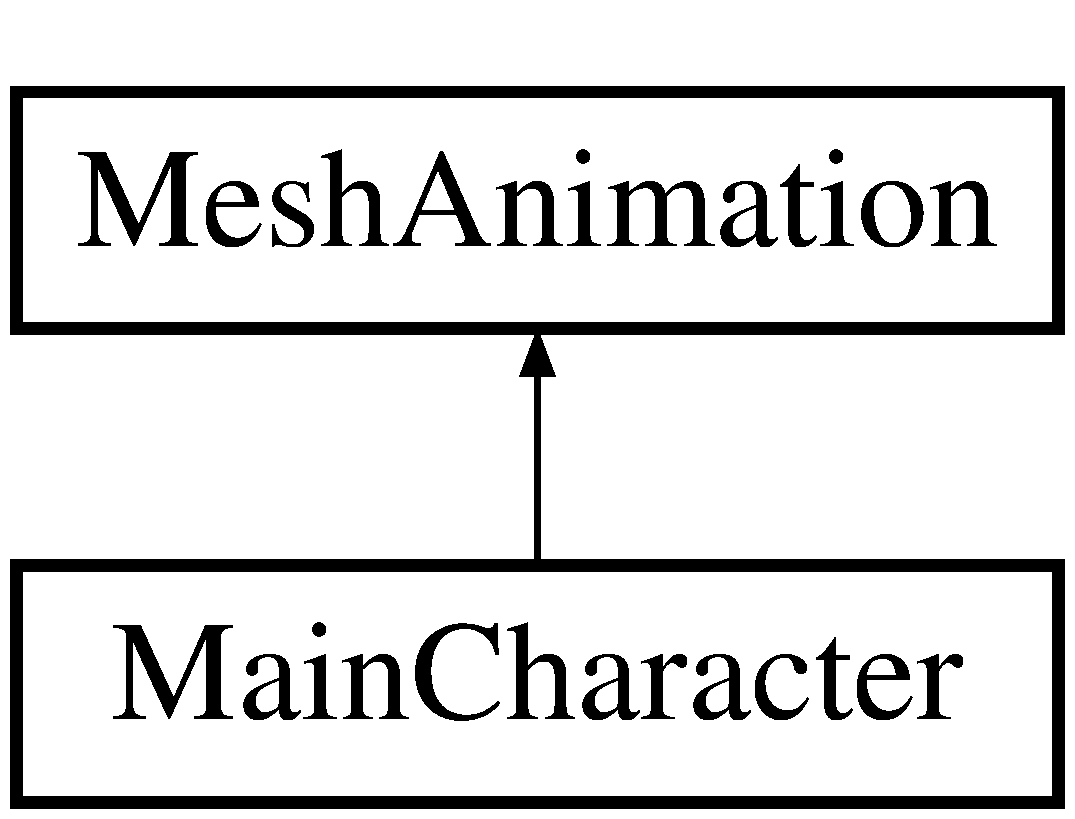
\includegraphics[height=2.000000cm]{class_main_character}
\end{center}
\end{figure}
\subsection*{Public Member Functions}
\begin{DoxyCompactItemize}
\item 
\hyperlink{class_main_character_ad9fb34855d2ba64910e20410c8e0c6ec}{Main\-Character} (const char $\ast$filename, \hyperlink{class_camera}{Camera} $\ast$\hyperlink{class_main_character_aed23e5d05c1fb771c303d4f3e180aa66}{camera})
\begin{DoxyCompactList}\small\item\em Constructor hardcodat -\/ T\-O\-D\-O generalizare. \end{DoxyCompactList}\item 
\hyperlink{class_main_character_a6d7d97ce443fa977a798ea1c956b0fc1}{$\sim$\-Main\-Character} ()
\item 
virtual void \hyperlink{class_main_character_adf0f10646b7e00949b7a594cbc161c64}{render} (std\-::vector$<$ \hyperlink{structobject}{object} $>$ \&comp, float $\ast$buffer, float $\ast$restore\-\_\-buffer)
\begin{DoxyCompactList}\small\item\em deseneaza personajul animat \end{DoxyCompactList}\item 
void \hyperlink{class_main_character_a5f57b318af6b7919ad7594603a35750c}{reset} ()
\begin{DoxyCompactList}\small\item\em reseteaza pozitia, rotatia personajului la cele initiale \end{DoxyCompactList}\item 
virtual void \hyperlink{class_main_character_aa5ae776c23b6f09beae33ac3ad015add}{save\-State} ()
\begin{DoxyCompactList}\small\item\em Uncompleted -\/ T\-O\-D\-O. \end{DoxyCompactList}\item 
virtual void \hyperlink{class_main_character_ad37c1d914626650e7d77b9d8ae58b4a5}{load\-State} ()
\begin{DoxyCompactList}\small\item\em Salveaza starea curenta a jocului. \end{DoxyCompactList}\item 
virtual float $\ast$ \hyperlink{class_main_character_a2615c112f8784972fa57b0c585a52ca8}{wrap\-Bounding\-Box} (\hyperlink{struct_vector3}{Vector3} \&request\-\_\-poz, int \&inx, int id)
\begin{DoxyCompactList}\small\item\em Transforma bounding-\/box-\/ul intr-\/un vector de float-\/uri. A se vedea protocolul client-\/ server. \end{DoxyCompactList}\item 
void \hyperlink{class_main_character_a8664ab320c6d2e258143119a03b7458f}{resolve\-\_\-collision} (float $\ast$wanted\-\_\-pos, float $\ast$results)
\begin{DoxyCompactList}\small\item\em ajusteaza pozitia personajului dupa rezultatele coliziunii -\/ uncompleted T\-O\-D\-O \end{DoxyCompactList}\item 
void \hyperlink{class_main_character_a0886ea364317c67aa139d6f3d25d69b5}{send\-Buffers} (float $\ast$buffer\-\_\-wanted, float $\ast$buffer\-\_\-restore)
\begin{DoxyCompactList}\small\item\em Trimite buffer-\/ul cu bounding-\/box-\/ul spre server. \end{DoxyCompactList}\end{DoxyCompactItemize}
\subsection*{Public Attributes}
\begin{DoxyCompactItemize}
\item 
\hyperlink{class_camera}{Camera} $\ast$ \hyperlink{class_main_character_aed23e5d05c1fb771c303d4f3e180aa66}{camera}
\item 
\hyperlink{struct_vector3}{Vector3} \hyperlink{class_main_character_ad8584e16c6e3f1b599fe9fad7511b14f}{position}
\item 
float \hyperlink{class_main_character_aa84b9f2c698f1247c8d95a60105cdbb7}{orientation}
\end{DoxyCompactItemize}


\subsection{Detailed Description}


Definition at line 124 of file static\-Obj.\-h.



\subsection{Constructor \& Destructor Documentation}
\hypertarget{class_main_character_ad9fb34855d2ba64910e20410c8e0c6ec}{\index{Main\-Character@{Main\-Character}!Main\-Character@{Main\-Character}}
\index{Main\-Character@{Main\-Character}!MainCharacter@{Main\-Character}}
\subsubsection[{Main\-Character}]{\setlength{\rightskip}{0pt plus 5cm}Main\-Character\-::\-Main\-Character (
\begin{DoxyParamCaption}
\item[{const char $\ast$}]{filename, }
\item[{{\bf Camera} $\ast$}]{camera}
\end{DoxyParamCaption}
)}}\label{class_main_character_ad9fb34855d2ba64910e20410c8e0c6ec}


Constructor hardcodat -\/ T\-O\-D\-O generalizare. 



Definition at line 349 of file static\-Obj.\-cpp.

\hypertarget{class_main_character_a6d7d97ce443fa977a798ea1c956b0fc1}{\index{Main\-Character@{Main\-Character}!$\sim$\-Main\-Character@{$\sim$\-Main\-Character}}
\index{$\sim$\-Main\-Character@{$\sim$\-Main\-Character}!MainCharacter@{Main\-Character}}
\subsubsection[{$\sim$\-Main\-Character}]{\setlength{\rightskip}{0pt plus 5cm}Main\-Character\-::$\sim$\-Main\-Character (
\begin{DoxyParamCaption}
{}
\end{DoxyParamCaption}
)}}\label{class_main_character_a6d7d97ce443fa977a798ea1c956b0fc1}


Definition at line 364 of file static\-Obj.\-cpp.



\subsection{Member Function Documentation}
\hypertarget{class_main_character_ad37c1d914626650e7d77b9d8ae58b4a5}{\index{Main\-Character@{Main\-Character}!load\-State@{load\-State}}
\index{load\-State@{load\-State}!MainCharacter@{Main\-Character}}
\subsubsection[{load\-State}]{\setlength{\rightskip}{0pt plus 5cm}void Main\-Character\-::load\-State (
\begin{DoxyParamCaption}
{}
\end{DoxyParamCaption}
)\hspace{0.3cm}{\ttfamily [virtual]}}}\label{class_main_character_ad37c1d914626650e7d77b9d8ae58b4a5}


Salveaza starea curenta a jocului. 



Definition at line 495 of file static\-Obj.\-cpp.

\hypertarget{class_main_character_adf0f10646b7e00949b7a594cbc161c64}{\index{Main\-Character@{Main\-Character}!render@{render}}
\index{render@{render}!MainCharacter@{Main\-Character}}
\subsubsection[{render}]{\setlength{\rightskip}{0pt plus 5cm}void Main\-Character\-::render (
\begin{DoxyParamCaption}
\item[{std\-::vector$<$ {\bf object} $>$ \&}]{comp, }
\item[{float $\ast$}]{buffer, }
\item[{float $\ast$}]{restore\-\_\-buffer}
\end{DoxyParamCaption}
)\hspace{0.3cm}{\ttfamily [virtual]}}}\label{class_main_character_adf0f10646b7e00949b7a594cbc161c64}


deseneaza personajul animat 



Reimplemented from \hyperlink{class_mesh_animation_ae64ddb4d27ebb9d64fe11b2e3143754e}{Mesh\-Animation}.



Definition at line 368 of file static\-Obj.\-cpp.

\hypertarget{class_main_character_a5f57b318af6b7919ad7594603a35750c}{\index{Main\-Character@{Main\-Character}!reset@{reset}}
\index{reset@{reset}!MainCharacter@{Main\-Character}}
\subsubsection[{reset}]{\setlength{\rightskip}{0pt plus 5cm}void Main\-Character\-::reset (
\begin{DoxyParamCaption}
{}
\end{DoxyParamCaption}
)}}\label{class_main_character_a5f57b318af6b7919ad7594603a35750c}


reseteaza pozitia, rotatia personajului la cele initiale 



Definition at line 468 of file static\-Obj.\-cpp.

\hypertarget{class_main_character_a8664ab320c6d2e258143119a03b7458f}{\index{Main\-Character@{Main\-Character}!resolve\-\_\-collision@{resolve\-\_\-collision}}
\index{resolve\-\_\-collision@{resolve\-\_\-collision}!MainCharacter@{Main\-Character}}
\subsubsection[{resolve\-\_\-collision}]{\setlength{\rightskip}{0pt plus 5cm}void Main\-Character\-::resolve\-\_\-collision (
\begin{DoxyParamCaption}
\item[{float $\ast$}]{wanted\-\_\-pos, }
\item[{float $\ast$}]{results}
\end{DoxyParamCaption}
)}}\label{class_main_character_a8664ab320c6d2e258143119a03b7458f}


ajusteaza pozitia personajului dupa rezultatele coliziunii -\/ uncompleted T\-O\-D\-O 



Definition at line 395 of file static\-Obj.\-cpp.

\hypertarget{class_main_character_aa5ae776c23b6f09beae33ac3ad015add}{\index{Main\-Character@{Main\-Character}!save\-State@{save\-State}}
\index{save\-State@{save\-State}!MainCharacter@{Main\-Character}}
\subsubsection[{save\-State}]{\setlength{\rightskip}{0pt plus 5cm}void Main\-Character\-::save\-State (
\begin{DoxyParamCaption}
{}
\end{DoxyParamCaption}
)\hspace{0.3cm}{\ttfamily [virtual]}}}\label{class_main_character_aa5ae776c23b6f09beae33ac3ad015add}


Uncompleted -\/ T\-O\-D\-O. 



Definition at line 476 of file static\-Obj.\-cpp.

\hypertarget{class_main_character_a0886ea364317c67aa139d6f3d25d69b5}{\index{Main\-Character@{Main\-Character}!send\-Buffers@{send\-Buffers}}
\index{send\-Buffers@{send\-Buffers}!MainCharacter@{Main\-Character}}
\subsubsection[{send\-Buffers}]{\setlength{\rightskip}{0pt plus 5cm}void Main\-Character\-::send\-Buffers (
\begin{DoxyParamCaption}
\item[{float $\ast$}]{buffer\-\_\-wanted, }
\item[{float $\ast$}]{buffer\-\_\-restore}
\end{DoxyParamCaption}
)}}\label{class_main_character_a0886ea364317c67aa139d6f3d25d69b5}


Trimite buffer-\/ul cu bounding-\/box-\/ul spre server. 

\hypertarget{class_main_character_a2615c112f8784972fa57b0c585a52ca8}{\index{Main\-Character@{Main\-Character}!wrap\-Bounding\-Box@{wrap\-Bounding\-Box}}
\index{wrap\-Bounding\-Box@{wrap\-Bounding\-Box}!MainCharacter@{Main\-Character}}
\subsubsection[{wrap\-Bounding\-Box}]{\setlength{\rightskip}{0pt plus 5cm}float $\ast$ Main\-Character\-::wrap\-Bounding\-Box (
\begin{DoxyParamCaption}
\item[{{\bf Vector3} \&}]{request\-\_\-poz, }
\item[{int \&}]{inx, }
\item[{int}]{id}
\end{DoxyParamCaption}
)\hspace{0.3cm}{\ttfamily [virtual]}}}\label{class_main_character_a2615c112f8784972fa57b0c585a52ca8}


Transforma bounding-\/box-\/ul intr-\/un vector de float-\/uri. A se vedea protocolul client-\/ server. 



Definition at line 434 of file static\-Obj.\-cpp.



\subsection{Member Data Documentation}
\hypertarget{class_main_character_aed23e5d05c1fb771c303d4f3e180aa66}{\index{Main\-Character@{Main\-Character}!camera@{camera}}
\index{camera@{camera}!MainCharacter@{Main\-Character}}
\subsubsection[{camera}]{\setlength{\rightskip}{0pt plus 5cm}{\bf Camera}$\ast$ Main\-Character\-::camera}}\label{class_main_character_aed23e5d05c1fb771c303d4f3e180aa66}


Definition at line 126 of file static\-Obj.\-h.

\hypertarget{class_main_character_aa84b9f2c698f1247c8d95a60105cdbb7}{\index{Main\-Character@{Main\-Character}!orientation@{orientation}}
\index{orientation@{orientation}!MainCharacter@{Main\-Character}}
\subsubsection[{orientation}]{\setlength{\rightskip}{0pt plus 5cm}float Main\-Character\-::orientation}}\label{class_main_character_aa84b9f2c698f1247c8d95a60105cdbb7}

\begin{DoxyParams}{Parameters}
{\em orientation} & -\/ unghiul in jurul axei y \\
\hline
\end{DoxyParams}


Definition at line 134 of file static\-Obj.\-h.

\hypertarget{class_main_character_ad8584e16c6e3f1b599fe9fad7511b14f}{\index{Main\-Character@{Main\-Character}!position@{position}}
\index{position@{position}!MainCharacter@{Main\-Character}}
\subsubsection[{position}]{\setlength{\rightskip}{0pt plus 5cm}{\bf Vector3} Main\-Character\-::position}}\label{class_main_character_ad8584e16c6e3f1b599fe9fad7511b14f}

\begin{DoxyParams}{Parameters}
{\em -\/} & position pozitia la care se afla personajul \\
\hline
\end{DoxyParams}


Definition at line 130 of file static\-Obj.\-h.



The documentation for this class was generated from the following files\-:\begin{DoxyCompactItemize}
\item 
\hyperlink{static_obj_8h}{static\-Obj.\-h}\item 
\hyperlink{static_obj_8cpp}{static\-Obj.\-cpp}\end{DoxyCompactItemize}

\hypertarget{class_main_c_haracter}{\section{Main\-C\-Haracter Class Reference}
\label{class_main_c_haracter}\index{Main\-C\-Haracter@{Main\-C\-Haracter}}
}


\subsection{Detailed Description}
personajului urmarit de camera 

The documentation for this class was generated from the following file\-:\begin{DoxyCompactItemize}
\item 
\hyperlink{static_obj_8h}{static\-Obj.\-h}\end{DoxyCompactItemize}

\hypertarget{class_mechanics_engine}{\section{Mechanics\-Engine Class Reference}
\label{class_mechanics_engine}\index{Mechanics\-Engine@{Mechanics\-Engine}}
}


{\ttfamily \#include $<$physic\-Engine.\-h$>$}

\subsection*{Static Public Member Functions}
\begin{DoxyCompactItemize}
\item 
static \hyperlink{struct_vector3}{Vector3} \hyperlink{class_mechanics_engine_adb51c3ca801460f0ed48b3a293ac72b3}{get\-Collisiton\-Directions} (\hyperlink{struct_vector3}{Vector3} \&dir1, float m1, \hyperlink{struct_vector3}{Vector3} \&dir2, float m2)
\begin{DoxyCompactList}\small\item\em returneaza directia unui obiect cu viteza \end{DoxyCompactList}\end{DoxyCompactItemize}


\subsection{Detailed Description}
sunt metodele care fac calcule de fizica 

Definition at line 10 of file physic\-Engine.\-h.



\subsection{Member Function Documentation}
\hypertarget{class_mechanics_engine_adb51c3ca801460f0ed48b3a293ac72b3}{\index{Mechanics\-Engine@{Mechanics\-Engine}!get\-Collisiton\-Directions@{get\-Collisiton\-Directions}}
\index{get\-Collisiton\-Directions@{get\-Collisiton\-Directions}!MechanicsEngine@{Mechanics\-Engine}}
\subsubsection[{get\-Collisiton\-Directions}]{\setlength{\rightskip}{0pt plus 5cm}{\bf Vector3} Mechanics\-Engine\-::get\-Collisiton\-Directions (
\begin{DoxyParamCaption}
\item[{{\bf Vector3} \&}]{dir1, }
\item[{float}]{m1, }
\item[{{\bf Vector3} \&}]{dir2, }
\item[{float}]{m2}
\end{DoxyParamCaption}
)\hspace{0.3cm}{\ttfamily [static]}}}\label{class_mechanics_engine_adb51c3ca801460f0ed48b3a293ac72b3}


returneaza directia unui obiect cu viteza 


\begin{DoxyParams}{Parameters}
{\em dir1,masa} & \\
\hline
{\em m1,cand} & se ciocneste cu obiectul de directie \\
\hline
{\em dir2} & si masa \\
\hline
{\em m2} & \\
\hline
\end{DoxyParams}


Definition at line 4 of file physic\-Engine.\-cpp.



The documentation for this class was generated from the following files\-:\begin{DoxyCompactItemize}
\item 
\hyperlink{physic_engine_8h}{physic\-Engine.\-h}\item 
\hyperlink{physic_engine_8cpp}{physic\-Engine.\-cpp}\end{DoxyCompactItemize}

\hypertarget{class_menu_g_u_i}{\section{Menu\-G\-U\-I Class Reference}
\label{class_menu_g_u_i}\index{Menu\-G\-U\-I@{Menu\-G\-U\-I}}
}


{\ttfamily \#include $<$Menu\-G\-U\-I.\-h$>$}

\subsection*{Public Member Functions}
\begin{DoxyCompactItemize}
\item 
\hyperlink{class_menu_g_u_i_a2c41412095fc43e66c6acceb664a203c}{Menu\-G\-U\-I} ()
\item 
\hyperlink{class_menu_g_u_i_ade7e3f7fb26b4a0befb4cb3e0bf30cee}{$\sim$\-Menu\-G\-U\-I} ()
\item 
void \hyperlink{class_menu_g_u_i_abc57c1997de32e0c17713f9d20728186}{display} ()
\begin{DoxyCompactList}\small\item\em deseneaza meniul pe ecran \end{DoxyCompactList}\item 
void \hyperlink{class_menu_g_u_i_ae2a838fa10f38966e49580494057d25c}{bind\-Texture} ()
\begin{DoxyCompactList}\small\item\em Din cauza faptului ca se genereaza o textura noua de fiecare data cand se intra in meniu, trebuie legata textura noua de fiecare data. \end{DoxyCompactList}\item 
void \hyperlink{class_menu_g_u_i_a98ea7d1a53b4f583ead229f80b872ff5}{delete\-Texture} ()
\item 
void \hyperlink{class_menu_g_u_i_ad1fba8bb6d1851e4ab663ca869275162}{show} ()
\begin{DoxyCompactList}\small\item\em Arata meni-\/ul, cam la fel ca si interfata din Java. \end{DoxyCompactList}\item 
void \hyperlink{class_menu_g_u_i_ab86e29450e7bf0ded4f41213658f9291}{hide} ()
\begin{DoxyCompactList}\small\item\em Ascunde meniul sau mai bine zis impiedica desenarea acestuia pe ecran. \end{DoxyCompactList}\item 
bool \hyperlink{class_menu_g_u_i_a1a87191bece0e81a6fdbc0ea9fc1b823}{is\-Visible} () const 
\item 
void \hyperlink{class_menu_g_u_i_ab94886a43e3598ce490116bd06f3c828}{selective\-Blur} (unsigned char $\ast$original\-Img)
\begin{DoxyCompactList}\small\item\em Calculeaza efectul imaginii de fundal. \end{DoxyCompactList}\end{DoxyCompactItemize}
\subsection*{Public Attributes}
\begin{DoxyCompactItemize}
\item 
\hyperlink{structobject}{object} \hyperlink{class_menu_g_u_i_a5f70990c15a161d6d9e04e436599e59c}{bkg\-\_\-obj}
\item 
\hyperlink{structobject}{object} \hyperlink{class_menu_g_u_i_a04d8a13b8437fa0ae19d5913f18678e3}{logo}
\item 
std\-::vector$<$ \hyperlink{structobject}{object} $>$ \hyperlink{class_menu_g_u_i_afb740b4478b7214db49bcfb8bca4350d}{menu\-\_\-list}
\item 
std\-::vector$<$ \hyperlink{structobject}{object} $>$ \hyperlink{class_menu_g_u_i_a2f433c33f8a0e3e6e37b79b6fb0dc57d}{dialog\-\_\-list}
\item 
int \hyperlink{class_menu_g_u_i_a6e978784cb9e9792dd96d935f9a2d1ca}{selected}
\item 
volatile int \hyperlink{class_menu_g_u_i_a16ac33cf65fbb4ce84e076a71aeb6137}{screen\-Width}
\item 
volatile int \hyperlink{class_menu_g_u_i_a41dee14f0233c0a7159f0601b3016e3a}{screen\-Height}
\item 
bool \hyperlink{class_menu_g_u_i_aeb5b730a3faea08895e234e1ad9ab53d}{visible}
\end{DoxyCompactItemize}


\subsection{Detailed Description}
pentru meniul aplicatiei Contine butoane, cutii de dialog, background, logo 

Definition at line 11 of file Menu\-G\-U\-I.\-h.



\subsection{Constructor \& Destructor Documentation}
\hypertarget{class_menu_g_u_i_a2c41412095fc43e66c6acceb664a203c}{\index{Menu\-G\-U\-I@{Menu\-G\-U\-I}!Menu\-G\-U\-I@{Menu\-G\-U\-I}}
\index{Menu\-G\-U\-I@{Menu\-G\-U\-I}!MenuGUI@{Menu\-G\-U\-I}}
\subsubsection[{Menu\-G\-U\-I}]{\setlength{\rightskip}{0pt plus 5cm}Menu\-G\-U\-I\-::\-Menu\-G\-U\-I (
\begin{DoxyParamCaption}
{}
\end{DoxyParamCaption}
)}}\label{class_menu_g_u_i_a2c41412095fc43e66c6acceb664a203c}


Definition at line 3 of file Menu\-G\-U\-I.\-cpp.

\hypertarget{class_menu_g_u_i_ade7e3f7fb26b4a0befb4cb3e0bf30cee}{\index{Menu\-G\-U\-I@{Menu\-G\-U\-I}!$\sim$\-Menu\-G\-U\-I@{$\sim$\-Menu\-G\-U\-I}}
\index{$\sim$\-Menu\-G\-U\-I@{$\sim$\-Menu\-G\-U\-I}!MenuGUI@{Menu\-G\-U\-I}}
\subsubsection[{$\sim$\-Menu\-G\-U\-I}]{\setlength{\rightskip}{0pt plus 5cm}Menu\-G\-U\-I\-::$\sim$\-Menu\-G\-U\-I (
\begin{DoxyParamCaption}
{}
\end{DoxyParamCaption}
)}}\label{class_menu_g_u_i_ade7e3f7fb26b4a0befb4cb3e0bf30cee}


Definition at line 56 of file Menu\-G\-U\-I.\-cpp.



\subsection{Member Function Documentation}
\hypertarget{class_menu_g_u_i_ae2a838fa10f38966e49580494057d25c}{\index{Menu\-G\-U\-I@{Menu\-G\-U\-I}!bind\-Texture@{bind\-Texture}}
\index{bind\-Texture@{bind\-Texture}!MenuGUI@{Menu\-G\-U\-I}}
\subsubsection[{bind\-Texture}]{\setlength{\rightskip}{0pt plus 5cm}void Menu\-G\-U\-I\-::bind\-Texture (
\begin{DoxyParamCaption}
{}
\end{DoxyParamCaption}
)}}\label{class_menu_g_u_i_ae2a838fa10f38966e49580494057d25c}


Din cauza faptului ca se genereaza o textura noua de fiecare data cand se intra in meniu, trebuie legata textura noua de fiecare data. 



Definition at line 60 of file Menu\-G\-U\-I.\-cpp.

\hypertarget{class_menu_g_u_i_a98ea7d1a53b4f583ead229f80b872ff5}{\index{Menu\-G\-U\-I@{Menu\-G\-U\-I}!delete\-Texture@{delete\-Texture}}
\index{delete\-Texture@{delete\-Texture}!MenuGUI@{Menu\-G\-U\-I}}
\subsubsection[{delete\-Texture}]{\setlength{\rightskip}{0pt plus 5cm}void Menu\-G\-U\-I\-::delete\-Texture (
\begin{DoxyParamCaption}
{}
\end{DoxyParamCaption}
)}}\label{class_menu_g_u_i_a98ea7d1a53b4f583ead229f80b872ff5}
sterge textura dupa ce nu mai este folosita 

Definition at line 87 of file Menu\-G\-U\-I.\-cpp.

\hypertarget{class_menu_g_u_i_abc57c1997de32e0c17713f9d20728186}{\index{Menu\-G\-U\-I@{Menu\-G\-U\-I}!display@{display}}
\index{display@{display}!MenuGUI@{Menu\-G\-U\-I}}
\subsubsection[{display}]{\setlength{\rightskip}{0pt plus 5cm}void Menu\-G\-U\-I\-::display (
\begin{DoxyParamCaption}
{}
\end{DoxyParamCaption}
)}}\label{class_menu_g_u_i_abc57c1997de32e0c17713f9d20728186}


deseneaza meniul pe ecran 



Definition at line 93 of file Menu\-G\-U\-I.\-cpp.

\hypertarget{class_menu_g_u_i_ab86e29450e7bf0ded4f41213658f9291}{\index{Menu\-G\-U\-I@{Menu\-G\-U\-I}!hide@{hide}}
\index{hide@{hide}!MenuGUI@{Menu\-G\-U\-I}}
\subsubsection[{hide}]{\setlength{\rightskip}{0pt plus 5cm}void Menu\-G\-U\-I\-::hide (
\begin{DoxyParamCaption}
{}
\end{DoxyParamCaption}
)\hspace{0.3cm}{\ttfamily [inline]}}}\label{class_menu_g_u_i_ab86e29450e7bf0ded4f41213658f9291}


Ascunde meniul sau mai bine zis impiedica desenarea acestuia pe ecran. 



Definition at line 53 of file Menu\-G\-U\-I.\-h.

\hypertarget{class_menu_g_u_i_a1a87191bece0e81a6fdbc0ea9fc1b823}{\index{Menu\-G\-U\-I@{Menu\-G\-U\-I}!is\-Visible@{is\-Visible}}
\index{is\-Visible@{is\-Visible}!MenuGUI@{Menu\-G\-U\-I}}
\subsubsection[{is\-Visible}]{\setlength{\rightskip}{0pt plus 5cm}bool Menu\-G\-U\-I\-::is\-Visible (
\begin{DoxyParamCaption}
{}
\end{DoxyParamCaption}
) const\hspace{0.3cm}{\ttfamily [inline]}}}\label{class_menu_g_u_i_a1a87191bece0e81a6fdbc0ea9fc1b823}
\begin{DoxyReturn}{Returns}
Returneaza daca sau nu meniul este vizibil 
\end{DoxyReturn}


Definition at line 58 of file Menu\-G\-U\-I.\-h.

\hypertarget{class_menu_g_u_i_ab94886a43e3598ce490116bd06f3c828}{\index{Menu\-G\-U\-I@{Menu\-G\-U\-I}!selective\-Blur@{selective\-Blur}}
\index{selective\-Blur@{selective\-Blur}!MenuGUI@{Menu\-G\-U\-I}}
\subsubsection[{selective\-Blur}]{\setlength{\rightskip}{0pt plus 5cm}void Menu\-G\-U\-I\-::selective\-Blur (
\begin{DoxyParamCaption}
\item[{unsigned char $\ast$}]{original\-Img}
\end{DoxyParamCaption}
)}}\label{class_menu_g_u_i_ab94886a43e3598ce490116bd06f3c828}


Calculeaza efectul imaginii de fundal. 



Definition at line 137 of file Menu\-G\-U\-I.\-cpp.

\hypertarget{class_menu_g_u_i_ad1fba8bb6d1851e4ab663ca869275162}{\index{Menu\-G\-U\-I@{Menu\-G\-U\-I}!show@{show}}
\index{show@{show}!MenuGUI@{Menu\-G\-U\-I}}
\subsubsection[{show}]{\setlength{\rightskip}{0pt plus 5cm}void Menu\-G\-U\-I\-::show (
\begin{DoxyParamCaption}
{}
\end{DoxyParamCaption}
)\hspace{0.3cm}{\ttfamily [inline]}}}\label{class_menu_g_u_i_ad1fba8bb6d1851e4ab663ca869275162}


Arata meni-\/ul, cam la fel ca si interfata din Java. 



Definition at line 43 of file Menu\-G\-U\-I.\-h.



\subsection{Member Data Documentation}
\hypertarget{class_menu_g_u_i_a5f70990c15a161d6d9e04e436599e59c}{\index{Menu\-G\-U\-I@{Menu\-G\-U\-I}!bkg\-\_\-obj@{bkg\-\_\-obj}}
\index{bkg\-\_\-obj@{bkg\-\_\-obj}!MenuGUI@{Menu\-G\-U\-I}}
\subsubsection[{bkg\-\_\-obj}]{\setlength{\rightskip}{0pt plus 5cm}{\bf object} Menu\-G\-U\-I\-::bkg\-\_\-obj}}\label{class_menu_g_u_i_a5f70990c15a161d6d9e04e436599e59c}


Definition at line 13 of file Menu\-G\-U\-I.\-h.

\hypertarget{class_menu_g_u_i_a2f433c33f8a0e3e6e37b79b6fb0dc57d}{\index{Menu\-G\-U\-I@{Menu\-G\-U\-I}!dialog\-\_\-list@{dialog\-\_\-list}}
\index{dialog\-\_\-list@{dialog\-\_\-list}!MenuGUI@{Menu\-G\-U\-I}}
\subsubsection[{dialog\-\_\-list}]{\setlength{\rightskip}{0pt plus 5cm}std\-::vector$<${\bf object}$>$ Menu\-G\-U\-I\-::dialog\-\_\-list}}\label{class_menu_g_u_i_a2f433c33f8a0e3e6e37b79b6fb0dc57d}


Definition at line 16 of file Menu\-G\-U\-I.\-h.

\hypertarget{class_menu_g_u_i_a04d8a13b8437fa0ae19d5913f18678e3}{\index{Menu\-G\-U\-I@{Menu\-G\-U\-I}!logo@{logo}}
\index{logo@{logo}!MenuGUI@{Menu\-G\-U\-I}}
\subsubsection[{logo}]{\setlength{\rightskip}{0pt plus 5cm}{\bf object} Menu\-G\-U\-I\-::logo}}\label{class_menu_g_u_i_a04d8a13b8437fa0ae19d5913f18678e3}


Definition at line 14 of file Menu\-G\-U\-I.\-h.

\hypertarget{class_menu_g_u_i_afb740b4478b7214db49bcfb8bca4350d}{\index{Menu\-G\-U\-I@{Menu\-G\-U\-I}!menu\-\_\-list@{menu\-\_\-list}}
\index{menu\-\_\-list@{menu\-\_\-list}!MenuGUI@{Menu\-G\-U\-I}}
\subsubsection[{menu\-\_\-list}]{\setlength{\rightskip}{0pt plus 5cm}std\-::vector$<${\bf object}$>$ Menu\-G\-U\-I\-::menu\-\_\-list}}\label{class_menu_g_u_i_afb740b4478b7214db49bcfb8bca4350d}


Definition at line 15 of file Menu\-G\-U\-I.\-h.

\hypertarget{class_menu_g_u_i_a41dee14f0233c0a7159f0601b3016e3a}{\index{Menu\-G\-U\-I@{Menu\-G\-U\-I}!screen\-Height@{screen\-Height}}
\index{screen\-Height@{screen\-Height}!MenuGUI@{Menu\-G\-U\-I}}
\subsubsection[{screen\-Height}]{\setlength{\rightskip}{0pt plus 5cm}volatile int Menu\-G\-U\-I\-::screen\-Height}}\label{class_menu_g_u_i_a41dee14f0233c0a7159f0601b3016e3a}


Definition at line 18 of file Menu\-G\-U\-I.\-h.

\hypertarget{class_menu_g_u_i_a16ac33cf65fbb4ce84e076a71aeb6137}{\index{Menu\-G\-U\-I@{Menu\-G\-U\-I}!screen\-Width@{screen\-Width}}
\index{screen\-Width@{screen\-Width}!MenuGUI@{Menu\-G\-U\-I}}
\subsubsection[{screen\-Width}]{\setlength{\rightskip}{0pt plus 5cm}volatile int Menu\-G\-U\-I\-::screen\-Width}}\label{class_menu_g_u_i_a16ac33cf65fbb4ce84e076a71aeb6137}


Definition at line 18 of file Menu\-G\-U\-I.\-h.

\hypertarget{class_menu_g_u_i_a6e978784cb9e9792dd96d935f9a2d1ca}{\index{Menu\-G\-U\-I@{Menu\-G\-U\-I}!selected@{selected}}
\index{selected@{selected}!MenuGUI@{Menu\-G\-U\-I}}
\subsubsection[{selected}]{\setlength{\rightskip}{0pt plus 5cm}int Menu\-G\-U\-I\-::selected}}\label{class_menu_g_u_i_a6e978784cb9e9792dd96d935f9a2d1ca}


Definition at line 17 of file Menu\-G\-U\-I.\-h.

\hypertarget{class_menu_g_u_i_aeb5b730a3faea08895e234e1ad9ab53d}{\index{Menu\-G\-U\-I@{Menu\-G\-U\-I}!visible@{visible}}
\index{visible@{visible}!MenuGUI@{Menu\-G\-U\-I}}
\subsubsection[{visible}]{\setlength{\rightskip}{0pt plus 5cm}bool Menu\-G\-U\-I\-::visible}}\label{class_menu_g_u_i_aeb5b730a3faea08895e234e1ad9ab53d}


Definition at line 19 of file Menu\-G\-U\-I.\-h.



The documentation for this class was generated from the following files\-:\begin{DoxyCompactItemize}
\item 
\hyperlink{_menu_g_u_i_8h}{Menu\-G\-U\-I.\-h}\item 
\hyperlink{_menu_g_u_i_8cpp}{Menu\-G\-U\-I.\-cpp}\end{DoxyCompactItemize}

\hypertarget{class_mesh_animation}{\section{Mesh\-Animation Class Reference}
\label{class_mesh_animation}\index{Mesh\-Animation@{Mesh\-Animation}}
}


{\ttfamily \#include $<$static\-Obj.\-h$>$}

Inheritance diagram for Mesh\-Animation\-:\begin{figure}[H]
\begin{center}
\leavevmode
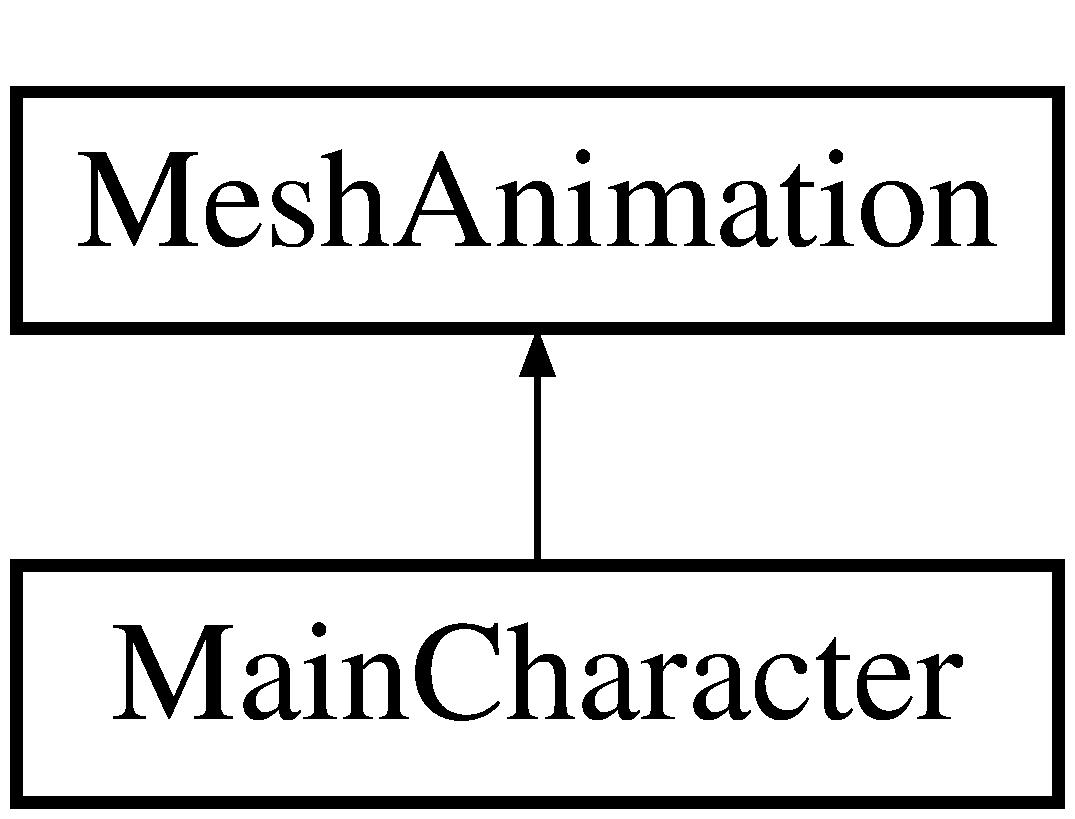
\includegraphics[height=2.000000cm]{class_mesh_animation}
\end{center}
\end{figure}
\subsection*{Public Member Functions}
\begin{DoxyCompactItemize}
\item 
\hyperlink{class_mesh_animation_a567a0c3da9b6ab4f8731ca9a2d292122}{Mesh\-Animation} (const char $\ast$filename, int frame\-\_\-no)
\item 
\hyperlink{class_mesh_animation_ab5b3efcd554bf01b8fd04120fc93c8df}{$\sim$\-Mesh\-Animation} ()
\item 
virtual void \hyperlink{class_mesh_animation_ae64ddb4d27ebb9d64fe11b2e3143754e}{render} (std\-::vector$<$ \hyperlink{structobject}{object} $>$ \&comp, float $\ast$buffer, float $\ast$restore\-\_\-buffer)
\begin{DoxyCompactList}\small\item\em Deseneaza frame-\/ul corect al animatiei. \end{DoxyCompactList}\end{DoxyCompactItemize}
\subsection*{Public Attributes}
\begin{DoxyCompactItemize}
\item 
std\-::vector$<$ \hyperlink{structobject}{object} $>$ \hyperlink{class_mesh_animation_a925b14f1959e8978bf2381cae04faddc}{frames}
\item 
std\-::vector$<$ \hyperlink{struct_move}{Move} $>$ \hyperlink{class_mesh_animation_a143c0f0b32676ba0cc63c5596f129b21}{moves}
\item 
int \hyperlink{class_mesh_animation_a38be50473060fbf1433104c3ebf4dda6}{current\-\_\-frame\-\_\-no}
\item 
\hyperlink{struct_move}{Move} \hyperlink{class_mesh_animation_a0e99877081ae52a2b74d890a346a5298}{current\-\_\-move}
\end{DoxyCompactItemize}


\subsection{Detailed Description}
obiect animat 

Definition at line 83 of file static\-Obj.\-h.



\subsection{Constructor \& Destructor Documentation}
\hypertarget{class_mesh_animation_a567a0c3da9b6ab4f8731ca9a2d292122}{\index{Mesh\-Animation@{Mesh\-Animation}!Mesh\-Animation@{Mesh\-Animation}}
\index{Mesh\-Animation@{Mesh\-Animation}!MeshAnimation@{Mesh\-Animation}}
\subsubsection[{Mesh\-Animation}]{\setlength{\rightskip}{0pt plus 5cm}Mesh\-Animation\-::\-Mesh\-Animation (
\begin{DoxyParamCaption}
\item[{const char $\ast$}]{filename, }
\item[{int}]{frame\-\_\-no}
\end{DoxyParamCaption}
)}}\label{class_mesh_animation_a567a0c3da9b6ab4f8731ca9a2d292122}

\begin{DoxyParams}{Parameters}
{\em filename} & -\/ prefix-\/ul din nume comun tuturor frame-\/urilor Frame-\/urile sunt citite din fisiere .obj \\
\hline
{\em frame-\/no} & -\/ numarul de frame-\/uri \\
\hline
\end{DoxyParams}


Definition at line 307 of file static\-Obj.\-cpp.

\hypertarget{class_mesh_animation_ab5b3efcd554bf01b8fd04120fc93c8df}{\index{Mesh\-Animation@{Mesh\-Animation}!$\sim$\-Mesh\-Animation@{$\sim$\-Mesh\-Animation}}
\index{$\sim$\-Mesh\-Animation@{$\sim$\-Mesh\-Animation}!MeshAnimation@{Mesh\-Animation}}
\subsubsection[{$\sim$\-Mesh\-Animation}]{\setlength{\rightskip}{0pt plus 5cm}Mesh\-Animation\-::$\sim$\-Mesh\-Animation (
\begin{DoxyParamCaption}
{}
\end{DoxyParamCaption}
)}}\label{class_mesh_animation_ab5b3efcd554bf01b8fd04120fc93c8df}


Definition at line 337 of file static\-Obj.\-cpp.



\subsection{Member Function Documentation}
\hypertarget{class_mesh_animation_ae64ddb4d27ebb9d64fe11b2e3143754e}{\index{Mesh\-Animation@{Mesh\-Animation}!render@{render}}
\index{render@{render}!MeshAnimation@{Mesh\-Animation}}
\subsubsection[{render}]{\setlength{\rightskip}{0pt plus 5cm}void Mesh\-Animation\-::render (
\begin{DoxyParamCaption}
\item[{std\-::vector$<$ {\bf object} $>$ \&}]{comp, }
\item[{float $\ast$}]{buffer, }
\item[{float $\ast$}]{restore\-\_\-buffer}
\end{DoxyParamCaption}
)\hspace{0.3cm}{\ttfamily [virtual]}}}\label{class_mesh_animation_ae64ddb4d27ebb9d64fe11b2e3143754e}


Deseneaza frame-\/ul corect al animatiei. 



Reimplemented in \hyperlink{class_main_character_adf0f10646b7e00949b7a594cbc161c64}{Main\-Character}.



Definition at line 341 of file static\-Obj.\-cpp.



\subsection{Member Data Documentation}
\hypertarget{class_mesh_animation_a38be50473060fbf1433104c3ebf4dda6}{\index{Mesh\-Animation@{Mesh\-Animation}!current\-\_\-frame\-\_\-no@{current\-\_\-frame\-\_\-no}}
\index{current\-\_\-frame\-\_\-no@{current\-\_\-frame\-\_\-no}!MeshAnimation@{Mesh\-Animation}}
\subsubsection[{current\-\_\-frame\-\_\-no}]{\setlength{\rightskip}{0pt plus 5cm}int Mesh\-Animation\-::current\-\_\-frame\-\_\-no}}\label{class_mesh_animation_a38be50473060fbf1433104c3ebf4dda6}

\begin{DoxyParams}{Parameters}
{\em current\-\_\-frame\-\_\-no} & -\/ frame-\/ul curent la care se afla animatia in cadrul miscarii \\
\hline
\end{DoxyParams}


Definition at line 100 of file static\-Obj.\-h.

\hypertarget{class_mesh_animation_a0e99877081ae52a2b74d890a346a5298}{\index{Mesh\-Animation@{Mesh\-Animation}!current\-\_\-move@{current\-\_\-move}}
\index{current\-\_\-move@{current\-\_\-move}!MeshAnimation@{Mesh\-Animation}}
\subsubsection[{current\-\_\-move}]{\setlength{\rightskip}{0pt plus 5cm}{\bf Move} Mesh\-Animation\-::current\-\_\-move}}\label{class_mesh_animation_a0e99877081ae52a2b74d890a346a5298}

\begin{DoxyParams}{Parameters}
{\em current\-\_\-move} & -\/ miscara curenta a animatiei \\
\hline
\end{DoxyParams}


Definition at line 105 of file static\-Obj.\-h.

\hypertarget{class_mesh_animation_a925b14f1959e8978bf2381cae04faddc}{\index{Mesh\-Animation@{Mesh\-Animation}!frames@{frames}}
\index{frames@{frames}!MeshAnimation@{Mesh\-Animation}}
\subsubsection[{frames}]{\setlength{\rightskip}{0pt plus 5cm}std\-::vector$<${\bf object}$>$ Mesh\-Animation\-::frames}}\label{class_mesh_animation_a925b14f1959e8978bf2381cae04faddc}

\begin{DoxyParams}{Parameters}
{\em este} & un vector de mesh-\/uri care reprezinta frame-\/urile \\
\hline
\end{DoxyParams}


Definition at line 89 of file static\-Obj.\-h.

\hypertarget{class_mesh_animation_a143c0f0b32676ba0cc63c5596f129b21}{\index{Mesh\-Animation@{Mesh\-Animation}!moves@{moves}}
\index{moves@{moves}!MeshAnimation@{Mesh\-Animation}}
\subsubsection[{moves}]{\setlength{\rightskip}{0pt plus 5cm}std\-::vector$<${\bf Move}$>$ Mesh\-Animation\-::moves}}\label{class_mesh_animation_a143c0f0b32676ba0cc63c5596f129b21}

\begin{DoxyParams}{Parameters}
{\em moves} & este vectorul cu miscarile disponibile \\
\hline
\end{DoxyParams}


Definition at line 94 of file static\-Obj.\-h.



The documentation for this class was generated from the following files\-:\begin{DoxyCompactItemize}
\item 
\hyperlink{static_obj_8h}{static\-Obj.\-h}\item 
\hyperlink{static_obj_8cpp}{static\-Obj.\-cpp}\end{DoxyCompactItemize}

\hypertarget{struct_move}{\section{Move Struct Reference}
\label{struct_move}\index{Move@{Move}}
}


{\ttfamily \#include $<$static\-Obj.\-h$>$}

\subsection*{Public Attributes}
\begin{DoxyCompactItemize}
\item 
int \hyperlink{struct_move_a2e80ecb75dadd8a07adac3180805b122}{start}
\item 
int \hyperlink{struct_move_ab71b6eff5c90aa7fb96fc4509fd5e9b4}{length}
\end{DoxyCompactItemize}


\subsection{Detailed Description}
din miscarile animatiei 
\begin{DoxyParams}{Parameters}
{\em start} & reprezinta offset-\/ul in vectorul de frame-\/uri, iar length cate frame-\/uri are miscarea \\
\hline
\end{DoxyParams}


Definition at line 75 of file static\-Obj.\-h.



\subsection{Member Data Documentation}
\hypertarget{struct_move_ab71b6eff5c90aa7fb96fc4509fd5e9b4}{\index{Move@{Move}!length@{length}}
\index{length@{length}!Move@{Move}}
\subsubsection[{length}]{\setlength{\rightskip}{0pt plus 5cm}int Move\-::length}}\label{struct_move_ab71b6eff5c90aa7fb96fc4509fd5e9b4}


Definition at line 76 of file static\-Obj.\-h.

\hypertarget{struct_move_a2e80ecb75dadd8a07adac3180805b122}{\index{Move@{Move}!start@{start}}
\index{start@{start}!Move@{Move}}
\subsubsection[{start}]{\setlength{\rightskip}{0pt plus 5cm}int Move\-::start}}\label{struct_move_a2e80ecb75dadd8a07adac3180805b122}


Definition at line 76 of file static\-Obj.\-h.



The documentation for this struct was generated from the following file\-:\begin{DoxyCompactItemize}
\item 
\hyperlink{static_obj_8h}{static\-Obj.\-h}\end{DoxyCompactItemize}

\hypertarget{class_movie_intro}{\section{Movie\-Intro Class Reference}
\label{class_movie_intro}\index{Movie\-Intro@{Movie\-Intro}}
}


{\ttfamily \#include $<$static\-Obj.\-h$>$}

\subsection*{Public Member Functions}
\begin{DoxyCompactItemize}
\item 
\hyperlink{class_movie_intro_aef2330774d4807e43e0f8d9a8fcac785}{Movie\-Intro} (char $\ast$filename, int frame\-\_\-no)
\item 
\hyperlink{class_movie_intro_afd934d10effc11cf55b6789d5062932c}{$\sim$\-Movie\-Intro} ()
\end{DoxyCompactItemize}


\subsection{Detailed Description}
destinata reprezentarii unui filmulet pe o suprafata. Uncompleted T\-O\-D\-O Problema principala\-: transformarea unui sir de imagini J\-P\-E\-G in imagini T\-G\-A 

Definition at line 186 of file static\-Obj.\-h.



\subsection{Constructor \& Destructor Documentation}
\hypertarget{class_movie_intro_aef2330774d4807e43e0f8d9a8fcac785}{\index{Movie\-Intro@{Movie\-Intro}!Movie\-Intro@{Movie\-Intro}}
\index{Movie\-Intro@{Movie\-Intro}!MovieIntro@{Movie\-Intro}}
\subsubsection[{Movie\-Intro}]{\setlength{\rightskip}{0pt plus 5cm}Movie\-Intro\-::\-Movie\-Intro (
\begin{DoxyParamCaption}
\item[{char $\ast$}]{filename, }
\item[{int}]{frame\-\_\-no}
\end{DoxyParamCaption}
)}}\label{class_movie_intro_aef2330774d4807e43e0f8d9a8fcac785}
\hypertarget{class_movie_intro_afd934d10effc11cf55b6789d5062932c}{\index{Movie\-Intro@{Movie\-Intro}!$\sim$\-Movie\-Intro@{$\sim$\-Movie\-Intro}}
\index{$\sim$\-Movie\-Intro@{$\sim$\-Movie\-Intro}!MovieIntro@{Movie\-Intro}}
\subsubsection[{$\sim$\-Movie\-Intro}]{\setlength{\rightskip}{0pt plus 5cm}Movie\-Intro\-::$\sim$\-Movie\-Intro (
\begin{DoxyParamCaption}
{}
\end{DoxyParamCaption}
)}}\label{class_movie_intro_afd934d10effc11cf55b6789d5062932c}


The documentation for this class was generated from the following file\-:\begin{DoxyCompactItemize}
\item 
\hyperlink{static_obj_8h}{static\-Obj.\-h}\end{DoxyCompactItemize}

\hypertarget{structobject}{\section{object Class Reference}
\label{structobject}\index{object@{object}}
}


{\ttfamily \#include $<$Comp\-Core.\-h$>$}

\subsection*{Public Member Functions}
\begin{DoxyCompactItemize}
\item 
\hyperlink{structobject_a04aad740887b47c735b9ed9078e45d77}{object} ()
\item 
\hyperlink{structobject_aecd824abdc96ff340acf4ea25a34d76d}{$\sim$object} ()
\item 
void \hyperlink{structobject_ab64ca513c1f82c36595b8832b4a4cac6}{set\-Bounding\-Box} (const char $\ast$filename)
\begin{DoxyCompactList}\small\item\em Citeste un bounding box dintr-\/un fisier.\-A se vedea formatul fisierelor. \end{DoxyCompactList}\end{DoxyCompactItemize}
\subsection*{Public Attributes}
\begin{DoxyCompactItemize}
\item 
char \hyperlink{structobject_a0c84bc492e5b46a04639699248aac2bf}{name} \mbox{[}40\mbox{]}
\item 
std\-::vector$<$ \hyperlink{struct_vector3}{Vector3} $>$ \hyperlink{structobject_a946d75bccd951d38bc1690fdf1ac8ec3}{vertices}
\item 
std\-::vector$<$ \hyperlink{struct_vector3}{Vector3} $>$ \hyperlink{structobject_a94599791d2212df04537a455d33e77d8}{normals}
\item 
std\-::vector$<$ \hyperlink{struct_point2_d}{Point2\-D} $>$ \hyperlink{structobject_ad7164f2aad0e32c7c33bc4aa2a31abd9}{tex\-Map}
\item 
std\-::vector$<$ \hyperlink{struct_face}{Face} $>$ \hyperlink{structobject_abd80dcad30e5ad35a5b85e091d3dcdce}{face}
\item 
G\-Luint \hyperlink{structobject_a95c649f449cd461768418b5adfa4d3f2}{texture\-Id}
\item 
G\-Luint \hyperlink{structobject_a0a8d492eb2cf2c7a4649c632cd8548fd}{V\-B\-O\-I\-D}
\item 
G\-Luint \hyperlink{structobject_a2172358a3a70a1ae7cacf9d42d2f81d0}{I\-B\-O\-I\-D}
\item 
std\-::vector$<$ \hyperlink{class_bounding_box}{Bounding\-Box} $\ast$ $>$ \hyperlink{structobject_acc14551671b33bc6f1204659e581ade8}{bounding\-\_\-box}
\item 
\hyperlink{struct_vector3}{Vector3} \hyperlink{structobject_ada1bd59a43bb6fd1698897cbc307ace9}{location}
\item 
std\-::vector$<$ \hyperlink{struct_vector3}{Vector3} $>$ \hyperlink{structobject_aba41d6189c68f5b55b17d467258d3365}{duplicates}
\item 
float \hyperlink{structobject_ae5a08c19bc968358c53cedad8a1a6ca3}{angle}
\item 
\hyperlink{struct_vector3}{Vector3} \hyperlink{structobject_aca33f4c591578298adeaedec0d354e9a}{rotation}
\item 
\hyperlink{struct_vector3}{Vector3} \hyperlink{structobject_a0d2429466fa7d9a13c1257cd043594c3}{scaling}
\end{DoxyCompactItemize}


\subsection{Detailed Description}
defineste un mesh 

Definition at line 241 of file Comp\-Core.\-h.



\subsection{Constructor \& Destructor Documentation}
\hypertarget{structobject_a04aad740887b47c735b9ed9078e45d77}{\index{object@{object}!object@{object}}
\index{object@{object}!object@{object}}
\subsubsection[{object}]{\setlength{\rightskip}{0pt plus 5cm}object\-::object (
\begin{DoxyParamCaption}
{}
\end{DoxyParamCaption}
)}}\label{structobject_a04aad740887b47c735b9ed9078e45d77}


Definition at line 252 of file Comp\-Core.\-cpp.

\hypertarget{structobject_aecd824abdc96ff340acf4ea25a34d76d}{\index{object@{object}!$\sim$object@{$\sim$object}}
\index{$\sim$object@{$\sim$object}!object@{object}}
\subsubsection[{$\sim$object}]{\setlength{\rightskip}{0pt plus 5cm}object\-::$\sim$object (
\begin{DoxyParamCaption}
{}
\end{DoxyParamCaption}
)}}\label{structobject_aecd824abdc96ff340acf4ea25a34d76d}


Definition at line 257 of file Comp\-Core.\-cpp.



\subsection{Member Function Documentation}
\hypertarget{structobject_ab64ca513c1f82c36595b8832b4a4cac6}{\index{object@{object}!set\-Bounding\-Box@{set\-Bounding\-Box}}
\index{set\-Bounding\-Box@{set\-Bounding\-Box}!object@{object}}
\subsubsection[{set\-Bounding\-Box}]{\setlength{\rightskip}{0pt plus 5cm}void object\-::set\-Bounding\-Box (
\begin{DoxyParamCaption}
\item[{const char $\ast$}]{filename}
\end{DoxyParamCaption}
)}}\label{structobject_ab64ca513c1f82c36595b8832b4a4cac6}


Citeste un bounding box dintr-\/un fisier.\-A se vedea formatul fisierelor. 



Definition at line 272 of file Comp\-Core.\-cpp.



\subsection{Member Data Documentation}
\hypertarget{structobject_ae5a08c19bc968358c53cedad8a1a6ca3}{\index{object@{object}!angle@{angle}}
\index{angle@{angle}!object@{object}}
\subsubsection[{angle}]{\setlength{\rightskip}{0pt plus 5cm}float object\-::angle}}\label{structobject_ae5a08c19bc968358c53cedad8a1a6ca3}

\begin{DoxyParams}{Parameters}
{\em angle} & si \\
\hline
{\em rotation} & formeaza un quaternion pentru rotatie \\
\hline
\end{DoxyParams}


Definition at line 266 of file Comp\-Core.\-h.

\hypertarget{structobject_acc14551671b33bc6f1204659e581ade8}{\index{object@{object}!bounding\-\_\-box@{bounding\-\_\-box}}
\index{bounding\-\_\-box@{bounding\-\_\-box}!object@{object}}
\subsubsection[{bounding\-\_\-box}]{\setlength{\rightskip}{0pt plus 5cm}std\-::vector$<${\bf Bounding\-Box}$\ast$$>$ object\-::bounding\-\_\-box}}\label{structobject_acc14551671b33bc6f1204659e581ade8}


Definition at line 256 of file Comp\-Core.\-h.

\hypertarget{structobject_aba41d6189c68f5b55b17d467258d3365}{\index{object@{object}!duplicates@{duplicates}}
\index{duplicates@{duplicates}!object@{object}}
\subsubsection[{duplicates}]{\setlength{\rightskip}{0pt plus 5cm}std\-::vector$<${\bf Vector3}$>$ object\-::duplicates}}\label{structobject_aba41d6189c68f5b55b17d467258d3365}

\begin{DoxyParams}{Parameters}
{\em duplicates} & Reprezinta replicarile aceluiasi mesh la diferite coordonate \\
\hline
\end{DoxyParams}


Definition at line 262 of file Comp\-Core.\-h.

\hypertarget{structobject_abd80dcad30e5ad35a5b85e091d3dcdce}{\index{object@{object}!face@{face}}
\index{face@{face}!object@{object}}
\subsubsection[{face}]{\setlength{\rightskip}{0pt plus 5cm}std\-::vector$<${\bf Face}$>$ object\-::face}}\label{structobject_abd80dcad30e5ad35a5b85e091d3dcdce}


Definition at line 252 of file Comp\-Core.\-h.

\hypertarget{structobject_a2172358a3a70a1ae7cacf9d42d2f81d0}{\index{object@{object}!I\-B\-O\-I\-D@{I\-B\-O\-I\-D}}
\index{I\-B\-O\-I\-D@{I\-B\-O\-I\-D}!object@{object}}
\subsubsection[{I\-B\-O\-I\-D}]{\setlength{\rightskip}{0pt plus 5cm}G\-Luint object\-::\-I\-B\-O\-I\-D}}\label{structobject_a2172358a3a70a1ae7cacf9d42d2f81d0}


Definition at line 255 of file Comp\-Core.\-h.

\hypertarget{structobject_ada1bd59a43bb6fd1698897cbc307ace9}{\index{object@{object}!location@{location}}
\index{location@{location}!object@{object}}
\subsubsection[{location}]{\setlength{\rightskip}{0pt plus 5cm}{\bf Vector3} object\-::location}}\label{structobject_ada1bd59a43bb6fd1698897cbc307ace9}


Definition at line 257 of file Comp\-Core.\-h.

\hypertarget{structobject_a0c84bc492e5b46a04639699248aac2bf}{\index{object@{object}!name@{name}}
\index{name@{name}!object@{object}}
\subsubsection[{name}]{\setlength{\rightskip}{0pt plus 5cm}char object\-::name\mbox{[}40\mbox{]}}}\label{structobject_a0c84bc492e5b46a04639699248aac2bf}


Definition at line 242 of file Comp\-Core.\-h.

\hypertarget{structobject_a94599791d2212df04537a455d33e77d8}{\index{object@{object}!normals@{normals}}
\index{normals@{normals}!object@{object}}
\subsubsection[{normals}]{\setlength{\rightskip}{0pt plus 5cm}std\-::vector$<${\bf Vector3}$>$ object\-::normals}}\label{structobject_a94599791d2212df04537a455d33e77d8}


Definition at line 250 of file Comp\-Core.\-h.

\hypertarget{structobject_aca33f4c591578298adeaedec0d354e9a}{\index{object@{object}!rotation@{rotation}}
\index{rotation@{rotation}!object@{object}}
\subsubsection[{rotation}]{\setlength{\rightskip}{0pt plus 5cm}{\bf Vector3} object\-::rotation}}\label{structobject_aca33f4c591578298adeaedec0d354e9a}


Definition at line 267 of file Comp\-Core.\-h.

\hypertarget{structobject_a0d2429466fa7d9a13c1257cd043594c3}{\index{object@{object}!scaling@{scaling}}
\index{scaling@{scaling}!object@{object}}
\subsubsection[{scaling}]{\setlength{\rightskip}{0pt plus 5cm}{\bf Vector3} object\-::scaling}}\label{structobject_a0d2429466fa7d9a13c1257cd043594c3}


Definition at line 268 of file Comp\-Core.\-h.

\hypertarget{structobject_ad7164f2aad0e32c7c33bc4aa2a31abd9}{\index{object@{object}!tex\-Map@{tex\-Map}}
\index{tex\-Map@{tex\-Map}!object@{object}}
\subsubsection[{tex\-Map}]{\setlength{\rightskip}{0pt plus 5cm}std\-::vector$<${\bf Point2\-D}$>$ object\-::tex\-Map}}\label{structobject_ad7164f2aad0e32c7c33bc4aa2a31abd9}


Definition at line 251 of file Comp\-Core.\-h.

\hypertarget{structobject_a95c649f449cd461768418b5adfa4d3f2}{\index{object@{object}!texture\-Id@{texture\-Id}}
\index{texture\-Id@{texture\-Id}!object@{object}}
\subsubsection[{texture\-Id}]{\setlength{\rightskip}{0pt plus 5cm}G\-Luint object\-::texture\-Id}}\label{structobject_a95c649f449cd461768418b5adfa4d3f2}


Definition at line 254 of file Comp\-Core.\-h.

\hypertarget{structobject_a0a8d492eb2cf2c7a4649c632cd8548fd}{\index{object@{object}!V\-B\-O\-I\-D@{V\-B\-O\-I\-D}}
\index{V\-B\-O\-I\-D@{V\-B\-O\-I\-D}!object@{object}}
\subsubsection[{V\-B\-O\-I\-D}]{\setlength{\rightskip}{0pt plus 5cm}G\-Luint object\-::\-V\-B\-O\-I\-D}}\label{structobject_a0a8d492eb2cf2c7a4649c632cd8548fd}


Definition at line 255 of file Comp\-Core.\-h.

\hypertarget{structobject_a946d75bccd951d38bc1690fdf1ac8ec3}{\index{object@{object}!vertices@{vertices}}
\index{vertices@{vertices}!object@{object}}
\subsubsection[{vertices}]{\setlength{\rightskip}{0pt plus 5cm}std\-::vector$<${\bf Vector3}$>$ object\-::vertices}}\label{structobject_a946d75bccd951d38bc1690fdf1ac8ec3}

\begin{DoxyParams}{Parameters}
{\em vertices} & \\
\hline
{\em normals} & \\
\hline
{\em text\-Map} & \\
\hline
{\em face} & Vectori temporari care sunt goi in cea mai mare parte a timpului Ar putea fi eliminati, dar cu grija, sunt mostenire de cand se desenau mesh-\/urile din procesor \\
\hline
\end{DoxyParams}


Definition at line 249 of file Comp\-Core.\-h.



The documentation for this class was generated from the following files\-:\begin{DoxyCompactItemize}
\item 
\hyperlink{_comp_core_8h}{Comp\-Core.\-h}\item 
\hyperlink{_comp_core_8cpp}{Comp\-Core.\-cpp}\end{DoxyCompactItemize}

\hypertarget{struct_point2_d}{\section{Point2\-D Struct Reference}
\label{struct_point2_d}\index{Point2\-D@{Point2\-D}}
}


{\ttfamily \#include $<$Comp\-Core.\-h$>$}

\subsection*{Public Member Functions}
\begin{DoxyCompactItemize}
\item 
\hyperlink{struct_point2_d_a0262726e46d2f7c32e886d98ba6b72a1}{Point2\-D} (float \hyperlink{struct_point2_d_a2a5ef0ad00bc9e912a9aefcedf004cc4}{x}, float \hyperlink{struct_point2_d_a989485fd2d8026ceec5d57e8c7e629ab}{y})
\item 
\hyperlink{struct_point2_d_a2415006d697f1c222c17254bdd302098}{Point2\-D} ()
\item 
\hyperlink{struct_point2_d_a1960ff3b89d1854c7f0242240c5e7fc8}{$\sim$\-Point2\-D} ()
\end{DoxyCompactItemize}
\subsection*{Public Attributes}
\begin{DoxyCompactItemize}
\item 
float \hyperlink{struct_point2_d_a2a5ef0ad00bc9e912a9aefcedf004cc4}{x}
\item 
float \hyperlink{struct_point2_d_a989485fd2d8026ceec5d57e8c7e629ab}{y}
\end{DoxyCompactItemize}


\subsection{Detailed Description}
punct pe axele ox, oy 

Definition at line 127 of file Comp\-Core.\-h.



\subsection{Constructor \& Destructor Documentation}
\hypertarget{struct_point2_d_a0262726e46d2f7c32e886d98ba6b72a1}{\index{Point2\-D@{Point2\-D}!Point2\-D@{Point2\-D}}
\index{Point2\-D@{Point2\-D}!Point2D@{Point2\-D}}
\subsubsection[{Point2\-D}]{\setlength{\rightskip}{0pt plus 5cm}Point2\-D\-::\-Point2\-D (
\begin{DoxyParamCaption}
\item[{float}]{x, }
\item[{float}]{y}
\end{DoxyParamCaption}
)}}\label{struct_point2_d_a0262726e46d2f7c32e886d98ba6b72a1}


Definition at line 154 of file Comp\-Core.\-cpp.

\hypertarget{struct_point2_d_a2415006d697f1c222c17254bdd302098}{\index{Point2\-D@{Point2\-D}!Point2\-D@{Point2\-D}}
\index{Point2\-D@{Point2\-D}!Point2D@{Point2\-D}}
\subsubsection[{Point2\-D}]{\setlength{\rightskip}{0pt plus 5cm}Point2\-D\-::\-Point2\-D (
\begin{DoxyParamCaption}
{}
\end{DoxyParamCaption}
)}}\label{struct_point2_d_a2415006d697f1c222c17254bdd302098}


Definition at line 149 of file Comp\-Core.\-cpp.

\hypertarget{struct_point2_d_a1960ff3b89d1854c7f0242240c5e7fc8}{\index{Point2\-D@{Point2\-D}!$\sim$\-Point2\-D@{$\sim$\-Point2\-D}}
\index{$\sim$\-Point2\-D@{$\sim$\-Point2\-D}!Point2D@{Point2\-D}}
\subsubsection[{$\sim$\-Point2\-D}]{\setlength{\rightskip}{0pt plus 5cm}Point2\-D\-::$\sim$\-Point2\-D (
\begin{DoxyParamCaption}
{}
\end{DoxyParamCaption}
)}}\label{struct_point2_d_a1960ff3b89d1854c7f0242240c5e7fc8}


Definition at line 160 of file Comp\-Core.\-cpp.



\subsection{Member Data Documentation}
\hypertarget{struct_point2_d_a2a5ef0ad00bc9e912a9aefcedf004cc4}{\index{Point2\-D@{Point2\-D}!x@{x}}
\index{x@{x}!Point2D@{Point2\-D}}
\subsubsection[{x}]{\setlength{\rightskip}{0pt plus 5cm}float Point2\-D\-::x}}\label{struct_point2_d_a2a5ef0ad00bc9e912a9aefcedf004cc4}


Definition at line 128 of file Comp\-Core.\-h.

\hypertarget{struct_point2_d_a989485fd2d8026ceec5d57e8c7e629ab}{\index{Point2\-D@{Point2\-D}!y@{y}}
\index{y@{y}!Point2D@{Point2\-D}}
\subsubsection[{y}]{\setlength{\rightskip}{0pt plus 5cm}float Point2\-D\-::y}}\label{struct_point2_d_a989485fd2d8026ceec5d57e8c7e629ab}


Definition at line 128 of file Comp\-Core.\-h.



The documentation for this struct was generated from the following files\-:\begin{DoxyCompactItemize}
\item 
\hyperlink{_comp_core_8h}{Comp\-Core.\-h}\item 
\hyperlink{_comp_core_8cpp}{Comp\-Core.\-cpp}\end{DoxyCompactItemize}

\hypertarget{class_sphere}{\section{Sphere Class Reference}
\label{class_sphere}\index{Sphere@{Sphere}}
}


{\ttfamily \#include $<$Comp\-Core.\-h$>$}

Inheritance diagram for Sphere\-:\begin{figure}[H]
\begin{center}
\leavevmode
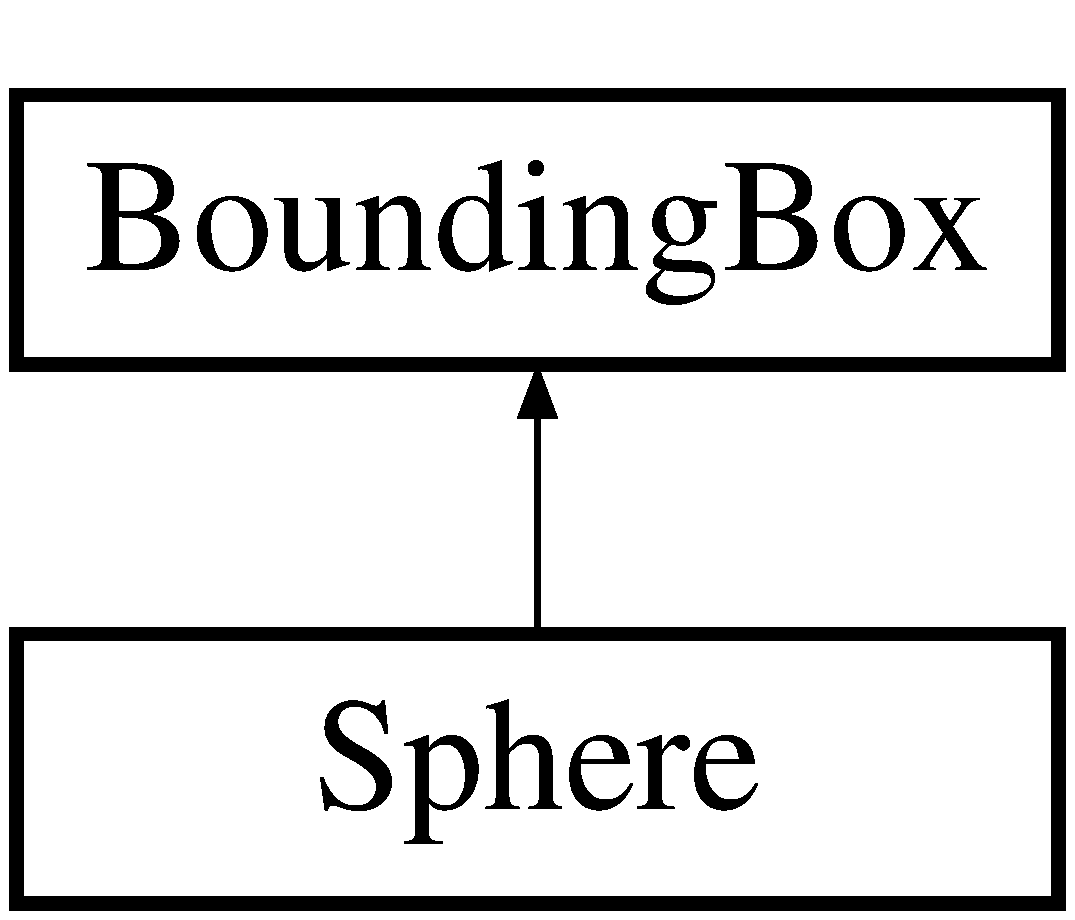
\includegraphics[height=2.000000cm]{class_sphere}
\end{center}
\end{figure}
\subsection*{Public Member Functions}
\begin{DoxyCompactItemize}
\item 
\hyperlink{class_sphere_a890a63ff583cb88e7ec4e840b4ef5eb9}{Sphere} ()
\item 
\hyperlink{class_sphere_a066dd77d24d95f7cb2e16880b3a5ae6e}{Sphere} (float \hyperlink{class_sphere_ae6f42f0da6679a2f0b4a22681ccccf38}{radius})
\item 
\hyperlink{class_sphere_a569c071e50a3e11f678630ee1a17737e}{$\sim$\-Sphere} ()
\end{DoxyCompactItemize}
\subsection*{Public Attributes}
\begin{DoxyCompactItemize}
\item 
float \hyperlink{class_sphere_ae6f42f0da6679a2f0b4a22681ccccf38}{radius}
\end{DoxyCompactItemize}
\subsection*{Additional Inherited Members}


\subsection{Detailed Description}


Definition at line 229 of file Comp\-Core.\-h.



\subsection{Constructor \& Destructor Documentation}
\hypertarget{class_sphere_a890a63ff583cb88e7ec4e840b4ef5eb9}{\index{Sphere@{Sphere}!Sphere@{Sphere}}
\index{Sphere@{Sphere}!Sphere@{Sphere}}
\subsubsection[{Sphere}]{\setlength{\rightskip}{0pt plus 5cm}Sphere\-::\-Sphere (
\begin{DoxyParamCaption}
{}
\end{DoxyParamCaption}
)}}\label{class_sphere_a890a63ff583cb88e7ec4e840b4ef5eb9}


Definition at line 238 of file Comp\-Core.\-cpp.

\hypertarget{class_sphere_a066dd77d24d95f7cb2e16880b3a5ae6e}{\index{Sphere@{Sphere}!Sphere@{Sphere}}
\index{Sphere@{Sphere}!Sphere@{Sphere}}
\subsubsection[{Sphere}]{\setlength{\rightskip}{0pt plus 5cm}Sphere\-::\-Sphere (
\begin{DoxyParamCaption}
\item[{float}]{radius}
\end{DoxyParamCaption}
)}}\label{class_sphere_a066dd77d24d95f7cb2e16880b3a5ae6e}


Definition at line 243 of file Comp\-Core.\-cpp.

\hypertarget{class_sphere_a569c071e50a3e11f678630ee1a17737e}{\index{Sphere@{Sphere}!$\sim$\-Sphere@{$\sim$\-Sphere}}
\index{$\sim$\-Sphere@{$\sim$\-Sphere}!Sphere@{Sphere}}
\subsubsection[{$\sim$\-Sphere}]{\setlength{\rightskip}{0pt plus 5cm}Sphere\-::$\sim$\-Sphere (
\begin{DoxyParamCaption}
{}
\end{DoxyParamCaption}
)}}\label{class_sphere_a569c071e50a3e11f678630ee1a17737e}


Definition at line 248 of file Comp\-Core.\-cpp.



\subsection{Member Data Documentation}
\hypertarget{class_sphere_ae6f42f0da6679a2f0b4a22681ccccf38}{\index{Sphere@{Sphere}!radius@{radius}}
\index{radius@{radius}!Sphere@{Sphere}}
\subsubsection[{radius}]{\setlength{\rightskip}{0pt plus 5cm}float Sphere\-::radius}}\label{class_sphere_ae6f42f0da6679a2f0b4a22681ccccf38}


Definition at line 231 of file Comp\-Core.\-h.



The documentation for this class was generated from the following files\-:\begin{DoxyCompactItemize}
\item 
\hyperlink{_comp_core_8h}{Comp\-Core.\-h}\item 
\hyperlink{_comp_core_8cpp}{Comp\-Core.\-cpp}\end{DoxyCompactItemize}

\hypertarget{class_static_obj}{\section{Static\-Obj Class Reference}
\label{class_static_obj}\index{Static\-Obj@{Static\-Obj}}
}


{\ttfamily \#include $<$static\-Obj.\-h$>$}

\subsection*{Public Member Functions}
\begin{DoxyCompactItemize}
\item 
\hyperlink{class_static_obj_adedc6727f2488cc926eb10ceaf7bce24}{Static\-Obj} (const char $\ast$obj\-File)
\item 
\hyperlink{class_static_obj_a0e9ad78e77930dd179a61892c101c7c7}{$\sim$\-Static\-Obj} ()
\item 
void \hyperlink{class_static_obj_a2bdd72e3c2edf70d8548f3a7ac86f91b}{draw\-All\-Objects} ()
\begin{DoxyCompactList}\small\item\em Deseneaza toate obiectele statice. \end{DoxyCompactList}\end{DoxyCompactItemize}
\subsection*{Static Public Member Functions}
\begin{DoxyCompactItemize}
\item 
static void \hyperlink{class_static_obj_a6216559c49acd38e5907f31477a1a766}{read\-Obj} (char $\ast$filename, \hyperlink{structobject}{object} \&comp)
\begin{DoxyCompactList}\small\item\em citeste in \end{DoxyCompactList}\item 
static void \hyperlink{class_static_obj_ab313f0fbec00b84e213d768fc48bec16}{load\-Texture} (char $\ast$filename, \hyperlink{structobject}{object} \&comp)
\item 
static void \hyperlink{class_static_obj_aff189588cac999afa0c5df1481d1b2d6}{draw\-Sky} ()
\begin{DoxyCompactList}\small\item\em Deseneaza sky-\/box-\/ul care este o semisfera, nu este desenat folosind metoda pentru obiecte normale deoarece locatia variaza neperiodic. \end{DoxyCompactList}\item 
static void \hyperlink{class_static_obj_a5eb942a526132f44ca7318bfcafbfd1c}{draw\-Object} (\hyperlink{structobject}{object} \&comp)
\begin{DoxyCompactList}\small\item\em Deseneaza obiectul static. \end{DoxyCompactList}\item 
static void \hyperlink{class_static_obj_ae7e5cc75f69f16475c1a5215fe3d1509}{set\-Object\-Id} (\hyperlink{structobject}{object} \&comp)
\begin{DoxyCompactList}\small\item\em Creeaza vertex buffer object si indices buffer object pe care ii incarca in memoria G\-P\-U, si seteaza id-\/urile din clasa object. \end{DoxyCompactList}\end{DoxyCompactItemize}
\subsection*{Public Attributes}
\begin{DoxyCompactItemize}
\item 
std\-::vector$<$ \hyperlink{structobject}{object} $>$ \hyperlink{class_static_obj_a926bfb30d4479a9fc6eb2fe3eeadbabc}{components}
\end{DoxyCompactItemize}


\subsection{Detailed Description}
obiectele statice din scena sau care se comporta periodic 

Definition at line 23 of file static\-Obj.\-h.



\subsection{Constructor \& Destructor Documentation}
\hypertarget{class_static_obj_adedc6727f2488cc926eb10ceaf7bce24}{\index{Static\-Obj@{Static\-Obj}!Static\-Obj@{Static\-Obj}}
\index{Static\-Obj@{Static\-Obj}!StaticObj@{Static\-Obj}}
\subsubsection[{Static\-Obj}]{\setlength{\rightskip}{0pt plus 5cm}Static\-Obj\-::\-Static\-Obj (
\begin{DoxyParamCaption}
\item[{const char $\ast$}]{obj\-File}
\end{DoxyParamCaption}
)\hspace{0.3cm}{\ttfamily [explicit]}}}\label{class_static_obj_adedc6727f2488cc926eb10ceaf7bce24}

\begin{DoxyParams}{Parameters}
{\em obj\-File} & este numele fisierului de configuare A se vedea formatul fisierelor \\
\hline
\end{DoxyParams}


Definition at line 10 of file static\-Obj.\-cpp.

\hypertarget{class_static_obj_a0e9ad78e77930dd179a61892c101c7c7}{\index{Static\-Obj@{Static\-Obj}!$\sim$\-Static\-Obj@{$\sim$\-Static\-Obj}}
\index{$\sim$\-Static\-Obj@{$\sim$\-Static\-Obj}!StaticObj@{Static\-Obj}}
\subsubsection[{$\sim$\-Static\-Obj}]{\setlength{\rightskip}{0pt plus 5cm}Static\-Obj\-::$\sim$\-Static\-Obj (
\begin{DoxyParamCaption}
{}
\end{DoxyParamCaption}
)}}\label{class_static_obj_a0e9ad78e77930dd179a61892c101c7c7}


Definition at line 83 of file static\-Obj.\-cpp.



\subsection{Member Function Documentation}
\hypertarget{class_static_obj_a2bdd72e3c2edf70d8548f3a7ac86f91b}{\index{Static\-Obj@{Static\-Obj}!draw\-All\-Objects@{draw\-All\-Objects}}
\index{draw\-All\-Objects@{draw\-All\-Objects}!StaticObj@{Static\-Obj}}
\subsubsection[{draw\-All\-Objects}]{\setlength{\rightskip}{0pt plus 5cm}void Static\-Obj\-::draw\-All\-Objects (
\begin{DoxyParamCaption}
{}
\end{DoxyParamCaption}
)}}\label{class_static_obj_a2bdd72e3c2edf70d8548f3a7ac86f91b}


Deseneaza toate obiectele statice. 



Definition at line 208 of file static\-Obj.\-cpp.

\hypertarget{class_static_obj_a5eb942a526132f44ca7318bfcafbfd1c}{\index{Static\-Obj@{Static\-Obj}!draw\-Object@{draw\-Object}}
\index{draw\-Object@{draw\-Object}!StaticObj@{Static\-Obj}}
\subsubsection[{draw\-Object}]{\setlength{\rightskip}{0pt plus 5cm}void Static\-Obj\-::draw\-Object (
\begin{DoxyParamCaption}
\item[{{\bf object} \&}]{comp}
\end{DoxyParamCaption}
)\hspace{0.3cm}{\ttfamily [static]}}}\label{class_static_obj_a5eb942a526132f44ca7318bfcafbfd1c}


Deseneaza obiectul static. 


\begin{DoxyParams}{Parameters}
{\em comp} & \\
\hline
\end{DoxyParams}


Definition at line 285 of file static\-Obj.\-cpp.

\hypertarget{class_static_obj_aff189588cac999afa0c5df1481d1b2d6}{\index{Static\-Obj@{Static\-Obj}!draw\-Sky@{draw\-Sky}}
\index{draw\-Sky@{draw\-Sky}!StaticObj@{Static\-Obj}}
\subsubsection[{draw\-Sky}]{\setlength{\rightskip}{0pt plus 5cm}void Static\-Obj\-::draw\-Sky (
\begin{DoxyParamCaption}
{}
\end{DoxyParamCaption}
)\hspace{0.3cm}{\ttfamily [static]}}}\label{class_static_obj_aff189588cac999afa0c5df1481d1b2d6}


Deseneaza sky-\/box-\/ul care este o semisfera, nu este desenat folosind metoda pentru obiecte normale deoarece locatia variaza neperiodic. 



Definition at line 197 of file static\-Obj.\-cpp.

\hypertarget{class_static_obj_ab313f0fbec00b84e213d768fc48bec16}{\index{Static\-Obj@{Static\-Obj}!load\-Texture@{load\-Texture}}
\index{load\-Texture@{load\-Texture}!StaticObj@{Static\-Obj}}
\subsubsection[{load\-Texture}]{\setlength{\rightskip}{0pt plus 5cm}void Static\-Obj\-::load\-Texture (
\begin{DoxyParamCaption}
\item[{char $\ast$}]{filename, }
\item[{{\bf object} \&}]{comp}
\end{DoxyParamCaption}
)\hspace{0.3cm}{\ttfamily [static]}}}\label{class_static_obj_ab313f0fbec00b84e213d768fc48bec16}

\begin{DoxyParams}{Parameters}
{\em incarca} & textura in format T\-G\-A 4\-B necompresata de la adresa \\
\hline
{\em filename} & in biectul \\
\hline
{\em comp} & \\
\hline
\end{DoxyParams}


Definition at line 168 of file static\-Obj.\-cpp.

\hypertarget{class_static_obj_a6216559c49acd38e5907f31477a1a766}{\index{Static\-Obj@{Static\-Obj}!read\-Obj@{read\-Obj}}
\index{read\-Obj@{read\-Obj}!StaticObj@{Static\-Obj}}
\subsubsection[{read\-Obj}]{\setlength{\rightskip}{0pt plus 5cm}void Static\-Obj\-::read\-Obj (
\begin{DoxyParamCaption}
\item[{char $\ast$}]{filename, }
\item[{{\bf object} \&}]{comp}
\end{DoxyParamCaption}
)\hspace{0.3cm}{\ttfamily [static]}}}\label{class_static_obj_a6216559c49acd38e5907f31477a1a766}


citeste in 


\begin{DoxyParams}{Parameters}
{\em comp,obiectul} & de tip.\-obj cde la adresa \\
\hline
{\em filename} & \\
\hline
\end{DoxyParams}


Definition at line 87 of file static\-Obj.\-cpp.

\hypertarget{class_static_obj_ae7e5cc75f69f16475c1a5215fe3d1509}{\index{Static\-Obj@{Static\-Obj}!set\-Object\-Id@{set\-Object\-Id}}
\index{set\-Object\-Id@{set\-Object\-Id}!StaticObj@{Static\-Obj}}
\subsubsection[{set\-Object\-Id}]{\setlength{\rightskip}{0pt plus 5cm}void Static\-Obj\-::set\-Object\-Id (
\begin{DoxyParamCaption}
\item[{{\bf object} \&}]{comp}
\end{DoxyParamCaption}
)\hspace{0.3cm}{\ttfamily [static]}}}\label{class_static_obj_ae7e5cc75f69f16475c1a5215fe3d1509}


Creeaza vertex buffer object si indices buffer object pe care ii incarca in memoria G\-P\-U, si seteaza id-\/urile din clasa object. 



Definition at line 121 of file static\-Obj.\-cpp.



\subsection{Member Data Documentation}
\hypertarget{class_static_obj_a926bfb30d4479a9fc6eb2fe3eeadbabc}{\index{Static\-Obj@{Static\-Obj}!components@{components}}
\index{components@{components}!StaticObj@{Static\-Obj}}
\subsubsection[{components}]{\setlength{\rightskip}{0pt plus 5cm}std\-::vector$<${\bf object}$>$ Static\-Obj\-::components}}\label{class_static_obj_a926bfb30d4479a9fc6eb2fe3eeadbabc}


Definition at line 25 of file static\-Obj.\-h.



The documentation for this class was generated from the following files\-:\begin{DoxyCompactItemize}
\item 
\hyperlink{static_obj_8h}{static\-Obj.\-h}\item 
\hyperlink{static_obj_8cpp}{static\-Obj.\-cpp}\end{DoxyCompactItemize}

\hypertarget{struct_targa_header}{\section{Targa\-Header Struct Reference}
\label{struct_targa_header}\index{Targa\-Header@{Targa\-Header}}
}


{\ttfamily \#include $<$T\-G\-A\-Image.\-h$>$}

\subsection*{Public Attributes}
\begin{DoxyCompactItemize}
\item 
unsigned char \hyperlink{struct_targa_header_a524d6939e514516a0ebd484f6aa6e19b}{id\-Length}
\item 
unsigned char \hyperlink{struct_targa_header_af972cd75dd815e9ca7d1b30d5ded3880}{color\-Map\-Type}
\item 
unsigned char \hyperlink{struct_targa_header_af1dbc0ea2e05d42678ff51c6cc43b630}{image\-Type\-Code}
\item 
unsigned char \hyperlink{struct_targa_header_a486c82f94722d32eb0c4c2c8344d9714}{color\-Map\-Spec} \mbox{[}5\mbox{]}
\item 
unsigned short \hyperlink{struct_targa_header_af1e612255d864f0c4c7f0689313b1408}{x\-Origin}
\item 
unsigned short \hyperlink{struct_targa_header_aaf344ab9c2e3d4c2146d478274f84724}{y\-Origin}
\item 
unsigned short \hyperlink{struct_targa_header_a3725c3553a93e16ba987c2b71e3c2b8b}{width}
\item 
unsigned short \hyperlink{struct_targa_header_a480252aac98d30159e726798679c9ee6}{height}
\item 
unsigned char \hyperlink{struct_targa_header_a808bc7fd8269ba401a755f54d973e803}{bpp}
\item 
unsigned char \hyperlink{struct_targa_header_ae575637b398fc5dab73ebe83bd28a217}{image\-Desc}
\end{DoxyCompactItemize}


\subsection{Detailed Description}
elementele unui format T\-G\-A 

Definition at line 8 of file T\-G\-A\-Image.\-h.



\subsection{Member Data Documentation}
\hypertarget{struct_targa_header_a808bc7fd8269ba401a755f54d973e803}{\index{Targa\-Header@{Targa\-Header}!bpp@{bpp}}
\index{bpp@{bpp}!TargaHeader@{Targa\-Header}}
\subsubsection[{bpp}]{\setlength{\rightskip}{0pt plus 5cm}unsigned char Targa\-Header\-::bpp}}\label{struct_targa_header_a808bc7fd8269ba401a755f54d973e803}


Definition at line 17 of file T\-G\-A\-Image.\-h.

\hypertarget{struct_targa_header_a486c82f94722d32eb0c4c2c8344d9714}{\index{Targa\-Header@{Targa\-Header}!color\-Map\-Spec@{color\-Map\-Spec}}
\index{color\-Map\-Spec@{color\-Map\-Spec}!TargaHeader@{Targa\-Header}}
\subsubsection[{color\-Map\-Spec}]{\setlength{\rightskip}{0pt plus 5cm}unsigned char Targa\-Header\-::color\-Map\-Spec\mbox{[}5\mbox{]}}}\label{struct_targa_header_a486c82f94722d32eb0c4c2c8344d9714}


Definition at line 12 of file T\-G\-A\-Image.\-h.

\hypertarget{struct_targa_header_af972cd75dd815e9ca7d1b30d5ded3880}{\index{Targa\-Header@{Targa\-Header}!color\-Map\-Type@{color\-Map\-Type}}
\index{color\-Map\-Type@{color\-Map\-Type}!TargaHeader@{Targa\-Header}}
\subsubsection[{color\-Map\-Type}]{\setlength{\rightskip}{0pt plus 5cm}unsigned char Targa\-Header\-::color\-Map\-Type}}\label{struct_targa_header_af972cd75dd815e9ca7d1b30d5ded3880}


Definition at line 10 of file T\-G\-A\-Image.\-h.

\hypertarget{struct_targa_header_a480252aac98d30159e726798679c9ee6}{\index{Targa\-Header@{Targa\-Header}!height@{height}}
\index{height@{height}!TargaHeader@{Targa\-Header}}
\subsubsection[{height}]{\setlength{\rightskip}{0pt plus 5cm}unsigned short Targa\-Header\-::height}}\label{struct_targa_header_a480252aac98d30159e726798679c9ee6}


Definition at line 16 of file T\-G\-A\-Image.\-h.

\hypertarget{struct_targa_header_a524d6939e514516a0ebd484f6aa6e19b}{\index{Targa\-Header@{Targa\-Header}!id\-Length@{id\-Length}}
\index{id\-Length@{id\-Length}!TargaHeader@{Targa\-Header}}
\subsubsection[{id\-Length}]{\setlength{\rightskip}{0pt plus 5cm}unsigned char Targa\-Header\-::id\-Length}}\label{struct_targa_header_a524d6939e514516a0ebd484f6aa6e19b}


Definition at line 9 of file T\-G\-A\-Image.\-h.

\hypertarget{struct_targa_header_ae575637b398fc5dab73ebe83bd28a217}{\index{Targa\-Header@{Targa\-Header}!image\-Desc@{image\-Desc}}
\index{image\-Desc@{image\-Desc}!TargaHeader@{Targa\-Header}}
\subsubsection[{image\-Desc}]{\setlength{\rightskip}{0pt plus 5cm}unsigned char Targa\-Header\-::image\-Desc}}\label{struct_targa_header_ae575637b398fc5dab73ebe83bd28a217}


Definition at line 18 of file T\-G\-A\-Image.\-h.

\hypertarget{struct_targa_header_af1dbc0ea2e05d42678ff51c6cc43b630}{\index{Targa\-Header@{Targa\-Header}!image\-Type\-Code@{image\-Type\-Code}}
\index{image\-Type\-Code@{image\-Type\-Code}!TargaHeader@{Targa\-Header}}
\subsubsection[{image\-Type\-Code}]{\setlength{\rightskip}{0pt plus 5cm}unsigned char Targa\-Header\-::image\-Type\-Code}}\label{struct_targa_header_af1dbc0ea2e05d42678ff51c6cc43b630}


Definition at line 11 of file T\-G\-A\-Image.\-h.

\hypertarget{struct_targa_header_a3725c3553a93e16ba987c2b71e3c2b8b}{\index{Targa\-Header@{Targa\-Header}!width@{width}}
\index{width@{width}!TargaHeader@{Targa\-Header}}
\subsubsection[{width}]{\setlength{\rightskip}{0pt plus 5cm}unsigned short Targa\-Header\-::width}}\label{struct_targa_header_a3725c3553a93e16ba987c2b71e3c2b8b}


Definition at line 15 of file T\-G\-A\-Image.\-h.

\hypertarget{struct_targa_header_af1e612255d864f0c4c7f0689313b1408}{\index{Targa\-Header@{Targa\-Header}!x\-Origin@{x\-Origin}}
\index{x\-Origin@{x\-Origin}!TargaHeader@{Targa\-Header}}
\subsubsection[{x\-Origin}]{\setlength{\rightskip}{0pt plus 5cm}unsigned short Targa\-Header\-::x\-Origin}}\label{struct_targa_header_af1e612255d864f0c4c7f0689313b1408}


Definition at line 13 of file T\-G\-A\-Image.\-h.

\hypertarget{struct_targa_header_aaf344ab9c2e3d4c2146d478274f84724}{\index{Targa\-Header@{Targa\-Header}!y\-Origin@{y\-Origin}}
\index{y\-Origin@{y\-Origin}!TargaHeader@{Targa\-Header}}
\subsubsection[{y\-Origin}]{\setlength{\rightskip}{0pt plus 5cm}unsigned short Targa\-Header\-::y\-Origin}}\label{struct_targa_header_aaf344ab9c2e3d4c2146d478274f84724}


Definition at line 14 of file T\-G\-A\-Image.\-h.



The documentation for this struct was generated from the following file\-:\begin{DoxyCompactItemize}
\item 
\hyperlink{_t_g_a_image_8h}{T\-G\-A\-Image.\-h}\end{DoxyCompactItemize}

\hypertarget{struct_texel_r_g_b}{\section{Texel\-R\-G\-B Struct Reference}
\label{struct_texel_r_g_b}\index{Texel\-R\-G\-B@{Texel\-R\-G\-B}}
}


{\ttfamily \#include $<$Comp\-Core.\-h$>$}

\subsection*{Public Attributes}
\begin{DoxyCompactItemize}
\item 
unsigned char \hyperlink{struct_texel_r_g_b_ad62f973f1db93f3c02e5288ec0fb32c8}{r}
\item 
unsigned char \hyperlink{struct_texel_r_g_b_a9de470616b6b5ef114bf3806c12142dc}{g}
\item 
unsigned char \hyperlink{struct_texel_r_g_b_ac524adc8d2190f021f42f24aea7dc1a2}{b}
\end{DoxyCompactItemize}


\subsection{Detailed Description}
exclusiv pentru citirea imaginilor T\-G\-A, poate fi utila in alte situatii 

Definition at line 174 of file Comp\-Core.\-h.



\subsection{Member Data Documentation}
\hypertarget{struct_texel_r_g_b_ac524adc8d2190f021f42f24aea7dc1a2}{\index{Texel\-R\-G\-B@{Texel\-R\-G\-B}!b@{b}}
\index{b@{b}!TexelRGB@{Texel\-R\-G\-B}}
\subsubsection[{b}]{\setlength{\rightskip}{0pt plus 5cm}unsigned char Texel\-R\-G\-B\-::b}}\label{struct_texel_r_g_b_ac524adc8d2190f021f42f24aea7dc1a2}


Definition at line 175 of file Comp\-Core.\-h.

\hypertarget{struct_texel_r_g_b_a9de470616b6b5ef114bf3806c12142dc}{\index{Texel\-R\-G\-B@{Texel\-R\-G\-B}!g@{g}}
\index{g@{g}!TexelRGB@{Texel\-R\-G\-B}}
\subsubsection[{g}]{\setlength{\rightskip}{0pt plus 5cm}unsigned char Texel\-R\-G\-B\-::g}}\label{struct_texel_r_g_b_a9de470616b6b5ef114bf3806c12142dc}


Definition at line 175 of file Comp\-Core.\-h.

\hypertarget{struct_texel_r_g_b_ad62f973f1db93f3c02e5288ec0fb32c8}{\index{Texel\-R\-G\-B@{Texel\-R\-G\-B}!r@{r}}
\index{r@{r}!TexelRGB@{Texel\-R\-G\-B}}
\subsubsection[{r}]{\setlength{\rightskip}{0pt plus 5cm}unsigned char Texel\-R\-G\-B\-::r}}\label{struct_texel_r_g_b_ad62f973f1db93f3c02e5288ec0fb32c8}


Definition at line 175 of file Comp\-Core.\-h.



The documentation for this struct was generated from the following file\-:\begin{DoxyCompactItemize}
\item 
\hyperlink{_comp_core_8h}{Comp\-Core.\-h}\end{DoxyCompactItemize}

\hypertarget{struct_texel_r_g_b_a}{\section{Texel\-R\-G\-B\-A Struct Reference}
\label{struct_texel_r_g_b_a}\index{Texel\-R\-G\-B\-A@{Texel\-R\-G\-B\-A}}
}


{\ttfamily \#include $<$Comp\-Core.\-h$>$}

\subsection*{Public Attributes}
\begin{DoxyCompactItemize}
\item 
unsigned char \hyperlink{struct_texel_r_g_b_a_a35804d005988bece75db0928273cd74d}{r}
\item 
unsigned char \hyperlink{struct_texel_r_g_b_a_a997ab15a88f5114bed505733605a3862}{g}
\item 
unsigned char \hyperlink{struct_texel_r_g_b_a_adac5a2af26ec9605db3f6fa59a1ca7d3}{b}
\item 
unsigned char \hyperlink{struct_texel_r_g_b_a_a3bffb7b8858479123e0c1e3abd53b541}{a}
\end{DoxyCompactItemize}


\subsection{Detailed Description}
exclusiv pentru citirea imaginilor T\-G\-A, poate fi utila in alte situatii 

Definition at line 166 of file Comp\-Core.\-h.



\subsection{Member Data Documentation}
\hypertarget{struct_texel_r_g_b_a_a3bffb7b8858479123e0c1e3abd53b541}{\index{Texel\-R\-G\-B\-A@{Texel\-R\-G\-B\-A}!a@{a}}
\index{a@{a}!TexelRGBA@{Texel\-R\-G\-B\-A}}
\subsubsection[{a}]{\setlength{\rightskip}{0pt plus 5cm}unsigned char Texel\-R\-G\-B\-A\-::a}}\label{struct_texel_r_g_b_a_a3bffb7b8858479123e0c1e3abd53b541}


Definition at line 167 of file Comp\-Core.\-h.

\hypertarget{struct_texel_r_g_b_a_adac5a2af26ec9605db3f6fa59a1ca7d3}{\index{Texel\-R\-G\-B\-A@{Texel\-R\-G\-B\-A}!b@{b}}
\index{b@{b}!TexelRGBA@{Texel\-R\-G\-B\-A}}
\subsubsection[{b}]{\setlength{\rightskip}{0pt plus 5cm}unsigned char Texel\-R\-G\-B\-A\-::b}}\label{struct_texel_r_g_b_a_adac5a2af26ec9605db3f6fa59a1ca7d3}


Definition at line 167 of file Comp\-Core.\-h.

\hypertarget{struct_texel_r_g_b_a_a997ab15a88f5114bed505733605a3862}{\index{Texel\-R\-G\-B\-A@{Texel\-R\-G\-B\-A}!g@{g}}
\index{g@{g}!TexelRGBA@{Texel\-R\-G\-B\-A}}
\subsubsection[{g}]{\setlength{\rightskip}{0pt plus 5cm}unsigned char Texel\-R\-G\-B\-A\-::g}}\label{struct_texel_r_g_b_a_a997ab15a88f5114bed505733605a3862}


Definition at line 167 of file Comp\-Core.\-h.

\hypertarget{struct_texel_r_g_b_a_a35804d005988bece75db0928273cd74d}{\index{Texel\-R\-G\-B\-A@{Texel\-R\-G\-B\-A}!r@{r}}
\index{r@{r}!TexelRGBA@{Texel\-R\-G\-B\-A}}
\subsubsection[{r}]{\setlength{\rightskip}{0pt plus 5cm}unsigned char Texel\-R\-G\-B\-A\-::r}}\label{struct_texel_r_g_b_a_a35804d005988bece75db0928273cd74d}


Definition at line 167 of file Comp\-Core.\-h.



The documentation for this struct was generated from the following file\-:\begin{DoxyCompactItemize}
\item 
\hyperlink{_comp_core_8h}{Comp\-Core.\-h}\end{DoxyCompactItemize}

\hypertarget{class_t_g_a_image}{\section{T\-G\-A\-Image Class Reference}
\label{class_t_g_a_image}\index{T\-G\-A\-Image@{T\-G\-A\-Image}}
}


{\ttfamily \#include $<$T\-G\-A\-Image.\-h$>$}

\subsection*{Public Member Functions}
\begin{DoxyCompactItemize}
\item 
\hyperlink{class_t_g_a_image_a790b74801c879879bebe9e2ec2e04529}{T\-G\-A\-Image} (char $\ast$filename)
\item 
\hyperlink{class_t_g_a_image_a3b3d841039c8a6da816603f6f2933420}{$\sim$\-T\-G\-A\-Image} ()
\item 
virtual bool \hyperlink{class_t_g_a_image_ac68656afca46d4aedafaf55f8dff5ba6}{load\-File} (char $\ast$filename)
\item 
void \hyperlink{class_t_g_a_image_a39f001590a444a19145c388ac75139a0}{B\-G\-Rto\-R\-G\-B} ()
\begin{DoxyCompactList}\small\item\em Modifica octetii pentru a fi incarcati in memoria textura. \end{DoxyCompactList}\end{DoxyCompactItemize}
\subsection*{Public Attributes}
\begin{DoxyCompactItemize}
\item 
unsigned char $\ast$ \hyperlink{class_t_g_a_image_afd06806bae721d61ae49a600ef26e6d1}{data}
\item 
unsigned int \hyperlink{class_t_g_a_image_a8a7bef4441a3cd17e237bee43e654b5a}{width}
\item 
unsigned int \hyperlink{class_t_g_a_image_a1c4a71ac195496eeaf7ed6d3e9dfe0ac}{height}
\end{DoxyCompactItemize}


\subsection{Detailed Description}
care citeste o imagine T\-G\-A si o incarca in memoria G\-P\-U-\/ului 

Definition at line 26 of file T\-G\-A\-Image.\-h.



\subsection{Constructor \& Destructor Documentation}
\hypertarget{class_t_g_a_image_a790b74801c879879bebe9e2ec2e04529}{\index{T\-G\-A\-Image@{T\-G\-A\-Image}!T\-G\-A\-Image@{T\-G\-A\-Image}}
\index{T\-G\-A\-Image@{T\-G\-A\-Image}!TGAImage@{T\-G\-A\-Image}}
\subsubsection[{T\-G\-A\-Image}]{\setlength{\rightskip}{0pt plus 5cm}T\-G\-A\-Image\-::\-T\-G\-A\-Image (
\begin{DoxyParamCaption}
\item[{char $\ast$}]{filename}
\end{DoxyParamCaption}
)\hspace{0.3cm}{\ttfamily [explicit]}}}\label{class_t_g_a_image_a790b74801c879879bebe9e2ec2e04529}


Definition at line 3 of file T\-G\-A\-Image.\-cpp.

\hypertarget{class_t_g_a_image_a3b3d841039c8a6da816603f6f2933420}{\index{T\-G\-A\-Image@{T\-G\-A\-Image}!$\sim$\-T\-G\-A\-Image@{$\sim$\-T\-G\-A\-Image}}
\index{$\sim$\-T\-G\-A\-Image@{$\sim$\-T\-G\-A\-Image}!TGAImage@{T\-G\-A\-Image}}
\subsubsection[{$\sim$\-T\-G\-A\-Image}]{\setlength{\rightskip}{0pt plus 5cm}T\-G\-A\-Image\-::$\sim$\-T\-G\-A\-Image (
\begin{DoxyParamCaption}
{}
\end{DoxyParamCaption}
)}}\label{class_t_g_a_image_a3b3d841039c8a6da816603f6f2933420}
\begin{DoxyAttention}{Attention}
Do not delete 
\end{DoxyAttention}

\begin{DoxyParams}{Parameters}
{\em data} & \\
\hline
\end{DoxyParams}


Definition at line 12 of file T\-G\-A\-Image.\-cpp.



\subsection{Member Function Documentation}
\hypertarget{class_t_g_a_image_a39f001590a444a19145c388ac75139a0}{\index{T\-G\-A\-Image@{T\-G\-A\-Image}!B\-G\-Rto\-R\-G\-B@{B\-G\-Rto\-R\-G\-B}}
\index{B\-G\-Rto\-R\-G\-B@{B\-G\-Rto\-R\-G\-B}!TGAImage@{T\-G\-A\-Image}}
\subsubsection[{B\-G\-Rto\-R\-G\-B}]{\setlength{\rightskip}{0pt plus 5cm}void T\-G\-A\-Image\-::\-B\-G\-Rto\-R\-G\-B (
\begin{DoxyParamCaption}
{}
\end{DoxyParamCaption}
)}}\label{class_t_g_a_image_a39f001590a444a19145c388ac75139a0}


Modifica octetii pentru a fi incarcati in memoria textura. 



Definition at line 32 of file T\-G\-A\-Image.\-cpp.

\hypertarget{class_t_g_a_image_ac68656afca46d4aedafaf55f8dff5ba6}{\index{T\-G\-A\-Image@{T\-G\-A\-Image}!load\-File@{load\-File}}
\index{load\-File@{load\-File}!TGAImage@{T\-G\-A\-Image}}
\subsubsection[{load\-File}]{\setlength{\rightskip}{0pt plus 5cm}bool T\-G\-A\-Image\-::load\-File (
\begin{DoxyParamCaption}
\item[{char $\ast$}]{filename}
\end{DoxyParamCaption}
)\hspace{0.3cm}{\ttfamily [virtual]}}}\label{class_t_g_a_image_ac68656afca46d4aedafaf55f8dff5ba6}


Definition at line 16 of file T\-G\-A\-Image.\-cpp.



\subsection{Member Data Documentation}
\hypertarget{class_t_g_a_image_afd06806bae721d61ae49a600ef26e6d1}{\index{T\-G\-A\-Image@{T\-G\-A\-Image}!data@{data}}
\index{data@{data}!TGAImage@{T\-G\-A\-Image}}
\subsubsection[{data}]{\setlength{\rightskip}{0pt plus 5cm}unsigned char$\ast$ T\-G\-A\-Image\-::data}}\label{class_t_g_a_image_afd06806bae721d61ae49a600ef26e6d1}


Definition at line 29 of file T\-G\-A\-Image.\-h.

\hypertarget{class_t_g_a_image_a1c4a71ac195496eeaf7ed6d3e9dfe0ac}{\index{T\-G\-A\-Image@{T\-G\-A\-Image}!height@{height}}
\index{height@{height}!TGAImage@{T\-G\-A\-Image}}
\subsubsection[{height}]{\setlength{\rightskip}{0pt plus 5cm}unsigned int T\-G\-A\-Image\-::height}}\label{class_t_g_a_image_a1c4a71ac195496eeaf7ed6d3e9dfe0ac}


Definition at line 30 of file T\-G\-A\-Image.\-h.

\hypertarget{class_t_g_a_image_a8a7bef4441a3cd17e237bee43e654b5a}{\index{T\-G\-A\-Image@{T\-G\-A\-Image}!width@{width}}
\index{width@{width}!TGAImage@{T\-G\-A\-Image}}
\subsubsection[{width}]{\setlength{\rightskip}{0pt plus 5cm}unsigned int T\-G\-A\-Image\-::width}}\label{class_t_g_a_image_a8a7bef4441a3cd17e237bee43e654b5a}


Definition at line 30 of file T\-G\-A\-Image.\-h.



The documentation for this class was generated from the following files\-:\begin{DoxyCompactItemize}
\item 
\hyperlink{_t_g_a_image_8h}{T\-G\-A\-Image.\-h}\item 
\hyperlink{_t_g_a_image_8cpp}{T\-G\-A\-Image.\-cpp}\end{DoxyCompactItemize}

\hypertarget{struct_vector3}{\section{Vector3 Struct Reference}
\label{struct_vector3}\index{Vector3@{Vector3}}
}


{\ttfamily \#include $<$Comp\-Core.\-h$>$}

\subsection*{Public Member Functions}
\begin{DoxyCompactItemize}
\item 
\hyperlink{struct_vector3_ad53e22b52babdb90d423601f72467590}{Vector3} (float \hyperlink{struct_vector3_a7e2d3237b29a2f29d7b3d8b2934e35f2}{x}, float \hyperlink{struct_vector3_a86eb35a9fa2d5a49e7fad66a35fa9c13}{y}, float \hyperlink{struct_vector3_aa8c9461eb24bd2c364258078811a3e9d}{z})
\item 
\hyperlink{struct_vector3_a0f49191f7e001e7f7ae1cb49522118b4}{Vector3} ()
\item 
\hyperlink{struct_vector3_a5545e13e2e2861ece8f14b12a6a8101f}{$\sim$\-Vector3} ()
\item 
\hyperlink{struct_vector3}{Vector3} \hyperlink{struct_vector3_a6c1adee4e0d030153b6fd610897809c9}{operator+} (\hyperlink{struct_vector3}{Vector3} \&\hyperlink{struct_vector3_a7e2d3237b29a2f29d7b3d8b2934e35f2}{x})
\item 
\hyperlink{struct_vector3}{Vector3} \hyperlink{struct_vector3_a7ee2ab8be82ace8b8fca9e8dbb9d57af}{operator-\/} (\hyperlink{struct_vector3}{Vector3} \&\hyperlink{struct_vector3_a7e2d3237b29a2f29d7b3d8b2934e35f2}{x})
\item 
\hyperlink{struct_vector3}{Vector3} \hyperlink{struct_vector3_af70aac6ee8f570fcf6354288afcbba34}{operator/} (float \&m)
\begin{DoxyCompactList}\small\item\em Imparte fiecare element al vetorului la. \end{DoxyCompactList}\item 
\hyperlink{struct_vector3}{Vector3} \hyperlink{struct_vector3_a6e87944da5592f2649163d573873d758}{operator$\ast$} (float \&m)
\begin{DoxyCompactList}\small\item\em multiplica fiecare element al vectorului cu m \end{DoxyCompactList}\item 
float \hyperlink{struct_vector3_ac99f99d41cfbc35d7be65e0a7469ff79}{get\-Dist} (\hyperlink{struct_vector3}{Vector3} \&a)
\begin{DoxyCompactList}\small\item\em Afla distanta intre vectorul implicit si. \end{DoxyCompactList}\item 
virtual bool \hyperlink{struct_vector3_a065da1e1e6164259fc296a197aa4ea1e}{is\-Valid} ()
\begin{DoxyCompactList}\small\item\em Am convenit ca vectorul cu primul element -\/1 sa fie invalid metoda returneaza true daca elementul e valid false altfel. \end{DoxyCompactList}\item 
bool \hyperlink{struct_vector3_aecd46e467c12a408b98885faaa453c29}{is\-Inside} (\hyperlink{struct_vector3}{Vector3} \&a, \hyperlink{struct_vector3}{Vector3} \&b)
\begin{DoxyCompactList}\small\item\em Spne daca toate coordonatele vectorului curent sunt intre coordonatele celor 2 vectori. \end{DoxyCompactList}\item 
void \hyperlink{struct_vector3_aa2d4b629b2d1260a49a88bd98c48934a}{print} ()
\begin{DoxyCompactList}\small\item\em utilizata pentru Debugging, afiseaza coordonatele punctului curent. \end{DoxyCompactList}\end{DoxyCompactItemize}
\subsection*{Static Public Member Functions}
\begin{DoxyCompactItemize}
\item 
static void \hyperlink{struct_vector3_a19c258342bd0c27ddcd7e079d6d38b5f}{translate} (\hyperlink{struct_vector3}{Vector3} point)
\begin{DoxyCompactList}\small\item\em apeleaza functia gl\-Translatef cu parametrii vectorului {\bfseries point} \end{DoxyCompactList}\item 
static void \hyperlink{struct_vector3_a55239686f46937c64fec068f52a4d5b6}{rotate} (\hyperlink{struct_vector3}{Vector3} point, float angle)
\begin{DoxyCompactList}\small\item\em Apeleaza gl\-Rotatef cu quaternion-\/ul. \end{DoxyCompactList}\item 
static void \hyperlink{struct_vector3_a31279b5d53f5cf4f36f8a02ba826844b}{scale} (\hyperlink{struct_vector3}{Vector3} point)
\begin{DoxyCompactList}\small\item\em apeleaza functia gl\-Scalef cu parametrii \end{DoxyCompactList}\item 
static void \hyperlink{struct_vector3_a44b36db62c048090ee7b7eef7ce4ba3e}{translate\-Back} (\hyperlink{struct_vector3}{Vector3} point)
\begin{DoxyCompactList}\small\item\em \hyperlink{struct_face}{Face} miscare de translatie inversa pentru. \end{DoxyCompactList}\item 
static void \hyperlink{struct_vector3_a7fcc44e050a023b53c0745e6d7068019}{rotate\-Back} (\hyperlink{struct_vector3}{Vector3} point, float angle)
\begin{DoxyCompactList}\small\item\em \hyperlink{struct_face}{Face} rotatia inversa pentru quaternionul. \end{DoxyCompactList}\item 
static void \hyperlink{struct_vector3_a5a586e78bef39b3f2d22e30883aab5cb}{scale\-Back} (\hyperlink{struct_vector3}{Vector3} point)
\begin{DoxyCompactList}\small\item\em \hyperlink{struct_face}{Face} scalarea inversa pentru. \end{DoxyCompactList}\item 
static float \hyperlink{struct_vector3_a8b6eff7231a5595aafe938e1362de1ff}{get\-Dist} (\hyperlink{struct_vector3}{Vector3} \&a, \hyperlink{struct_vector3}{Vector3} \&b)
\begin{DoxyCompactList}\small\item\em calculeaza distanta intre 2 puncte in spatiu \end{DoxyCompactList}\item 
static \hyperlink{struct_vector3}{Vector3} \hyperlink{struct_vector3_a5dffe84d05c294364300dfd5a6ac6eee}{invalid\-Point} ()
\begin{DoxyCompactList}\small\item\em Returneaza vectorul invalid conform \char`\"{}intelegerii\char`\"{}. \end{DoxyCompactList}\end{DoxyCompactItemize}
\subsection*{Public Attributes}
\begin{DoxyCompactItemize}
\item 
float \hyperlink{struct_vector3_a7e2d3237b29a2f29d7b3d8b2934e35f2}{x}
\item 
float \hyperlink{struct_vector3_a86eb35a9fa2d5a49e7fad66a35fa9c13}{y}
\item 
float \hyperlink{struct_vector3_aa8c9461eb24bd2c364258078811a3e9d}{z}
\end{DoxyCompactItemize}


\subsection{Detailed Description}
care reprezinta un punct in spatiul 3d 

Definition at line 20 of file Comp\-Core.\-h.



\subsection{Constructor \& Destructor Documentation}
\hypertarget{struct_vector3_ad53e22b52babdb90d423601f72467590}{\index{Vector3@{Vector3}!Vector3@{Vector3}}
\index{Vector3@{Vector3}!Vector3@{Vector3}}
\subsubsection[{Vector3}]{\setlength{\rightskip}{0pt plus 5cm}Vector3\-::\-Vector3 (
\begin{DoxyParamCaption}
\item[{float}]{x, }
\item[{float}]{y, }
\item[{float}]{z}
\end{DoxyParamCaption}
)}}\label{struct_vector3_ad53e22b52babdb90d423601f72467590}


Definition at line 3 of file Comp\-Core.\-cpp.

\hypertarget{struct_vector3_a0f49191f7e001e7f7ae1cb49522118b4}{\index{Vector3@{Vector3}!Vector3@{Vector3}}
\index{Vector3@{Vector3}!Vector3@{Vector3}}
\subsubsection[{Vector3}]{\setlength{\rightskip}{0pt plus 5cm}Vector3\-::\-Vector3 (
\begin{DoxyParamCaption}
{}
\end{DoxyParamCaption}
)}}\label{struct_vector3_a0f49191f7e001e7f7ae1cb49522118b4}


Definition at line 10 of file Comp\-Core.\-cpp.

\hypertarget{struct_vector3_a5545e13e2e2861ece8f14b12a6a8101f}{\index{Vector3@{Vector3}!$\sim$\-Vector3@{$\sim$\-Vector3}}
\index{$\sim$\-Vector3@{$\sim$\-Vector3}!Vector3@{Vector3}}
\subsubsection[{$\sim$\-Vector3}]{\setlength{\rightskip}{0pt plus 5cm}Vector3\-::$\sim$\-Vector3 (
\begin{DoxyParamCaption}
{}
\end{DoxyParamCaption}
)}}\label{struct_vector3_a5545e13e2e2861ece8f14b12a6a8101f}


Definition at line 17 of file Comp\-Core.\-cpp.



\subsection{Member Function Documentation}
\hypertarget{struct_vector3_ac99f99d41cfbc35d7be65e0a7469ff79}{\index{Vector3@{Vector3}!get\-Dist@{get\-Dist}}
\index{get\-Dist@{get\-Dist}!Vector3@{Vector3}}
\subsubsection[{get\-Dist}]{\setlength{\rightskip}{0pt plus 5cm}float Vector3\-::get\-Dist (
\begin{DoxyParamCaption}
\item[{{\bf Vector3} \&}]{a}
\end{DoxyParamCaption}
)}}\label{struct_vector3_ac99f99d41cfbc35d7be65e0a7469ff79}


Afla distanta intre vectorul implicit si. 


\begin{DoxyParams}{Parameters}
{\em a} & \\
\hline
\end{DoxyParams}


Definition at line 86 of file Comp\-Core.\-cpp.

\hypertarget{struct_vector3_a8b6eff7231a5595aafe938e1362de1ff}{\index{Vector3@{Vector3}!get\-Dist@{get\-Dist}}
\index{get\-Dist@{get\-Dist}!Vector3@{Vector3}}
\subsubsection[{get\-Dist}]{\setlength{\rightskip}{0pt plus 5cm}float Vector3\-::get\-Dist (
\begin{DoxyParamCaption}
\item[{{\bf Vector3} \&}]{a, }
\item[{{\bf Vector3} \&}]{b}
\end{DoxyParamCaption}
)\hspace{0.3cm}{\ttfamily [static]}}}\label{struct_vector3_a8b6eff7231a5595aafe938e1362de1ff}


calculeaza distanta intre 2 puncte in spatiu 



Definition at line 91 of file Comp\-Core.\-cpp.

\hypertarget{struct_vector3_a5dffe84d05c294364300dfd5a6ac6eee}{\index{Vector3@{Vector3}!invalid\-Point@{invalid\-Point}}
\index{invalid\-Point@{invalid\-Point}!Vector3@{Vector3}}
\subsubsection[{invalid\-Point}]{\setlength{\rightskip}{0pt plus 5cm}{\bf Vector3} Vector3\-::invalid\-Point (
\begin{DoxyParamCaption}
{}
\end{DoxyParamCaption}
)\hspace{0.3cm}{\ttfamily [static]}}}\label{struct_vector3_a5dffe84d05c294364300dfd5a6ac6eee}


Returneaza vectorul invalid conform \char`\"{}intelegerii\char`\"{}. 

\begin{DoxyAttention}{Attention}
Trebuie avut grija la intervalul vectorilor valizi sa nu se suprapuna peste vectorul invalid 
\end{DoxyAttention}


Definition at line 96 of file Comp\-Core.\-cpp.

\hypertarget{struct_vector3_aecd46e467c12a408b98885faaa453c29}{\index{Vector3@{Vector3}!is\-Inside@{is\-Inside}}
\index{is\-Inside@{is\-Inside}!Vector3@{Vector3}}
\subsubsection[{is\-Inside}]{\setlength{\rightskip}{0pt plus 5cm}bool Vector3\-::is\-Inside (
\begin{DoxyParamCaption}
\item[{{\bf Vector3} \&}]{a, }
\item[{{\bf Vector3} \&}]{b}
\end{DoxyParamCaption}
)}}\label{struct_vector3_aecd46e467c12a408b98885faaa453c29}


Spne daca toate coordonatele vectorului curent sunt intre coordonatele celor 2 vectori. 



Definition at line 105 of file Comp\-Core.\-cpp.

\hypertarget{struct_vector3_a065da1e1e6164259fc296a197aa4ea1e}{\index{Vector3@{Vector3}!is\-Valid@{is\-Valid}}
\index{is\-Valid@{is\-Valid}!Vector3@{Vector3}}
\subsubsection[{is\-Valid}]{\setlength{\rightskip}{0pt plus 5cm}bool Vector3\-::is\-Valid (
\begin{DoxyParamCaption}
{}
\end{DoxyParamCaption}
)\hspace{0.3cm}{\ttfamily [virtual]}}}\label{struct_vector3_a065da1e1e6164259fc296a197aa4ea1e}


Am convenit ca vectorul cu primul element -\/1 sa fie invalid metoda returneaza true daca elementul e valid false altfel. 



Definition at line 116 of file Comp\-Core.\-cpp.

\hypertarget{struct_vector3_a6e87944da5592f2649163d573873d758}{\index{Vector3@{Vector3}!operator$\ast$@{operator$\ast$}}
\index{operator$\ast$@{operator$\ast$}!Vector3@{Vector3}}
\subsubsection[{operator$\ast$}]{\setlength{\rightskip}{0pt plus 5cm}{\bf Vector3} Vector3\-::operator$\ast$ (
\begin{DoxyParamCaption}
\item[{float \&}]{m}
\end{DoxyParamCaption}
)}}\label{struct_vector3_a6e87944da5592f2649163d573873d758}


multiplica fiecare element al vectorului cu m 



Definition at line 48 of file Comp\-Core.\-cpp.

\hypertarget{struct_vector3_a6c1adee4e0d030153b6fd610897809c9}{\index{Vector3@{Vector3}!operator+@{operator+}}
\index{operator+@{operator+}!Vector3@{Vector3}}
\subsubsection[{operator+}]{\setlength{\rightskip}{0pt plus 5cm}{\bf Vector3} Vector3\-::operator+ (
\begin{DoxyParamCaption}
\item[{{\bf Vector3} \&}]{x}
\end{DoxyParamCaption}
)}}\label{struct_vector3_a6c1adee4e0d030153b6fd610897809c9}
\begin{DoxyReturn}{Returns}
Va insuma elementele vectorilor. (a1, b1, c1) + (a2, b2, c2) = (a1+a2, b1+b2, c1+c2) 
\end{DoxyReturn}


Definition at line 21 of file Comp\-Core.\-cpp.

\hypertarget{struct_vector3_a7ee2ab8be82ace8b8fca9e8dbb9d57af}{\index{Vector3@{Vector3}!operator-\/@{operator-\/}}
\index{operator-\/@{operator-\/}!Vector3@{Vector3}}
\subsubsection[{operator-\/}]{\setlength{\rightskip}{0pt plus 5cm}{\bf Vector3} Vector3\-::operator-\/ (
\begin{DoxyParamCaption}
\item[{{\bf Vector3} \&}]{x}
\end{DoxyParamCaption}
)}}\label{struct_vector3_a7ee2ab8be82ace8b8fca9e8dbb9d57af}
\begin{DoxyReturn}{Returns}
The answer will be the difference of the two vectors (a1, b1, c1) -\/ (a2, b2, c2) = (a1-\/a2, b1-\/b2, c1-\/c2) 
\end{DoxyReturn}


Definition at line 30 of file Comp\-Core.\-cpp.

\hypertarget{struct_vector3_af70aac6ee8f570fcf6354288afcbba34}{\index{Vector3@{Vector3}!operator/@{operator/}}
\index{operator/@{operator/}!Vector3@{Vector3}}
\subsubsection[{operator/}]{\setlength{\rightskip}{0pt plus 5cm}{\bf Vector3} Vector3\-::operator/ (
\begin{DoxyParamCaption}
\item[{float \&}]{m}
\end{DoxyParamCaption}
)}}\label{struct_vector3_af70aac6ee8f570fcf6354288afcbba34}


Imparte fiecare element al vetorului la. 


\begin{DoxyParams}{Parameters}
{\em m} & \\
\hline
\end{DoxyParams}


Definition at line 39 of file Comp\-Core.\-cpp.

\hypertarget{struct_vector3_aa2d4b629b2d1260a49a88bd98c48934a}{\index{Vector3@{Vector3}!print@{print}}
\index{print@{print}!Vector3@{Vector3}}
\subsubsection[{print}]{\setlength{\rightskip}{0pt plus 5cm}void Vector3\-::print (
\begin{DoxyParamCaption}
{}
\end{DoxyParamCaption}
)}}\label{struct_vector3_aa2d4b629b2d1260a49a88bd98c48934a}


utilizata pentru Debugging, afiseaza coordonatele punctului curent. 

\begin{DoxyAttention}{Attention}
Desenarea pe ecran nu este testata 
\end{DoxyAttention}


Definition at line 123 of file Comp\-Core.\-cpp.

\hypertarget{struct_vector3_a55239686f46937c64fec068f52a4d5b6}{\index{Vector3@{Vector3}!rotate@{rotate}}
\index{rotate@{rotate}!Vector3@{Vector3}}
\subsubsection[{rotate}]{\setlength{\rightskip}{0pt plus 5cm}void Vector3\-::rotate (
\begin{DoxyParamCaption}
\item[{{\bf Vector3}}]{point, }
\item[{float}]{angle}
\end{DoxyParamCaption}
)\hspace{0.3cm}{\ttfamily [static]}}}\label{struct_vector3_a55239686f46937c64fec068f52a4d5b6}


Apeleaza gl\-Rotatef cu quaternion-\/ul. 


\begin{DoxyParams}{Parameters}
{\em point} & si \\
\hline
{\em angle} & \\
\hline
\end{DoxyParams}


Definition at line 61 of file Comp\-Core.\-cpp.

\hypertarget{struct_vector3_a7fcc44e050a023b53c0745e6d7068019}{\index{Vector3@{Vector3}!rotate\-Back@{rotate\-Back}}
\index{rotate\-Back@{rotate\-Back}!Vector3@{Vector3}}
\subsubsection[{rotate\-Back}]{\setlength{\rightskip}{0pt plus 5cm}void Vector3\-::rotate\-Back (
\begin{DoxyParamCaption}
\item[{{\bf Vector3}}]{point, }
\item[{float}]{angle}
\end{DoxyParamCaption}
)\hspace{0.3cm}{\ttfamily [static]}}}\label{struct_vector3_a7fcc44e050a023b53c0745e6d7068019}


\hyperlink{struct_face}{Face} rotatia inversa pentru quaternionul. 


\begin{DoxyParams}{Parameters}
{\em point} & si \\
\hline
{\em angle} & \\
\hline
\end{DoxyParams}


Definition at line 76 of file Comp\-Core.\-cpp.

\hypertarget{struct_vector3_a31279b5d53f5cf4f36f8a02ba826844b}{\index{Vector3@{Vector3}!scale@{scale}}
\index{scale@{scale}!Vector3@{Vector3}}
\subsubsection[{scale}]{\setlength{\rightskip}{0pt plus 5cm}void Vector3\-::scale (
\begin{DoxyParamCaption}
\item[{{\bf Vector3}}]{point}
\end{DoxyParamCaption}
)\hspace{0.3cm}{\ttfamily [static]}}}\label{struct_vector3_a31279b5d53f5cf4f36f8a02ba826844b}


apeleaza functia gl\-Scalef cu parametrii 


\begin{DoxyParams}{Parameters}
{\em point} & \\
\hline
\end{DoxyParams}
\begin{DoxyAttention}{Attention}
Nu e testata! 
\end{DoxyAttention}


Definition at line 66 of file Comp\-Core.\-cpp.

\hypertarget{struct_vector3_a5a586e78bef39b3f2d22e30883aab5cb}{\index{Vector3@{Vector3}!scale\-Back@{scale\-Back}}
\index{scale\-Back@{scale\-Back}!Vector3@{Vector3}}
\subsubsection[{scale\-Back}]{\setlength{\rightskip}{0pt plus 5cm}void Vector3\-::scale\-Back (
\begin{DoxyParamCaption}
\item[{{\bf Vector3}}]{point}
\end{DoxyParamCaption}
)\hspace{0.3cm}{\ttfamily [static]}}}\label{struct_vector3_a5a586e78bef39b3f2d22e30883aab5cb}


\hyperlink{struct_face}{Face} scalarea inversa pentru. 


\begin{DoxyParams}{Parameters}
{\em point} & \\
\hline
\end{DoxyParams}


Definition at line 81 of file Comp\-Core.\-cpp.

\hypertarget{struct_vector3_a19c258342bd0c27ddcd7e079d6d38b5f}{\index{Vector3@{Vector3}!translate@{translate}}
\index{translate@{translate}!Vector3@{Vector3}}
\subsubsection[{translate}]{\setlength{\rightskip}{0pt plus 5cm}void Vector3\-::translate (
\begin{DoxyParamCaption}
\item[{{\bf Vector3}}]{point}
\end{DoxyParamCaption}
)\hspace{0.3cm}{\ttfamily [static]}}}\label{struct_vector3_a19c258342bd0c27ddcd7e079d6d38b5f}


apeleaza functia gl\-Translatef cu parametrii vectorului {\bfseries point} 


\begin{DoxyParams}{Parameters}
{\em point} & \\
\hline
\end{DoxyParams}


Definition at line 56 of file Comp\-Core.\-cpp.

\hypertarget{struct_vector3_a44b36db62c048090ee7b7eef7ce4ba3e}{\index{Vector3@{Vector3}!translate\-Back@{translate\-Back}}
\index{translate\-Back@{translate\-Back}!Vector3@{Vector3}}
\subsubsection[{translate\-Back}]{\setlength{\rightskip}{0pt plus 5cm}void Vector3\-::translate\-Back (
\begin{DoxyParamCaption}
\item[{{\bf Vector3}}]{point}
\end{DoxyParamCaption}
)\hspace{0.3cm}{\ttfamily [static]}}}\label{struct_vector3_a44b36db62c048090ee7b7eef7ce4ba3e}


\hyperlink{struct_face}{Face} miscare de translatie inversa pentru. 


\begin{DoxyParams}{Parameters}
{\em point} & \\
\hline
\end{DoxyParams}


Definition at line 71 of file Comp\-Core.\-cpp.



\subsection{Member Data Documentation}
\hypertarget{struct_vector3_a7e2d3237b29a2f29d7b3d8b2934e35f2}{\index{Vector3@{Vector3}!x@{x}}
\index{x@{x}!Vector3@{Vector3}}
\subsubsection[{x}]{\setlength{\rightskip}{0pt plus 5cm}float Vector3\-::x}}\label{struct_vector3_a7e2d3237b29a2f29d7b3d8b2934e35f2}


Definition at line 21 of file Comp\-Core.\-h.

\hypertarget{struct_vector3_a86eb35a9fa2d5a49e7fad66a35fa9c13}{\index{Vector3@{Vector3}!y@{y}}
\index{y@{y}!Vector3@{Vector3}}
\subsubsection[{y}]{\setlength{\rightskip}{0pt plus 5cm}float Vector3\-::y}}\label{struct_vector3_a86eb35a9fa2d5a49e7fad66a35fa9c13}


Definition at line 21 of file Comp\-Core.\-h.

\hypertarget{struct_vector3_aa8c9461eb24bd2c364258078811a3e9d}{\index{Vector3@{Vector3}!z@{z}}
\index{z@{z}!Vector3@{Vector3}}
\subsubsection[{z}]{\setlength{\rightskip}{0pt plus 5cm}float Vector3\-::z}}\label{struct_vector3_aa8c9461eb24bd2c364258078811a3e9d}


Definition at line 21 of file Comp\-Core.\-h.



The documentation for this struct was generated from the following files\-:\begin{DoxyCompactItemize}
\item 
\hyperlink{_comp_core_8h}{Comp\-Core.\-h}\item 
\hyperlink{_comp_core_8cpp}{Comp\-Core.\-cpp}\end{DoxyCompactItemize}

\hypertarget{struct_vector3_int}{\section{Vector3\-Int Struct Reference}
\label{struct_vector3_int}\index{Vector3\-Int@{Vector3\-Int}}
}


{\ttfamily \#include $<$Comp\-Core.\-h$>$}

\subsection*{Public Member Functions}
\begin{DoxyCompactItemize}
\item 
\hyperlink{struct_vector3_int_af95dd68c5c8f349b869c08492de527a1}{Vector3\-Int} (int \hyperlink{struct_vector3_int_a8d4ba1800a1912105d9089b54927b3cd}{x}, int \hyperlink{struct_vector3_int_a6d6fcbb9ba302ed0dc3b7ac2752397b3}{y}, int \hyperlink{struct_vector3_int_aa19c7ce5f022b2188c75c23dbd07cb93}{z})
\item 
\hyperlink{struct_vector3_int_a23bcde517cfe932bfae3468452b74986}{Vector3\-Int} ()
\item 
\hyperlink{struct_vector3_int_ad6810122aec8e70357a087f2e27612a1}{$\sim$\-Vector3\-Int} ()
\end{DoxyCompactItemize}
\subsection*{Public Attributes}
\begin{DoxyCompactItemize}
\item 
int \hyperlink{struct_vector3_int_a8d4ba1800a1912105d9089b54927b3cd}{x}
\item 
int \hyperlink{struct_vector3_int_a6d6fcbb9ba302ed0dc3b7ac2752397b3}{y}
\item 
int \hyperlink{struct_vector3_int_aa19c7ce5f022b2188c75c23dbd07cb93}{z}
\end{DoxyCompactItemize}


\subsection{Detailed Description}
caz mai particular, este folosit pentru indexarea fetelor, ar putea fi inclus in clasa \hyperlink{struct_face}{Face} 

Definition at line 138 of file Comp\-Core.\-h.



\subsection{Constructor \& Destructor Documentation}
\hypertarget{struct_vector3_int_af95dd68c5c8f349b869c08492de527a1}{\index{Vector3\-Int@{Vector3\-Int}!Vector3\-Int@{Vector3\-Int}}
\index{Vector3\-Int@{Vector3\-Int}!Vector3Int@{Vector3\-Int}}
\subsubsection[{Vector3\-Int}]{\setlength{\rightskip}{0pt plus 5cm}Vector3\-Int\-::\-Vector3\-Int (
\begin{DoxyParamCaption}
\item[{int}]{x, }
\item[{int}]{y, }
\item[{int}]{z}
\end{DoxyParamCaption}
)}}\label{struct_vector3_int_af95dd68c5c8f349b869c08492de527a1}


Definition at line 138 of file Comp\-Core.\-cpp.

\hypertarget{struct_vector3_int_a23bcde517cfe932bfae3468452b74986}{\index{Vector3\-Int@{Vector3\-Int}!Vector3\-Int@{Vector3\-Int}}
\index{Vector3\-Int@{Vector3\-Int}!Vector3Int@{Vector3\-Int}}
\subsubsection[{Vector3\-Int}]{\setlength{\rightskip}{0pt plus 5cm}Vector3\-Int\-::\-Vector3\-Int (
\begin{DoxyParamCaption}
{}
\end{DoxyParamCaption}
)}}\label{struct_vector3_int_a23bcde517cfe932bfae3468452b74986}


Definition at line 133 of file Comp\-Core.\-cpp.

\hypertarget{struct_vector3_int_ad6810122aec8e70357a087f2e27612a1}{\index{Vector3\-Int@{Vector3\-Int}!$\sim$\-Vector3\-Int@{$\sim$\-Vector3\-Int}}
\index{$\sim$\-Vector3\-Int@{$\sim$\-Vector3\-Int}!Vector3Int@{Vector3\-Int}}
\subsubsection[{$\sim$\-Vector3\-Int}]{\setlength{\rightskip}{0pt plus 5cm}Vector3\-Int\-::$\sim$\-Vector3\-Int (
\begin{DoxyParamCaption}
{}
\end{DoxyParamCaption}
)}}\label{struct_vector3_int_ad6810122aec8e70357a087f2e27612a1}


Definition at line 145 of file Comp\-Core.\-cpp.



\subsection{Member Data Documentation}
\hypertarget{struct_vector3_int_a8d4ba1800a1912105d9089b54927b3cd}{\index{Vector3\-Int@{Vector3\-Int}!x@{x}}
\index{x@{x}!Vector3Int@{Vector3\-Int}}
\subsubsection[{x}]{\setlength{\rightskip}{0pt plus 5cm}int Vector3\-Int\-::x}}\label{struct_vector3_int_a8d4ba1800a1912105d9089b54927b3cd}


Definition at line 139 of file Comp\-Core.\-h.

\hypertarget{struct_vector3_int_a6d6fcbb9ba302ed0dc3b7ac2752397b3}{\index{Vector3\-Int@{Vector3\-Int}!y@{y}}
\index{y@{y}!Vector3Int@{Vector3\-Int}}
\subsubsection[{y}]{\setlength{\rightskip}{0pt plus 5cm}int Vector3\-Int\-::y}}\label{struct_vector3_int_a6d6fcbb9ba302ed0dc3b7ac2752397b3}


Definition at line 139 of file Comp\-Core.\-h.

\hypertarget{struct_vector3_int_aa19c7ce5f022b2188c75c23dbd07cb93}{\index{Vector3\-Int@{Vector3\-Int}!z@{z}}
\index{z@{z}!Vector3Int@{Vector3\-Int}}
\subsubsection[{z}]{\setlength{\rightskip}{0pt plus 5cm}int Vector3\-Int\-::z}}\label{struct_vector3_int_aa19c7ce5f022b2188c75c23dbd07cb93}


Definition at line 139 of file Comp\-Core.\-h.



The documentation for this struct was generated from the following files\-:\begin{DoxyCompactItemize}
\item 
\hyperlink{_comp_core_8h}{Comp\-Core.\-h}\item 
\hyperlink{_comp_core_8cpp}{Comp\-Core.\-cpp}\end{DoxyCompactItemize}

\chapter{File Documentation}
\hypertarget{camera_8cpp}{\section{camera.\-cpp File Reference}
\label{camera_8cpp}\index{camera.\-cpp@{camera.\-cpp}}
}
{\ttfamily \#include \char`\"{}camera.\-h\char`\"{}}\\*
{\ttfamily \#include \char`\"{}static\-Obj.\-h\char`\"{}}\\*
{\ttfamily \#include $<$iostream$>$}\\*
\subsection*{Variables}
\begin{DoxyCompactItemize}
\item 
\hyperlink{class_high_map}{High\-Map} $\ast$ \hyperlink{camera_8cpp_ae36cd3b8d4b6a42eba613c3e46292449}{logic\-Map}
\end{DoxyCompactItemize}


\subsection{Variable Documentation}
\hypertarget{camera_8cpp_ae36cd3b8d4b6a42eba613c3e46292449}{\index{camera.\-cpp@{camera.\-cpp}!logic\-Map@{logic\-Map}}
\index{logic\-Map@{logic\-Map}!camera.cpp@{camera.\-cpp}}
\subsubsection[{logic\-Map}]{\setlength{\rightskip}{0pt plus 5cm}{\bf High\-Map}$\ast$ logic\-Map}}\label{camera_8cpp_ae36cd3b8d4b6a42eba613c3e46292449}


Definition at line 54 of file main.\-cpp.


\hypertarget{camera_8h}{\section{camera.\-h File Reference}
\label{camera_8h}\index{camera.\-h@{camera.\-h}}
}
{\ttfamily \#include $<$math.\-h$>$}\\*
{\ttfamily \#include $<$G\-L/glew.\-h$>$}\\*
{\ttfamily \#include $<$G\-L/\-G\-L.\-H$>$}\\*
{\ttfamily \#include $<$G\-L/\-G\-L\-U.\-H$>$}\\*
{\ttfamily \#include $<$G\-L/\-G\-L\-A\-U\-X.\-H$>$}\\*
{\ttfamily \#include $<$G\-L/glut.\-h$>$}\\*
{\ttfamily \#include \char`\"{}Comp\-Core.\-h\char`\"{}}\\*
{\ttfamily \#include \char`\"{}High\-Map.\-h\char`\"{}}\\*
\subsection*{Classes}
\begin{DoxyCompactItemize}
\item 
class \hyperlink{class_camera}{Camera}
\end{DoxyCompactItemize}

\hypertarget{character_8cpp}{\section{character.\-cpp File Reference}
\label{character_8cpp}\index{character.\-cpp@{character.\-cpp}}
}
{\ttfamily \#include \char`\"{}character.\-h\char`\"{}}\\*

\hypertarget{character_8h}{\section{character.\-h File Reference}
\label{character_8h}\index{character.\-h@{character.\-h}}
}
{\ttfamily \#include \char`\"{}Comp\-Core.\-h\char`\"{}}\\*
\subsection*{Classes}
\begin{DoxyCompactItemize}
\item 
class \hyperlink{class_bone}{Bone}
\end{DoxyCompactItemize}

\hypertarget{_client_8cpp}{\section{Client.\-cpp File Reference}
\label{_client_8cpp}\index{Client.\-cpp@{Client.\-cpp}}
}
{\ttfamily \#include \char`\"{}Client.\-h\char`\"{}}\\*

\hypertarget{_client_8h}{\section{Client.\-h File Reference}
\label{_client_8h}\index{Client.\-h@{Client.\-h}}
}
{\ttfamily \#include $<$ws2tcpip.\-h$>$}\\*
{\ttfamily \#include $<$stdio.\-h$>$}\\*
{\ttfamily \#include \char`\"{}Comp\-Core.\-h\char`\"{}}\\*
\subsection*{Classes}
\begin{DoxyCompactItemize}
\item 
class \hyperlink{class_client}{Client}
\end{DoxyCompactItemize}
\subsection*{Macros}
\begin{DoxyCompactItemize}
\item 
\#define \hyperlink{_client_8h_a6c7cd32e1bac137f05e4a752b4ad10af}{B\-U\-F\-F\-\_\-\-S\-I\-Z\-E}~256
\end{DoxyCompactItemize}


\subsection{Macro Definition Documentation}
\hypertarget{_client_8h_a6c7cd32e1bac137f05e4a752b4ad10af}{\index{Client.\-h@{Client.\-h}!B\-U\-F\-F\-\_\-\-S\-I\-Z\-E@{B\-U\-F\-F\-\_\-\-S\-I\-Z\-E}}
\index{B\-U\-F\-F\-\_\-\-S\-I\-Z\-E@{B\-U\-F\-F\-\_\-\-S\-I\-Z\-E}!Client.h@{Client.\-h}}
\subsubsection[{B\-U\-F\-F\-\_\-\-S\-I\-Z\-E}]{\setlength{\rightskip}{0pt plus 5cm}\#define B\-U\-F\-F\-\_\-\-S\-I\-Z\-E~256}}\label{_client_8h_a6c7cd32e1bac137f05e4a752b4ad10af}


Definition at line 10 of file Client.\-h.


\hypertarget{_comp_core_8cpp}{\section{Comp\-Core.\-cpp File Reference}
\label{_comp_core_8cpp}\index{Comp\-Core.\-cpp@{Comp\-Core.\-cpp}}
}
{\ttfamily \#include \char`\"{}Comp\-Core.\-h\char`\"{}}\\*

\hypertarget{_comp_core_8h}{\section{Comp\-Core.\-h File Reference}
\label{_comp_core_8h}\index{Comp\-Core.\-h@{Comp\-Core.\-h}}
}
{\ttfamily \#include $<$vector$>$}\\*
{\ttfamily \#include $<$G\-L/glew.\-h$>$}\\*
{\ttfamily \#include $<$G\-L/\-G\-L.\-H$>$}\\*
{\ttfamily \#include $<$G\-L/\-G\-L\-U.\-H$>$}\\*
{\ttfamily \#include $<$G\-L/\-G\-L\-A\-U\-X.\-H$>$}\\*
{\ttfamily \#include $<$G\-L/glut.\-h$>$}\\*
{\ttfamily \#include $<$math.\-h$>$}\\*
{\ttfamily \#include $<$algorithm$>$}\\*
\subsection*{Classes}
\begin{DoxyCompactItemize}
\item 
struct \hyperlink{struct_vector3}{Vector3}
\item 
struct \hyperlink{struct_point2_d}{Point2\-D}
\item 
struct \hyperlink{struct_vector3_int}{Vector3\-Int}
\item 
struct \hyperlink{struct_face}{Face}
\item 
struct \hyperlink{struct_texel_r_g_b_a}{Texel\-R\-G\-B\-A}
\item 
struct \hyperlink{struct_texel_r_g_b}{Texel\-R\-G\-B}
\item 
class \hyperlink{class_bounding_box}{Bounding\-Box}
\item 
class \hyperlink{class_a_a_parallelepiped}{A\-A\-Parallelepiped}
\item 
class \hyperlink{class_sphere}{Sphere}
\item 
class \hyperlink{structobject}{object}
\end{DoxyCompactItemize}
\subsection*{Macros}
\begin{DoxyCompactItemize}
\item 
\#define \hyperlink{_comp_core_8h_a598a3330b3c21701223ee0ca14316eca}{P\-I}~3.\-14159265
\item 
\#define \hyperlink{_comp_core_8h_afa99ec4acc4ecb2dc3c2d05da15d0e3f}{M\-A\-X}(a, b)~((a$>$b)?a\-:b)
\item 
\#define \hyperlink{_comp_core_8h_a3acffbd305ee72dcd4593c0d8af64a4f}{M\-I\-N}(a, b)~((a$<$b)?a\-:b)
\end{DoxyCompactItemize}


\subsection{Macro Definition Documentation}
\hypertarget{_comp_core_8h_afa99ec4acc4ecb2dc3c2d05da15d0e3f}{\index{Comp\-Core.\-h@{Comp\-Core.\-h}!M\-A\-X@{M\-A\-X}}
\index{M\-A\-X@{M\-A\-X}!CompCore.h@{Comp\-Core.\-h}}
\subsubsection[{M\-A\-X}]{\setlength{\rightskip}{0pt plus 5cm}\#define M\-A\-X(
\begin{DoxyParamCaption}
\item[{}]{a, }
\item[{}]{b}
\end{DoxyParamCaption}
)~((a$>$b)?a\-:b)}}\label{_comp_core_8h_afa99ec4acc4ecb2dc3c2d05da15d0e3f}


Definition at line 13 of file Comp\-Core.\-h.

\hypertarget{_comp_core_8h_a3acffbd305ee72dcd4593c0d8af64a4f}{\index{Comp\-Core.\-h@{Comp\-Core.\-h}!M\-I\-N@{M\-I\-N}}
\index{M\-I\-N@{M\-I\-N}!CompCore.h@{Comp\-Core.\-h}}
\subsubsection[{M\-I\-N}]{\setlength{\rightskip}{0pt plus 5cm}\#define M\-I\-N(
\begin{DoxyParamCaption}
\item[{}]{a, }
\item[{}]{b}
\end{DoxyParamCaption}
)~((a$<$b)?a\-:b)}}\label{_comp_core_8h_a3acffbd305ee72dcd4593c0d8af64a4f}


Definition at line 14 of file Comp\-Core.\-h.

\hypertarget{_comp_core_8h_a598a3330b3c21701223ee0ca14316eca}{\index{Comp\-Core.\-h@{Comp\-Core.\-h}!P\-I@{P\-I}}
\index{P\-I@{P\-I}!CompCore.h@{Comp\-Core.\-h}}
\subsubsection[{P\-I}]{\setlength{\rightskip}{0pt plus 5cm}\#define P\-I~3.\-14159265}}\label{_comp_core_8h_a598a3330b3c21701223ee0ca14316eca}


Definition at line 12 of file Comp\-Core.\-h.


\hypertarget{debug_8h}{\section{debug.\-h File Reference}
\label{debug_8h}\index{debug.\-h@{debug.\-h}}
}
{\ttfamily \#include $<$stdio.\-h$>$}\\*
\subsection*{Macros}
\begin{DoxyCompactItemize}
\item 
\#define \hyperlink{debug_8h_a0b87e0d3bf5853bcbb0b66a7c48fdc05}{L\-O\-G\-\_\-\-L\-E\-V\-E\-L}~\hyperlink{debug_8h_adf764cbdea00d65edcd07bb9953ad2b7ab9f002c6ffbfd511da8090213227454e}{L\-O\-G\-\_\-\-D\-E\-B\-U\-G}
\item 
\#define \hyperlink{debug_8h_a39b5992edd32872e9a5bbe1af594ac1f}{dprintf}(format,...)
\item 
\#define \hyperlink{debug_8h_a4052e74b71ce0548cb409cf97fc90bbe}{dlog}(level, format,...)
\end{DoxyCompactItemize}
\subsection*{Enumerations}
\begin{DoxyCompactItemize}
\item 
enum \{ \\*
\hyperlink{debug_8h_adf764cbdea00d65edcd07bb9953ad2b7adafd3577e2990c9b3db0cb7c2f20604c}{L\-O\-G\-\_\-\-E\-M\-E\-R\-G} =  1, 
\hyperlink{debug_8h_adf764cbdea00d65edcd07bb9953ad2b7a81d3a95073074ab212668a29218cc343}{L\-O\-G\-\_\-\-A\-L\-E\-R\-T}, 
\hyperlink{debug_8h_adf764cbdea00d65edcd07bb9953ad2b7a3537fbf756308b6267dd4354615eb413}{L\-O\-G\-\_\-\-C\-R\-I\-T}, 
\hyperlink{debug_8h_adf764cbdea00d65edcd07bb9953ad2b7a0b4d9ad891dde7ae8deeb1704195858c}{L\-O\-G\-\_\-\-E\-R\-R}, 
\\*
\hyperlink{debug_8h_adf764cbdea00d65edcd07bb9953ad2b7a8f6fe15bfe15104da6d1b360194a5400}{L\-O\-G\-\_\-\-W\-A\-R\-N\-I\-N\-G}, 
\hyperlink{debug_8h_adf764cbdea00d65edcd07bb9953ad2b7acf862042315b7b30a2b7d395dcef3198}{L\-O\-G\-\_\-\-N\-O\-T\-I\-C\-E}, 
\hyperlink{debug_8h_adf764cbdea00d65edcd07bb9953ad2b7a6e98ff471e3ce6c4ef2d75c37ee51837}{L\-O\-G\-\_\-\-I\-N\-F\-O}, 
\hyperlink{debug_8h_adf764cbdea00d65edcd07bb9953ad2b7ab9f002c6ffbfd511da8090213227454e}{L\-O\-G\-\_\-\-D\-E\-B\-U\-G}
 \}
\end{DoxyCompactItemize}


\subsection{Macro Definition Documentation}
\hypertarget{debug_8h_a4052e74b71ce0548cb409cf97fc90bbe}{\index{debug.\-h@{debug.\-h}!dlog@{dlog}}
\index{dlog@{dlog}!debug.h@{debug.\-h}}
\subsubsection[{dlog}]{\setlength{\rightskip}{0pt plus 5cm}\#define dlog(
\begin{DoxyParamCaption}
\item[{}]{level, }
\item[{}]{format, }
\item[{}]{...}
\end{DoxyParamCaption}
)}}\label{debug_8h_a4052e74b71ce0548cb409cf97fc90bbe}
{\bfseries Value\-:}
\begin{DoxyCode}
\textcolor{keywordflow}{do} \{                                                    \(\backslash\)
        \} \textcolor{keywordflow}{while} (0)
\end{DoxyCode}


Definition at line 68 of file debug.\-h.

\hypertarget{debug_8h_a39b5992edd32872e9a5bbe1af594ac1f}{\index{debug.\-h@{debug.\-h}!dprintf@{dprintf}}
\index{dprintf@{dprintf}!debug.h@{debug.\-h}}
\subsubsection[{dprintf}]{\setlength{\rightskip}{0pt plus 5cm}\#define dprintf(
\begin{DoxyParamCaption}
\item[{}]{format, }
\item[{}]{...}
\end{DoxyParamCaption}
)}}\label{debug_8h_a39b5992edd32872e9a5bbe1af594ac1f}
{\bfseries Value\-:}
\begin{DoxyCode}
\textcolor{keywordflow}{do} \{                                                    \(\backslash\)
        \} \textcolor{keywordflow}{while} (0)
\end{DoxyCode}


Definition at line 56 of file debug.\-h.

\hypertarget{debug_8h_a0b87e0d3bf5853bcbb0b66a7c48fdc05}{\index{debug.\-h@{debug.\-h}!L\-O\-G\-\_\-\-L\-E\-V\-E\-L@{L\-O\-G\-\_\-\-L\-E\-V\-E\-L}}
\index{L\-O\-G\-\_\-\-L\-E\-V\-E\-L@{L\-O\-G\-\_\-\-L\-E\-V\-E\-L}!debug.h@{debug.\-h}}
\subsubsection[{L\-O\-G\-\_\-\-L\-E\-V\-E\-L}]{\setlength{\rightskip}{0pt plus 5cm}\#define L\-O\-G\-\_\-\-L\-E\-V\-E\-L~{\bf L\-O\-G\-\_\-\-D\-E\-B\-U\-G}}}\label{debug_8h_a0b87e0d3bf5853bcbb0b66a7c48fdc05}


Definition at line 41 of file debug.\-h.



\subsection{Enumeration Type Documentation}
\hypertarget{debug_8h_adf764cbdea00d65edcd07bb9953ad2b7}{\subsubsection[{anonymous enum}]{\setlength{\rightskip}{0pt plus 5cm}anonymous enum}}\label{debug_8h_adf764cbdea00d65edcd07bb9953ad2b7}
\begin{Desc}
\item[Enumerator\-: ]\par
\begin{description}
\index{L\-O\-G\-\_\-\-E\-M\-E\-R\-G@{L\-O\-G\-\_\-\-E\-M\-E\-R\-G}!debug.\-h@{debug.\-h}}\index{debug.\-h@{debug.\-h}!L\-O\-G\-\_\-\-E\-M\-E\-R\-G@{L\-O\-G\-\_\-\-E\-M\-E\-R\-G}}\item[{\em 
\hypertarget{debug_8h_adf764cbdea00d65edcd07bb9953ad2b7adafd3577e2990c9b3db0cb7c2f20604c}{L\-O\-G\-\_\-\-E\-M\-E\-R\-G}\label{debug_8h_adf764cbdea00d65edcd07bb9953ad2b7adafd3577e2990c9b3db0cb7c2f20604c}
}]\index{L\-O\-G\-\_\-\-A\-L\-E\-R\-T@{L\-O\-G\-\_\-\-A\-L\-E\-R\-T}!debug.\-h@{debug.\-h}}\index{debug.\-h@{debug.\-h}!L\-O\-G\-\_\-\-A\-L\-E\-R\-T@{L\-O\-G\-\_\-\-A\-L\-E\-R\-T}}\item[{\em 
\hypertarget{debug_8h_adf764cbdea00d65edcd07bb9953ad2b7a81d3a95073074ab212668a29218cc343}{L\-O\-G\-\_\-\-A\-L\-E\-R\-T}\label{debug_8h_adf764cbdea00d65edcd07bb9953ad2b7a81d3a95073074ab212668a29218cc343}
}]\index{L\-O\-G\-\_\-\-C\-R\-I\-T@{L\-O\-G\-\_\-\-C\-R\-I\-T}!debug.\-h@{debug.\-h}}\index{debug.\-h@{debug.\-h}!L\-O\-G\-\_\-\-C\-R\-I\-T@{L\-O\-G\-\_\-\-C\-R\-I\-T}}\item[{\em 
\hypertarget{debug_8h_adf764cbdea00d65edcd07bb9953ad2b7a3537fbf756308b6267dd4354615eb413}{L\-O\-G\-\_\-\-C\-R\-I\-T}\label{debug_8h_adf764cbdea00d65edcd07bb9953ad2b7a3537fbf756308b6267dd4354615eb413}
}]\index{L\-O\-G\-\_\-\-E\-R\-R@{L\-O\-G\-\_\-\-E\-R\-R}!debug.\-h@{debug.\-h}}\index{debug.\-h@{debug.\-h}!L\-O\-G\-\_\-\-E\-R\-R@{L\-O\-G\-\_\-\-E\-R\-R}}\item[{\em 
\hypertarget{debug_8h_adf764cbdea00d65edcd07bb9953ad2b7a0b4d9ad891dde7ae8deeb1704195858c}{L\-O\-G\-\_\-\-E\-R\-R}\label{debug_8h_adf764cbdea00d65edcd07bb9953ad2b7a0b4d9ad891dde7ae8deeb1704195858c}
}]\index{L\-O\-G\-\_\-\-W\-A\-R\-N\-I\-N\-G@{L\-O\-G\-\_\-\-W\-A\-R\-N\-I\-N\-G}!debug.\-h@{debug.\-h}}\index{debug.\-h@{debug.\-h}!L\-O\-G\-\_\-\-W\-A\-R\-N\-I\-N\-G@{L\-O\-G\-\_\-\-W\-A\-R\-N\-I\-N\-G}}\item[{\em 
\hypertarget{debug_8h_adf764cbdea00d65edcd07bb9953ad2b7a8f6fe15bfe15104da6d1b360194a5400}{L\-O\-G\-\_\-\-W\-A\-R\-N\-I\-N\-G}\label{debug_8h_adf764cbdea00d65edcd07bb9953ad2b7a8f6fe15bfe15104da6d1b360194a5400}
}]\index{L\-O\-G\-\_\-\-N\-O\-T\-I\-C\-E@{L\-O\-G\-\_\-\-N\-O\-T\-I\-C\-E}!debug.\-h@{debug.\-h}}\index{debug.\-h@{debug.\-h}!L\-O\-G\-\_\-\-N\-O\-T\-I\-C\-E@{L\-O\-G\-\_\-\-N\-O\-T\-I\-C\-E}}\item[{\em 
\hypertarget{debug_8h_adf764cbdea00d65edcd07bb9953ad2b7acf862042315b7b30a2b7d395dcef3198}{L\-O\-G\-\_\-\-N\-O\-T\-I\-C\-E}\label{debug_8h_adf764cbdea00d65edcd07bb9953ad2b7acf862042315b7b30a2b7d395dcef3198}
}]\index{L\-O\-G\-\_\-\-I\-N\-F\-O@{L\-O\-G\-\_\-\-I\-N\-F\-O}!debug.\-h@{debug.\-h}}\index{debug.\-h@{debug.\-h}!L\-O\-G\-\_\-\-I\-N\-F\-O@{L\-O\-G\-\_\-\-I\-N\-F\-O}}\item[{\em 
\hypertarget{debug_8h_adf764cbdea00d65edcd07bb9953ad2b7a6e98ff471e3ce6c4ef2d75c37ee51837}{L\-O\-G\-\_\-\-I\-N\-F\-O}\label{debug_8h_adf764cbdea00d65edcd07bb9953ad2b7a6e98ff471e3ce6c4ef2d75c37ee51837}
}]\index{L\-O\-G\-\_\-\-D\-E\-B\-U\-G@{L\-O\-G\-\_\-\-D\-E\-B\-U\-G}!debug.\-h@{debug.\-h}}\index{debug.\-h@{debug.\-h}!L\-O\-G\-\_\-\-D\-E\-B\-U\-G@{L\-O\-G\-\_\-\-D\-E\-B\-U\-G}}\item[{\em 
\hypertarget{debug_8h_adf764cbdea00d65edcd07bb9953ad2b7ab9f002c6ffbfd511da8090213227454e}{L\-O\-G\-\_\-\-D\-E\-B\-U\-G}\label{debug_8h_adf764cbdea00d65edcd07bb9953ad2b7ab9f002c6ffbfd511da8090213227454e}
}]\end{description}
\end{Desc}



Definition at line 24 of file debug.\-h.


\hypertarget{_high_map_8cpp}{\section{High\-Map.\-cpp File Reference}
\label{_high_map_8cpp}\index{High\-Map.\-cpp@{High\-Map.\-cpp}}
}
{\ttfamily \#include \char`\"{}High\-Map.\-h\char`\"{}}\\*

\hypertarget{_high_map_8h}{\section{High\-Map.\-h File Reference}
\label{_high_map_8h}\index{High\-Map.\-h@{High\-Map.\-h}}
}
{\ttfamily \#include $<$stdio.\-h$>$}\\*
{\ttfamily \#include $<$string.\-h$>$}\\*
{\ttfamily \#include $<$math.\-h$>$}\\*
{\ttfamily \#include $<$G\-L/glew.\-h$>$}\\*
{\ttfamily \#include $<$G\-L/\-G\-L.\-H$>$}\\*
{\ttfamily \#include $<$G\-L/\-G\-L\-U.\-H$>$}\\*
{\ttfamily \#include $<$G\-L/\-G\-L\-A\-U\-X.\-H$>$}\\*
{\ttfamily \#include $<$G\-L/glut.\-h$>$}\\*
{\ttfamily \#include $<$vector$>$}\\*
{\ttfamily \#include \char`\"{}Comp\-Core.\-h\char`\"{}}\\*
{\ttfamily \#include $<$iostream$>$}\\*
\subsection*{Classes}
\begin{DoxyCompactItemize}
\item 
class \hyperlink{class_high_map}{High\-Map}
\end{DoxyCompactItemize}

\hypertarget{key_strokes_8cpp}{\section{key\-Strokes.\-cpp File Reference}
\label{key_strokes_8cpp}\index{key\-Strokes.\-cpp@{key\-Strokes.\-cpp}}
}
{\ttfamily \#include \char`\"{}key\-Strokes.\-h\char`\"{}}\\*
\subsection*{Macros}
\begin{DoxyCompactItemize}
\item 
\#define \hyperlink{key_strokes_8cpp_a6a9079c17aeed3c5b970dc31aa27662d}{T\-\_\-\-S\-T\-E\-P}~4.\-0f
\item 
\#define \hyperlink{key_strokes_8cpp_a1799e4942ac325b628d67ff258d328b5}{R\-\_\-\-S\-T\-E\-P}~2.\-0f
\end{DoxyCompactItemize}
\subsection*{Functions}
\begin{DoxyCompactItemize}
\item 
void \hyperlink{key_strokes_8cpp_a8d079dbe8fe6897f8930a45bacac842f}{exit\-Game} ()
\end{DoxyCompactItemize}
\subsection*{Variables}
\begin{DoxyCompactItemize}
\item 
bool \hyperlink{key_strokes_8cpp_a23ca8db2cebbfb94538122c439146f1a}{keys} \mbox{[}256\mbox{]}
\item 
\hyperlink{class_camera}{Camera} $\ast$ \hyperlink{key_strokes_8cpp_af95833c961e5bd20dcd54e1d46a03c0b}{camera}
\item 
\hyperlink{struct_vector3}{Vector3} \hyperlink{key_strokes_8cpp_a5ad9341902d06ecd9361d39bd4f64b82}{translate\-\_\-edit}
\item 
\hyperlink{class_menu_g_u_i}{Menu\-G\-U\-I} $\ast$ \hyperlink{key_strokes_8cpp_a6aea26914519738c88afe0e4968dac26}{menu}
\item 
\hyperlink{class_main_character}{Main\-Character} $\ast$ \hyperlink{key_strokes_8cpp_a0fbc212f9d7229b7e008ad0a759137bf}{main\-Character}
\end{DoxyCompactItemize}


\subsection{Macro Definition Documentation}
\hypertarget{key_strokes_8cpp_a1799e4942ac325b628d67ff258d328b5}{\index{key\-Strokes.\-cpp@{key\-Strokes.\-cpp}!R\-\_\-\-S\-T\-E\-P@{R\-\_\-\-S\-T\-E\-P}}
\index{R\-\_\-\-S\-T\-E\-P@{R\-\_\-\-S\-T\-E\-P}!keyStrokes.cpp@{key\-Strokes.\-cpp}}
\subsubsection[{R\-\_\-\-S\-T\-E\-P}]{\setlength{\rightskip}{0pt plus 5cm}\#define R\-\_\-\-S\-T\-E\-P~2.\-0f}}\label{key_strokes_8cpp_a1799e4942ac325b628d67ff258d328b5}


Definition at line 8 of file key\-Strokes.\-cpp.

\hypertarget{key_strokes_8cpp_a6a9079c17aeed3c5b970dc31aa27662d}{\index{key\-Strokes.\-cpp@{key\-Strokes.\-cpp}!T\-\_\-\-S\-T\-E\-P@{T\-\_\-\-S\-T\-E\-P}}
\index{T\-\_\-\-S\-T\-E\-P@{T\-\_\-\-S\-T\-E\-P}!keyStrokes.cpp@{key\-Strokes.\-cpp}}
\subsubsection[{T\-\_\-\-S\-T\-E\-P}]{\setlength{\rightskip}{0pt plus 5cm}\#define T\-\_\-\-S\-T\-E\-P~4.\-0f}}\label{key_strokes_8cpp_a6a9079c17aeed3c5b970dc31aa27662d}


Definition at line 7 of file key\-Strokes.\-cpp.



\subsection{Function Documentation}
\hypertarget{key_strokes_8cpp_a8d079dbe8fe6897f8930a45bacac842f}{\index{key\-Strokes.\-cpp@{key\-Strokes.\-cpp}!exit\-Game@{exit\-Game}}
\index{exit\-Game@{exit\-Game}!keyStrokes.cpp@{key\-Strokes.\-cpp}}
\subsubsection[{exit\-Game}]{\setlength{\rightskip}{0pt plus 5cm}void exit\-Game (
\begin{DoxyParamCaption}
{}
\end{DoxyParamCaption}
)}}\label{key_strokes_8cpp_a8d079dbe8fe6897f8930a45bacac842f}


Definition at line 146 of file main.\-cpp.



\subsection{Variable Documentation}
\hypertarget{key_strokes_8cpp_af95833c961e5bd20dcd54e1d46a03c0b}{\index{key\-Strokes.\-cpp@{key\-Strokes.\-cpp}!camera@{camera}}
\index{camera@{camera}!keyStrokes.cpp@{key\-Strokes.\-cpp}}
\subsubsection[{camera}]{\setlength{\rightskip}{0pt plus 5cm}{\bf Camera}$\ast$ camera}}\label{key_strokes_8cpp_af95833c961e5bd20dcd54e1d46a03c0b}


Definition at line 53 of file main.\-cpp.

\hypertarget{key_strokes_8cpp_a23ca8db2cebbfb94538122c439146f1a}{\index{key\-Strokes.\-cpp@{key\-Strokes.\-cpp}!keys@{keys}}
\index{keys@{keys}!keyStrokes.cpp@{key\-Strokes.\-cpp}}
\subsubsection[{keys}]{\setlength{\rightskip}{0pt plus 5cm}bool keys\mbox{[}256\mbox{]}}}\label{key_strokes_8cpp_a23ca8db2cebbfb94538122c439146f1a}


Definition at line 52 of file main.\-cpp.

\hypertarget{key_strokes_8cpp_a0fbc212f9d7229b7e008ad0a759137bf}{\index{key\-Strokes.\-cpp@{key\-Strokes.\-cpp}!main\-Character@{main\-Character}}
\index{main\-Character@{main\-Character}!keyStrokes.cpp@{key\-Strokes.\-cpp}}
\subsubsection[{main\-Character}]{\setlength{\rightskip}{0pt plus 5cm}{\bf Main\-Character} $\ast$ main\-Character}}\label{key_strokes_8cpp_a0fbc212f9d7229b7e008ad0a759137bf}


Definition at line 58 of file key\-Strokes.\-cpp.

\hypertarget{key_strokes_8cpp_a6aea26914519738c88afe0e4968dac26}{\index{key\-Strokes.\-cpp@{key\-Strokes.\-cpp}!menu@{menu}}
\index{menu@{menu}!keyStrokes.cpp@{key\-Strokes.\-cpp}}
\subsubsection[{menu}]{\setlength{\rightskip}{0pt plus 5cm}{\bf Menu\-G\-U\-I}$\ast$ menu}}\label{key_strokes_8cpp_a6aea26914519738c88afe0e4968dac26}


Definition at line 56 of file main.\-cpp.

\hypertarget{key_strokes_8cpp_a5ad9341902d06ecd9361d39bd4f64b82}{\index{key\-Strokes.\-cpp@{key\-Strokes.\-cpp}!translate\-\_\-edit@{translate\-\_\-edit}}
\index{translate\-\_\-edit@{translate\-\_\-edit}!keyStrokes.cpp@{key\-Strokes.\-cpp}}
\subsubsection[{translate\-\_\-edit}]{\setlength{\rightskip}{0pt plus 5cm}{\bf Vector3} translate\-\_\-edit}}\label{key_strokes_8cpp_a5ad9341902d06ecd9361d39bd4f64b82}


Definition at line 60 of file main.\-cpp.


\hypertarget{key_strokes_8h}{\section{key\-Strokes.\-h File Reference}
\label{key_strokes_8h}\index{key\-Strokes.\-h@{key\-Strokes.\-h}}
}
{\ttfamily \#include \char`\"{}camera.\-h\char`\"{}}\\*
{\ttfamily \#include \char`\"{}iostream\char`\"{}}\\*
{\ttfamily \#include \char`\"{}Menu\-G\-U\-I.\-h\char`\"{}}\\*
\subsection*{Classes}
\begin{DoxyCompactItemize}
\item 
class \hyperlink{class_key_strokes}{Key\-Strokes}
\end{DoxyCompactItemize}

\hypertarget{lights_8cpp}{\section{lights.\-cpp File Reference}
\label{lights_8cpp}\index{lights.\-cpp@{lights.\-cpp}}
}
{\ttfamily \#include \char`\"{}lights.\-h\char`\"{}}\\*

\hypertarget{lights_8h}{\section{lights.\-h File Reference}
\label{lights_8h}\index{lights.\-h@{lights.\-h}}
}
{\ttfamily \#include $<$stdio.\-h$>$}\\*
{\ttfamily \#include $<$string.\-h$>$}\\*
{\ttfamily \#include $<$math.\-h$>$}\\*
{\ttfamily \#include $<$G\-L/glew.\-h$>$}\\*
{\ttfamily \#include $<$G\-L/\-G\-L.\-H$>$}\\*
{\ttfamily \#include $<$G\-L/\-G\-L\-U.\-H$>$}\\*
{\ttfamily \#include $<$G\-L/\-G\-L\-A\-U\-X.\-H$>$}\\*
{\ttfamily \#include $<$G\-L/glut.\-h$>$}\\*
\subsection*{Namespaces}
\begin{DoxyCompactItemize}
\item 
namespace \hyperlink{namespace_scene_settings}{Scene\-Settings}
\begin{DoxyCompactList}\small\item\em Deocamdata exista doar lumini statice. \end{DoxyCompactList}\end{DoxyCompactItemize}
\subsection*{Macros}
\begin{DoxyCompactItemize}
\item 
\#define \hyperlink{lights_8h_ac7bef5d85e3dcd73eef56ad39ffc84a9}{W\-I\-N32\-\_\-\-L\-E\-A\-N\-\_\-\-A\-N\-D\-\_\-\-M\-E\-A\-N}
\end{DoxyCompactItemize}
\subsection*{Functions}
\begin{DoxyCompactItemize}
\item 
void \hyperlink{namespace_scene_settings_a2fb1abe12509e3a90861683305984232}{Scene\-Settings\-::initlights} ()
\begin{DoxyCompactList}\small\item\em Initializeaza luminile. \end{DoxyCompactList}\end{DoxyCompactItemize}


\subsection{Macro Definition Documentation}
\hypertarget{lights_8h_ac7bef5d85e3dcd73eef56ad39ffc84a9}{\index{lights.\-h@{lights.\-h}!W\-I\-N32\-\_\-\-L\-E\-A\-N\-\_\-\-A\-N\-D\-\_\-\-M\-E\-A\-N@{W\-I\-N32\-\_\-\-L\-E\-A\-N\-\_\-\-A\-N\-D\-\_\-\-M\-E\-A\-N}}
\index{W\-I\-N32\-\_\-\-L\-E\-A\-N\-\_\-\-A\-N\-D\-\_\-\-M\-E\-A\-N@{W\-I\-N32\-\_\-\-L\-E\-A\-N\-\_\-\-A\-N\-D\-\_\-\-M\-E\-A\-N}!lights.h@{lights.\-h}}
\subsubsection[{W\-I\-N32\-\_\-\-L\-E\-A\-N\-\_\-\-A\-N\-D\-\_\-\-M\-E\-A\-N}]{\setlength{\rightskip}{0pt plus 5cm}\#define W\-I\-N32\-\_\-\-L\-E\-A\-N\-\_\-\-A\-N\-D\-\_\-\-M\-E\-A\-N}}\label{lights_8h_ac7bef5d85e3dcd73eef56ad39ffc84a9}


Definition at line 3 of file lights.\-h.


\hypertarget{main_8cpp}{\section{main.\-cpp File Reference}
\label{main_8cpp}\index{main.\-cpp@{main.\-cpp}}
}
{\ttfamily \#include \char`\"{}Client.\-h\char`\"{}}\\*
{\ttfamily \#include $<$stdio.\-h$>$}\\*
{\ttfamily \#include $<$string.\-h$>$}\\*
{\ttfamily \#include $<$time.\-h$>$}\\*
{\ttfamily \#include $<$vector$>$}\\*
{\ttfamily \#include $<$iostream$>$}\\*
{\ttfamily \#include $<$math.\-h$>$}\\*
{\ttfamily \#include $<$G\-L/glew.\-h$>$}\\*
{\ttfamily \#include $<$G\-L/\-G\-L.\-H$>$}\\*
{\ttfamily \#include $<$G\-L/\-G\-L\-U.\-H$>$}\\*
{\ttfamily \#include $<$G\-L/\-G\-L\-A\-U\-X.\-H$>$}\\*
{\ttfamily \#include $<$G\-L/glut.\-h$>$}\\*
{\ttfamily \#include \char`\"{}lights.\-h\char`\"{}}\\*
{\ttfamily \#include \char`\"{}static\-Obj.\-h\char`\"{}}\\*
{\ttfamily \#include \char`\"{}key\-Strokes.\-h\char`\"{}}\\*
{\ttfamily \#include \char`\"{}camera.\-h\char`\"{}}\\*
{\ttfamily \#include \char`\"{}High\-Map.\-h\char`\"{}}\\*
{\ttfamily \#include \char`\"{}Menu\-G\-U\-I.\-h\char`\"{}}\\*
\subsection*{Macros}
\begin{DoxyCompactItemize}
\item 
\#define \hyperlink{main_8cpp_aac028f4c15ac7f78a44be5db76cfbec7}{N\-U\-M\-\_\-\-B\-U\-F\-F\-E\-R\-S}~1
\item 
\#define \hyperlink{main_8cpp_a32dab2958741954c553be53105ac70a9}{N\-U\-M\-\_\-\-S\-O\-U\-R\-C\-E\-S}~1
\item 
\#define \hyperlink{main_8cpp_a85b4ddbb99cefcce08dfbfd8dcd52877}{N\-U\-M\-\_\-\-E\-N\-V\-I\-R\-O\-N\-M\-E\-N\-T\-S}~1
\end{DoxyCompactItemize}
\subsection*{Functions}
\begin{DoxyCompactItemize}
\item 
void \hyperlink{main_8cpp_ae602c9cb10b29252d59eb106aa724a69}{my\-Reshape} (G\-Lsizei w, G\-Lsizei h)
\item 
void \hyperlink{main_8cpp_a6c50dd118cbf2294271b117f5a776bc3}{sends} ()
\item 
void \hyperlink{main_8cpp_a1e5b20fed15743656bb6d2e6a6ea6269}{display} ()
\item 
void \hyperlink{main_8cpp_ab5c5e41a17e048d746cecc4d6dfe2e75}{idle\-Func} ()
\item 
void \hyperlink{main_8cpp_a8d079dbe8fe6897f8930a45bacac842f}{exit\-Game} ()
\item 
void \hyperlink{main_8cpp_a672933c202c188ccadcd1b7f36ef4663}{play\-Sound} (void $\ast$)
\item 
void \hyperlink{main_8cpp_ac5e32e0fb7d725ddf9c5c74d8c222395}{mouse\-Control} (int button, int state, int x, int y)
\item 
void \hyperlink{main_8cpp_a5b7483fd46186ad84b2914ae6119dd57}{high\-Mapdependent\-Settings} ()
\item 
int \hyperlink{main_8cpp_a3c04138a5bfe5d72780bb7e82a18e627}{main} (int argc, char $\ast$$\ast$argv)
\end{DoxyCompactItemize}
\subsection*{Variables}
\begin{DoxyCompactItemize}
\item 
\hyperlink{class_static_obj}{Static\-Obj} $\ast$ \hyperlink{main_8cpp_a0e09ec3962d7a62d0222b5ff13ae978b}{objects}
\item 
bool \hyperlink{main_8cpp_a23ca8db2cebbfb94538122c439146f1a}{keys} \mbox{[}256\mbox{]}
\item 
\hyperlink{class_camera}{Camera} $\ast$ \hyperlink{main_8cpp_af95833c961e5bd20dcd54e1d46a03c0b}{camera}
\item 
\hyperlink{class_high_map}{High\-Map} $\ast$ \hyperlink{main_8cpp_ae36cd3b8d4b6a42eba613c3e46292449}{logic\-Map}
\item 
H\-A\-N\-D\-L\-E \hyperlink{main_8cpp_aa981b5c9e940a2600c115226d62278f0}{thread} \mbox{[}2\mbox{]}
\item 
\hyperlink{class_menu_g_u_i}{Menu\-G\-U\-I} $\ast$ \hyperlink{main_8cpp_a6aea26914519738c88afe0e4968dac26}{menu}
\item 
\hyperlink{class_main_character}{Main\-Character} $\ast$ \hyperlink{main_8cpp_ad65be51fc01e61958daeef91baa7292b}{main\-Character}
\item 
int \hyperlink{main_8cpp_aef9b6e96252c021538a6651c28822a06}{obj\-Nr\-\_\-edit}
\item 
\hyperlink{struct_vector3}{Vector3} \hyperlink{main_8cpp_a5ad9341902d06ecd9361d39bd4f64b82}{translate\-\_\-edit}
\item 
\hyperlink{class_client}{Client} $\ast$ \hyperlink{main_8cpp_a0388c33353644129ea9403f0a5a8ed24}{client}
\end{DoxyCompactItemize}


\subsection{Macro Definition Documentation}
\hypertarget{main_8cpp_aac028f4c15ac7f78a44be5db76cfbec7}{\index{main.\-cpp@{main.\-cpp}!N\-U\-M\-\_\-\-B\-U\-F\-F\-E\-R\-S@{N\-U\-M\-\_\-\-B\-U\-F\-F\-E\-R\-S}}
\index{N\-U\-M\-\_\-\-B\-U\-F\-F\-E\-R\-S@{N\-U\-M\-\_\-\-B\-U\-F\-F\-E\-R\-S}!main.cpp@{main.\-cpp}}
\subsubsection[{N\-U\-M\-\_\-\-B\-U\-F\-F\-E\-R\-S}]{\setlength{\rightskip}{0pt plus 5cm}\#define N\-U\-M\-\_\-\-B\-U\-F\-F\-E\-R\-S~1}}\label{main_8cpp_aac028f4c15ac7f78a44be5db76cfbec7}


Definition at line 47 of file main.\-cpp.

\hypertarget{main_8cpp_a85b4ddbb99cefcce08dfbfd8dcd52877}{\index{main.\-cpp@{main.\-cpp}!N\-U\-M\-\_\-\-E\-N\-V\-I\-R\-O\-N\-M\-E\-N\-T\-S@{N\-U\-M\-\_\-\-E\-N\-V\-I\-R\-O\-N\-M\-E\-N\-T\-S}}
\index{N\-U\-M\-\_\-\-E\-N\-V\-I\-R\-O\-N\-M\-E\-N\-T\-S@{N\-U\-M\-\_\-\-E\-N\-V\-I\-R\-O\-N\-M\-E\-N\-T\-S}!main.cpp@{main.\-cpp}}
\subsubsection[{N\-U\-M\-\_\-\-E\-N\-V\-I\-R\-O\-N\-M\-E\-N\-T\-S}]{\setlength{\rightskip}{0pt plus 5cm}\#define N\-U\-M\-\_\-\-E\-N\-V\-I\-R\-O\-N\-M\-E\-N\-T\-S~1}}\label{main_8cpp_a85b4ddbb99cefcce08dfbfd8dcd52877}


Definition at line 49 of file main.\-cpp.

\hypertarget{main_8cpp_a32dab2958741954c553be53105ac70a9}{\index{main.\-cpp@{main.\-cpp}!N\-U\-M\-\_\-\-S\-O\-U\-R\-C\-E\-S@{N\-U\-M\-\_\-\-S\-O\-U\-R\-C\-E\-S}}
\index{N\-U\-M\-\_\-\-S\-O\-U\-R\-C\-E\-S@{N\-U\-M\-\_\-\-S\-O\-U\-R\-C\-E\-S}!main.cpp@{main.\-cpp}}
\subsubsection[{N\-U\-M\-\_\-\-S\-O\-U\-R\-C\-E\-S}]{\setlength{\rightskip}{0pt plus 5cm}\#define N\-U\-M\-\_\-\-S\-O\-U\-R\-C\-E\-S~1}}\label{main_8cpp_a32dab2958741954c553be53105ac70a9}


Definition at line 48 of file main.\-cpp.



\subsection{Function Documentation}
\hypertarget{main_8cpp_a1e5b20fed15743656bb6d2e6a6ea6269}{\index{main.\-cpp@{main.\-cpp}!display@{display}}
\index{display@{display}!main.cpp@{main.\-cpp}}
\subsubsection[{display}]{\setlength{\rightskip}{0pt plus 5cm}void display (
\begin{DoxyParamCaption}
{}
\end{DoxyParamCaption}
)}}\label{main_8cpp_a1e5b20fed15743656bb6d2e6a6ea6269}


Definition at line 106 of file main.\-cpp.

\hypertarget{main_8cpp_a8d079dbe8fe6897f8930a45bacac842f}{\index{main.\-cpp@{main.\-cpp}!exit\-Game@{exit\-Game}}
\index{exit\-Game@{exit\-Game}!main.cpp@{main.\-cpp}}
\subsubsection[{exit\-Game}]{\setlength{\rightskip}{0pt plus 5cm}void exit\-Game (
\begin{DoxyParamCaption}
{}
\end{DoxyParamCaption}
)}}\label{main_8cpp_a8d079dbe8fe6897f8930a45bacac842f}


Definition at line 146 of file main.\-cpp.

\hypertarget{main_8cpp_a5b7483fd46186ad84b2914ae6119dd57}{\index{main.\-cpp@{main.\-cpp}!high\-Mapdependent\-Settings@{high\-Mapdependent\-Settings}}
\index{high\-Mapdependent\-Settings@{high\-Mapdependent\-Settings}!main.cpp@{main.\-cpp}}
\subsubsection[{high\-Mapdependent\-Settings}]{\setlength{\rightskip}{0pt plus 5cm}void high\-Mapdependent\-Settings (
\begin{DoxyParamCaption}
{}
\end{DoxyParamCaption}
)}}\label{main_8cpp_a5b7483fd46186ad84b2914ae6119dd57}


Definition at line 171 of file main.\-cpp.

\hypertarget{main_8cpp_ab5c5e41a17e048d746cecc4d6dfe2e75}{\index{main.\-cpp@{main.\-cpp}!idle\-Func@{idle\-Func}}
\index{idle\-Func@{idle\-Func}!main.cpp@{main.\-cpp}}
\subsubsection[{idle\-Func}]{\setlength{\rightskip}{0pt plus 5cm}void idle\-Func (
\begin{DoxyParamCaption}
{}
\end{DoxyParamCaption}
)}}\label{main_8cpp_ab5c5e41a17e048d746cecc4d6dfe2e75}


Definition at line 133 of file main.\-cpp.

\hypertarget{main_8cpp_a3c04138a5bfe5d72780bb7e82a18e627}{\index{main.\-cpp@{main.\-cpp}!main@{main}}
\index{main@{main}!main.cpp@{main.\-cpp}}
\subsubsection[{main}]{\setlength{\rightskip}{0pt plus 5cm}int main (
\begin{DoxyParamCaption}
\item[{int}]{argc, }
\item[{char $\ast$$\ast$}]{argv}
\end{DoxyParamCaption}
)}}\label{main_8cpp_a3c04138a5bfe5d72780bb7e82a18e627}


Definition at line 185 of file main.\-cpp.

\hypertarget{main_8cpp_ac5e32e0fb7d725ddf9c5c74d8c222395}{\index{main.\-cpp@{main.\-cpp}!mouse\-Control@{mouse\-Control}}
\index{mouse\-Control@{mouse\-Control}!main.cpp@{main.\-cpp}}
\subsubsection[{mouse\-Control}]{\setlength{\rightskip}{0pt plus 5cm}void mouse\-Control (
\begin{DoxyParamCaption}
\item[{int}]{button, }
\item[{int}]{state, }
\item[{int}]{x, }
\item[{int}]{y}
\end{DoxyParamCaption}
)}}\label{main_8cpp_ac5e32e0fb7d725ddf9c5c74d8c222395}


Definition at line 160 of file main.\-cpp.

\hypertarget{main_8cpp_ae602c9cb10b29252d59eb106aa724a69}{\index{main.\-cpp@{main.\-cpp}!my\-Reshape@{my\-Reshape}}
\index{my\-Reshape@{my\-Reshape}!main.cpp@{main.\-cpp}}
\subsubsection[{my\-Reshape}]{\setlength{\rightskip}{0pt plus 5cm}void my\-Reshape (
\begin{DoxyParamCaption}
\item[{G\-Lsizei}]{w, }
\item[{G\-Lsizei}]{h}
\end{DoxyParamCaption}
)}}\label{main_8cpp_ae602c9cb10b29252d59eb106aa724a69}


Definition at line 64 of file main.\-cpp.

\hypertarget{main_8cpp_a672933c202c188ccadcd1b7f36ef4663}{\index{main.\-cpp@{main.\-cpp}!play\-Sound@{play\-Sound}}
\index{play\-Sound@{play\-Sound}!main.cpp@{main.\-cpp}}
\subsubsection[{play\-Sound}]{\setlength{\rightskip}{0pt plus 5cm}void play\-Sound (
\begin{DoxyParamCaption}
\item[{void $\ast$}]{}
\end{DoxyParamCaption}
)}}\label{main_8cpp_a672933c202c188ccadcd1b7f36ef4663}


Definition at line 155 of file main.\-cpp.

\hypertarget{main_8cpp_a6c50dd118cbf2294271b117f5a776bc3}{\index{main.\-cpp@{main.\-cpp}!sends@{sends}}
\index{sends@{sends}!main.cpp@{main.\-cpp}}
\subsubsection[{sends}]{\setlength{\rightskip}{0pt plus 5cm}void sends (
\begin{DoxyParamCaption}
{}
\end{DoxyParamCaption}
)}}\label{main_8cpp_a6c50dd118cbf2294271b117f5a776bc3}


Definition at line 76 of file main.\-cpp.



\subsection{Variable Documentation}
\hypertarget{main_8cpp_af95833c961e5bd20dcd54e1d46a03c0b}{\index{main.\-cpp@{main.\-cpp}!camera@{camera}}
\index{camera@{camera}!main.cpp@{main.\-cpp}}
\subsubsection[{camera}]{\setlength{\rightskip}{0pt plus 5cm}{\bf Camera}$\ast$ camera}}\label{main_8cpp_af95833c961e5bd20dcd54e1d46a03c0b}


Definition at line 53 of file main.\-cpp.

\hypertarget{main_8cpp_a0388c33353644129ea9403f0a5a8ed24}{\index{main.\-cpp@{main.\-cpp}!client@{client}}
\index{client@{client}!main.cpp@{main.\-cpp}}
\subsubsection[{client}]{\setlength{\rightskip}{0pt plus 5cm}{\bf Client}$\ast$ client}}\label{main_8cpp_a0388c33353644129ea9403f0a5a8ed24}


Definition at line 61 of file main.\-cpp.

\hypertarget{main_8cpp_a23ca8db2cebbfb94538122c439146f1a}{\index{main.\-cpp@{main.\-cpp}!keys@{keys}}
\index{keys@{keys}!main.cpp@{main.\-cpp}}
\subsubsection[{keys}]{\setlength{\rightskip}{0pt plus 5cm}bool keys\mbox{[}256\mbox{]}}}\label{main_8cpp_a23ca8db2cebbfb94538122c439146f1a}


Definition at line 52 of file main.\-cpp.

\hypertarget{main_8cpp_ae36cd3b8d4b6a42eba613c3e46292449}{\index{main.\-cpp@{main.\-cpp}!logic\-Map@{logic\-Map}}
\index{logic\-Map@{logic\-Map}!main.cpp@{main.\-cpp}}
\subsubsection[{logic\-Map}]{\setlength{\rightskip}{0pt plus 5cm}{\bf High\-Map}$\ast$ logic\-Map}}\label{main_8cpp_ae36cd3b8d4b6a42eba613c3e46292449}


Definition at line 54 of file main.\-cpp.

\hypertarget{main_8cpp_ad65be51fc01e61958daeef91baa7292b}{\index{main.\-cpp@{main.\-cpp}!main\-Character@{main\-Character}}
\index{main\-Character@{main\-Character}!main.cpp@{main.\-cpp}}
\subsubsection[{main\-Character}]{\setlength{\rightskip}{0pt plus 5cm}{\bf Main\-Character}$\ast$ main\-Character}}\label{main_8cpp_ad65be51fc01e61958daeef91baa7292b}


Definition at line 57 of file main.\-cpp.

\hypertarget{main_8cpp_a6aea26914519738c88afe0e4968dac26}{\index{main.\-cpp@{main.\-cpp}!menu@{menu}}
\index{menu@{menu}!main.cpp@{main.\-cpp}}
\subsubsection[{menu}]{\setlength{\rightskip}{0pt plus 5cm}{\bf Menu\-G\-U\-I}$\ast$ menu}}\label{main_8cpp_a6aea26914519738c88afe0e4968dac26}


Definition at line 56 of file main.\-cpp.

\hypertarget{main_8cpp_a0e09ec3962d7a62d0222b5ff13ae978b}{\index{main.\-cpp@{main.\-cpp}!objects@{objects}}
\index{objects@{objects}!main.cpp@{main.\-cpp}}
\subsubsection[{objects}]{\setlength{\rightskip}{0pt plus 5cm}{\bf Static\-Obj} $\ast$ objects}}\label{main_8cpp_a0e09ec3962d7a62d0222b5ff13ae978b}


Definition at line 51 of file main.\-cpp.

\hypertarget{main_8cpp_aef9b6e96252c021538a6651c28822a06}{\index{main.\-cpp@{main.\-cpp}!obj\-Nr\-\_\-edit@{obj\-Nr\-\_\-edit}}
\index{obj\-Nr\-\_\-edit@{obj\-Nr\-\_\-edit}!main.cpp@{main.\-cpp}}
\subsubsection[{obj\-Nr\-\_\-edit}]{\setlength{\rightskip}{0pt plus 5cm}int obj\-Nr\-\_\-edit}}\label{main_8cpp_aef9b6e96252c021538a6651c28822a06}


Definition at line 59 of file main.\-cpp.

\hypertarget{main_8cpp_aa981b5c9e940a2600c115226d62278f0}{\index{main.\-cpp@{main.\-cpp}!thread@{thread}}
\index{thread@{thread}!main.cpp@{main.\-cpp}}
\subsubsection[{thread}]{\setlength{\rightskip}{0pt plus 5cm}H\-A\-N\-D\-L\-E thread\mbox{[}2\mbox{]}}}\label{main_8cpp_aa981b5c9e940a2600c115226d62278f0}


Definition at line 55 of file main.\-cpp.

\hypertarget{main_8cpp_a5ad9341902d06ecd9361d39bd4f64b82}{\index{main.\-cpp@{main.\-cpp}!translate\-\_\-edit@{translate\-\_\-edit}}
\index{translate\-\_\-edit@{translate\-\_\-edit}!main.cpp@{main.\-cpp}}
\subsubsection[{translate\-\_\-edit}]{\setlength{\rightskip}{0pt plus 5cm}{\bf Vector3} translate\-\_\-edit}}\label{main_8cpp_a5ad9341902d06ecd9361d39bd4f64b82}


Definition at line 60 of file main.\-cpp.


\hypertarget{_menu_g_u_i_8cpp}{\section{Menu\-G\-U\-I.\-cpp File Reference}
\label{_menu_g_u_i_8cpp}\index{Menu\-G\-U\-I.\-cpp@{Menu\-G\-U\-I.\-cpp}}
}
{\ttfamily \#include \char`\"{}Menu\-G\-U\-I.\-h\char`\"{}}\\*

\hypertarget{_menu_g_u_i_8h}{\section{Menu\-G\-U\-I.\-h File Reference}
\label{_menu_g_u_i_8h}\index{Menu\-G\-U\-I.\-h@{Menu\-G\-U\-I.\-h}}
}
{\ttfamily \#include $<$process.\-h$>$}\\*
{\ttfamily \#include \char`\"{}Comp\-Core.\-h\char`\"{}}\\*
{\ttfamily \#include \char`\"{}static\-Obj.\-h\char`\"{}}\\*
\subsection*{Classes}
\begin{DoxyCompactItemize}
\item 
class \hyperlink{class_menu_g_u_i}{Menu\-G\-U\-I}
\end{DoxyCompactItemize}

\hypertarget{physic_engine_8cpp}{\section{physic\-Engine.\-cpp File Reference}
\label{physic_engine_8cpp}\index{physic\-Engine.\-cpp@{physic\-Engine.\-cpp}}
}
{\ttfamily \#include \char`\"{}physic\-Engine.\-h\char`\"{}}\\*

\hypertarget{physic_engine_8h}{\section{physic\-Engine.\-h File Reference}
\label{physic_engine_8h}\index{physic\-Engine.\-h@{physic\-Engine.\-h}}
}
{\ttfamily \#include $<$math.\-h$>$}\\*
{\ttfamily \#include \char`\"{}Comp\-Core.\-h\char`\"{}}\\*
\subsection*{Classes}
\begin{DoxyCompactItemize}
\item 
class \hyperlink{class_mechanics_engine}{Mechanics\-Engine}
\end{DoxyCompactItemize}

\hypertarget{sock__util_8h}{\section{sock\-\_\-util.\-h File Reference}
\label{sock__util_8h}\index{sock\-\_\-util.\-h@{sock\-\_\-util.\-h}}
}
{\ttfamily \#include $<$winsock2.\-h$>$}\\*
{\ttfamily \#include $<$windows.\-h$>$}\\*
\subsection*{Macros}
\begin{DoxyCompactItemize}
\item 
\#define \hyperlink{sock__util_8h_ac7bef5d85e3dcd73eef56ad39ffc84a9}{W\-I\-N32\-\_\-\-L\-E\-A\-N\-\_\-\-A\-N\-D\-\_\-\-M\-E\-A\-N}
\item 
\#define \hyperlink{sock__util_8h_ab5da6bbb562df8ddc215dff560ceedec}{D\-E\-F\-A\-U\-L\-T\-\_\-\-L\-I\-S\-T\-E\-N\-\_\-\-B\-A\-C\-K\-L\-O\-G}~5
\item 
\#define \hyperlink{sock__util_8h_aa08b9a8d3f0ae2d8fd8751cf65939544}{S\-S\-A}~struct sockaddr
\end{DoxyCompactItemize}
\subsection*{Functions}
\begin{DoxyCompactItemize}
\item 
int \hyperlink{sock__util_8h_a4e12ba93215ad9b5c21f711c0f64ab8c}{wsa\-\_\-init} (void)
\item 
void \hyperlink{sock__util_8h_ad6e3c2f4b04615dbe8709e53e3a20359}{wsa\-\_\-cleanup} (void)
\item 
S\-O\-C\-K\-E\-T \hyperlink{sock__util_8h_a20c92c2386ed43983604c540b0124532}{tcp\-\_\-connect\-\_\-to\-\_\-server} (const char $\ast$name, unsigned short port)
\item 
int \hyperlink{sock__util_8h_acd70db08d10c446638aeaa757a539e87}{tcp\-\_\-close\-\_\-connection} (S\-O\-C\-K\-E\-T s)
\item 
S\-O\-C\-K\-E\-T \hyperlink{sock__util_8h_ae7019a72cb0d883365969346bc7f4139}{tcp\-\_\-create\-\_\-listener} (unsigned short port, int backlog)
\item 
int \hyperlink{sock__util_8h_a84bf82d994c24fb6cea1b71d565b7871}{get\-\_\-peer\-\_\-address} (S\-O\-C\-K\-E\-T s, char $\ast$buf, size\-\_\-t len)
\end{DoxyCompactItemize}


\subsection{Macro Definition Documentation}
\hypertarget{sock__util_8h_ab5da6bbb562df8ddc215dff560ceedec}{\index{sock\-\_\-util.\-h@{sock\-\_\-util.\-h}!D\-E\-F\-A\-U\-L\-T\-\_\-\-L\-I\-S\-T\-E\-N\-\_\-\-B\-A\-C\-K\-L\-O\-G@{D\-E\-F\-A\-U\-L\-T\-\_\-\-L\-I\-S\-T\-E\-N\-\_\-\-B\-A\-C\-K\-L\-O\-G}}
\index{D\-E\-F\-A\-U\-L\-T\-\_\-\-L\-I\-S\-T\-E\-N\-\_\-\-B\-A\-C\-K\-L\-O\-G@{D\-E\-F\-A\-U\-L\-T\-\_\-\-L\-I\-S\-T\-E\-N\-\_\-\-B\-A\-C\-K\-L\-O\-G}!sock_util.h@{sock\-\_\-util.\-h}}
\subsubsection[{D\-E\-F\-A\-U\-L\-T\-\_\-\-L\-I\-S\-T\-E\-N\-\_\-\-B\-A\-C\-K\-L\-O\-G}]{\setlength{\rightskip}{0pt plus 5cm}\#define D\-E\-F\-A\-U\-L\-T\-\_\-\-L\-I\-S\-T\-E\-N\-\_\-\-B\-A\-C\-K\-L\-O\-G~5}}\label{sock__util_8h_ab5da6bbb562df8ddc215dff560ceedec}


Definition at line 33 of file sock\-\_\-util.\-h.

\hypertarget{sock__util_8h_aa08b9a8d3f0ae2d8fd8751cf65939544}{\index{sock\-\_\-util.\-h@{sock\-\_\-util.\-h}!S\-S\-A@{S\-S\-A}}
\index{S\-S\-A@{S\-S\-A}!sock_util.h@{sock\-\_\-util.\-h}}
\subsubsection[{S\-S\-A}]{\setlength{\rightskip}{0pt plus 5cm}\#define S\-S\-A~struct sockaddr}}\label{sock__util_8h_aa08b9a8d3f0ae2d8fd8751cf65939544}


Definition at line 36 of file sock\-\_\-util.\-h.

\hypertarget{sock__util_8h_ac7bef5d85e3dcd73eef56ad39ffc84a9}{\index{sock\-\_\-util.\-h@{sock\-\_\-util.\-h}!W\-I\-N32\-\_\-\-L\-E\-A\-N\-\_\-\-A\-N\-D\-\_\-\-M\-E\-A\-N@{W\-I\-N32\-\_\-\-L\-E\-A\-N\-\_\-\-A\-N\-D\-\_\-\-M\-E\-A\-N}}
\index{W\-I\-N32\-\_\-\-L\-E\-A\-N\-\_\-\-A\-N\-D\-\_\-\-M\-E\-A\-N@{W\-I\-N32\-\_\-\-L\-E\-A\-N\-\_\-\-A\-N\-D\-\_\-\-M\-E\-A\-N}!sock_util.h@{sock\-\_\-util.\-h}}
\subsubsection[{W\-I\-N32\-\_\-\-L\-E\-A\-N\-\_\-\-A\-N\-D\-\_\-\-M\-E\-A\-N}]{\setlength{\rightskip}{0pt plus 5cm}\#define W\-I\-N32\-\_\-\-L\-E\-A\-N\-\_\-\-A\-N\-D\-\_\-\-M\-E\-A\-N}}\label{sock__util_8h_ac7bef5d85e3dcd73eef56ad39ffc84a9}


Definition at line 28 of file sock\-\_\-util.\-h.



\subsection{Function Documentation}
\hypertarget{sock__util_8h_a84bf82d994c24fb6cea1b71d565b7871}{\index{sock\-\_\-util.\-h@{sock\-\_\-util.\-h}!get\-\_\-peer\-\_\-address@{get\-\_\-peer\-\_\-address}}
\index{get\-\_\-peer\-\_\-address@{get\-\_\-peer\-\_\-address}!sock_util.h@{sock\-\_\-util.\-h}}
\subsubsection[{get\-\_\-peer\-\_\-address}]{\setlength{\rightskip}{0pt plus 5cm}int get\-\_\-peer\-\_\-address (
\begin{DoxyParamCaption}
\item[{S\-O\-C\-K\-E\-T}]{s, }
\item[{char $\ast$}]{buf, }
\item[{size\-\_\-t}]{len}
\end{DoxyParamCaption}
)}}\label{sock__util_8h_a84bf82d994c24fb6cea1b71d565b7871}
\hypertarget{sock__util_8h_acd70db08d10c446638aeaa757a539e87}{\index{sock\-\_\-util.\-h@{sock\-\_\-util.\-h}!tcp\-\_\-close\-\_\-connection@{tcp\-\_\-close\-\_\-connection}}
\index{tcp\-\_\-close\-\_\-connection@{tcp\-\_\-close\-\_\-connection}!sock_util.h@{sock\-\_\-util.\-h}}
\subsubsection[{tcp\-\_\-close\-\_\-connection}]{\setlength{\rightskip}{0pt plus 5cm}int tcp\-\_\-close\-\_\-connection (
\begin{DoxyParamCaption}
\item[{S\-O\-C\-K\-E\-T}]{s}
\end{DoxyParamCaption}
)}}\label{sock__util_8h_acd70db08d10c446638aeaa757a539e87}
\hypertarget{sock__util_8h_a20c92c2386ed43983604c540b0124532}{\index{sock\-\_\-util.\-h@{sock\-\_\-util.\-h}!tcp\-\_\-connect\-\_\-to\-\_\-server@{tcp\-\_\-connect\-\_\-to\-\_\-server}}
\index{tcp\-\_\-connect\-\_\-to\-\_\-server@{tcp\-\_\-connect\-\_\-to\-\_\-server}!sock_util.h@{sock\-\_\-util.\-h}}
\subsubsection[{tcp\-\_\-connect\-\_\-to\-\_\-server}]{\setlength{\rightskip}{0pt plus 5cm}S\-O\-C\-K\-E\-T tcp\-\_\-connect\-\_\-to\-\_\-server (
\begin{DoxyParamCaption}
\item[{const char $\ast$}]{name, }
\item[{unsigned short}]{port}
\end{DoxyParamCaption}
)}}\label{sock__util_8h_a20c92c2386ed43983604c540b0124532}
\hypertarget{sock__util_8h_ae7019a72cb0d883365969346bc7f4139}{\index{sock\-\_\-util.\-h@{sock\-\_\-util.\-h}!tcp\-\_\-create\-\_\-listener@{tcp\-\_\-create\-\_\-listener}}
\index{tcp\-\_\-create\-\_\-listener@{tcp\-\_\-create\-\_\-listener}!sock_util.h@{sock\-\_\-util.\-h}}
\subsubsection[{tcp\-\_\-create\-\_\-listener}]{\setlength{\rightskip}{0pt plus 5cm}S\-O\-C\-K\-E\-T tcp\-\_\-create\-\_\-listener (
\begin{DoxyParamCaption}
\item[{unsigned short}]{port, }
\item[{int}]{backlog}
\end{DoxyParamCaption}
)}}\label{sock__util_8h_ae7019a72cb0d883365969346bc7f4139}
\hypertarget{sock__util_8h_ad6e3c2f4b04615dbe8709e53e3a20359}{\index{sock\-\_\-util.\-h@{sock\-\_\-util.\-h}!wsa\-\_\-cleanup@{wsa\-\_\-cleanup}}
\index{wsa\-\_\-cleanup@{wsa\-\_\-cleanup}!sock_util.h@{sock\-\_\-util.\-h}}
\subsubsection[{wsa\-\_\-cleanup}]{\setlength{\rightskip}{0pt plus 5cm}void wsa\-\_\-cleanup (
\begin{DoxyParamCaption}
\item[{void}]{}
\end{DoxyParamCaption}
)}}\label{sock__util_8h_ad6e3c2f4b04615dbe8709e53e3a20359}
\hypertarget{sock__util_8h_a4e12ba93215ad9b5c21f711c0f64ab8c}{\index{sock\-\_\-util.\-h@{sock\-\_\-util.\-h}!wsa\-\_\-init@{wsa\-\_\-init}}
\index{wsa\-\_\-init@{wsa\-\_\-init}!sock_util.h@{sock\-\_\-util.\-h}}
\subsubsection[{wsa\-\_\-init}]{\setlength{\rightskip}{0pt plus 5cm}int wsa\-\_\-init (
\begin{DoxyParamCaption}
\item[{void}]{}
\end{DoxyParamCaption}
)}}\label{sock__util_8h_a4e12ba93215ad9b5c21f711c0f64ab8c}

\hypertarget{static_obj_8cpp}{\section{static\-Obj.\-cpp File Reference}
\label{static_obj_8cpp}\index{static\-Obj.\-cpp@{static\-Obj.\-cpp}}
}
{\ttfamily \#include \char`\"{}static\-Obj.\-h\char`\"{}}\\*
\subsection*{Variables}
\begin{DoxyCompactItemize}
\item 
int \hyperlink{static_obj_8cpp_aef9b6e96252c021538a6651c28822a06}{obj\-Nr\-\_\-edit}
\item 
\hyperlink{struct_vector3}{Vector3} \hyperlink{static_obj_8cpp_a5ad9341902d06ecd9361d39bd4f64b82}{translate\-\_\-edit}
\item 
\hyperlink{class_static_obj}{Static\-Obj} $\ast$ \hyperlink{static_obj_8cpp_ab2c53b622a8cb747ea007921f93d1c33}{objects}
\item 
\hyperlink{class_high_map}{High\-Map} $\ast$ \hyperlink{static_obj_8cpp_ae36cd3b8d4b6a42eba613c3e46292449}{logic\-Map}
\end{DoxyCompactItemize}


\subsection{Variable Documentation}
\hypertarget{static_obj_8cpp_ae36cd3b8d4b6a42eba613c3e46292449}{\index{static\-Obj.\-cpp@{static\-Obj.\-cpp}!logic\-Map@{logic\-Map}}
\index{logic\-Map@{logic\-Map}!staticObj.cpp@{static\-Obj.\-cpp}}
\subsubsection[{logic\-Map}]{\setlength{\rightskip}{0pt plus 5cm}{\bf High\-Map}$\ast$ logic\-Map}}\label{static_obj_8cpp_ae36cd3b8d4b6a42eba613c3e46292449}


Definition at line 54 of file main.\-cpp.

\hypertarget{static_obj_8cpp_ab2c53b622a8cb747ea007921f93d1c33}{\index{static\-Obj.\-cpp@{static\-Obj.\-cpp}!objects@{objects}}
\index{objects@{objects}!staticObj.cpp@{static\-Obj.\-cpp}}
\subsubsection[{objects}]{\setlength{\rightskip}{0pt plus 5cm}{\bf Static\-Obj}$\ast$ objects}}\label{static_obj_8cpp_ab2c53b622a8cb747ea007921f93d1c33}


Definition at line 393 of file static\-Obj.\-cpp.

\hypertarget{static_obj_8cpp_aef9b6e96252c021538a6651c28822a06}{\index{static\-Obj.\-cpp@{static\-Obj.\-cpp}!obj\-Nr\-\_\-edit@{obj\-Nr\-\_\-edit}}
\index{obj\-Nr\-\_\-edit@{obj\-Nr\-\_\-edit}!staticObj.cpp@{static\-Obj.\-cpp}}
\subsubsection[{obj\-Nr\-\_\-edit}]{\setlength{\rightskip}{0pt plus 5cm}int obj\-Nr\-\_\-edit}}\label{static_obj_8cpp_aef9b6e96252c021538a6651c28822a06}


Definition at line 59 of file main.\-cpp.

\hypertarget{static_obj_8cpp_a5ad9341902d06ecd9361d39bd4f64b82}{\index{static\-Obj.\-cpp@{static\-Obj.\-cpp}!translate\-\_\-edit@{translate\-\_\-edit}}
\index{translate\-\_\-edit@{translate\-\_\-edit}!staticObj.cpp@{static\-Obj.\-cpp}}
\subsubsection[{translate\-\_\-edit}]{\setlength{\rightskip}{0pt plus 5cm}{\bf Vector3} translate\-\_\-edit}}\label{static_obj_8cpp_a5ad9341902d06ecd9361d39bd4f64b82}


Definition at line 60 of file main.\-cpp.


\hypertarget{static_obj_8h}{\section{static\-Obj.\-h File Reference}
\label{static_obj_8h}\index{static\-Obj.\-h@{static\-Obj.\-h}}
}
{\ttfamily \#include $<$string.\-h$>$}\\*
{\ttfamily \#include $<$math.\-h$>$}\\*
{\ttfamily \#include $<$vector$>$}\\*
{\ttfamily \#include $<$fstream$>$}\\*
{\ttfamily \#include $<$iostream$>$}\\*
{\ttfamily \#include \char`\"{}Comp\-Core.\-h\char`\"{}}\\*
{\ttfamily \#include \char`\"{}T\-G\-A\-Image.\-h\char`\"{}}\\*
{\ttfamily \#include \char`\"{}physic\-Engine.\-h\char`\"{}}\\*
{\ttfamily \#include \char`\"{}camera.\-h\char`\"{}}\\*
\subsection*{Classes}
\begin{DoxyCompactItemize}
\item 
class \hyperlink{class_static_obj}{Static\-Obj}
\item 
struct \hyperlink{struct_move}{Move}
\item 
class \hyperlink{class_mesh_animation}{Mesh\-Animation}
\item 
class \hyperlink{class_main_character}{Main\-Character}
\item 
class \hyperlink{class_movie_intro}{Movie\-Intro}
\end{DoxyCompactItemize}
\subsection*{Macros}
\begin{DoxyCompactItemize}
\item 
\#define \hyperlink{static_obj_8h_a6c7cd32e1bac137f05e4a752b4ad10af}{B\-U\-F\-F\-\_\-\-S\-I\-Z\-E}~256
\end{DoxyCompactItemize}


\subsection{Macro Definition Documentation}
\hypertarget{static_obj_8h_a6c7cd32e1bac137f05e4a752b4ad10af}{\index{static\-Obj.\-h@{static\-Obj.\-h}!B\-U\-F\-F\-\_\-\-S\-I\-Z\-E@{B\-U\-F\-F\-\_\-\-S\-I\-Z\-E}}
\index{B\-U\-F\-F\-\_\-\-S\-I\-Z\-E@{B\-U\-F\-F\-\_\-\-S\-I\-Z\-E}!staticObj.h@{static\-Obj.\-h}}
\subsubsection[{B\-U\-F\-F\-\_\-\-S\-I\-Z\-E}]{\setlength{\rightskip}{0pt plus 5cm}\#define B\-U\-F\-F\-\_\-\-S\-I\-Z\-E~256}}\label{static_obj_8h_a6c7cd32e1bac137f05e4a752b4ad10af}


Definition at line 18 of file static\-Obj.\-h.


\hypertarget{_t_g_a_image_8cpp}{\section{T\-G\-A\-Image.\-cpp File Reference}
\label{_t_g_a_image_8cpp}\index{T\-G\-A\-Image.\-cpp@{T\-G\-A\-Image.\-cpp}}
}
{\ttfamily \#include \char`\"{}T\-G\-A\-Image.\-h\char`\"{}}\\*

\hypertarget{_t_g_a_image_8h}{\section{T\-G\-A\-Image.\-h File Reference}
\label{_t_g_a_image_8h}\index{T\-G\-A\-Image.\-h@{T\-G\-A\-Image.\-h}}
}
{\ttfamily \#include $<$iostream$>$}\\*
{\ttfamily \#include $<$vector$>$}\\*
{\ttfamily \#include \char`\"{}Comp\-Core.\-h\char`\"{}}\\*
\subsection*{Classes}
\begin{DoxyCompactItemize}
\item 
struct \hyperlink{struct_targa_header}{Targa\-Header}
\item 
class \hyperlink{class_t_g_a_image}{T\-G\-A\-Image}
\end{DoxyCompactItemize}

\printindex
\end{document}
